\begin{savequote}[8cm]
\textlatin{On uncertainty: "A man with one watch knows what time it is, but a man with two, never can be sure."
  \qauthor{--- Mark Twain}}
\end{savequote}

\chapter{2p-2h Cross Section Systematics in \texorpdfstring{\acrshort{dune}}{TEXT}}
%
\minitoc
%
%For the operation of precision neutrino experiments, the understanding of neutrino interactions with matter %as well as related cross sections 
%are preconditioned requirements of all detections and measurements of neutrinos.
An essential requirement for high precision measurements in current and future neutrino experiments is the understanding of neutrino-matter interactions with associated uncertainties. The largest uncertainties in estimating neutrino-nucleus interaction cross sections arise in the incomplete understanding of nuclear effects. %In order to theoretically predict and experimentally understand data associated with neutrino-nucleus cross sections, the \acrshort{genie} neutrino event generator performs simulations of neutrino interactions according to underlying theoretical models. 
In the study of neutrino oscillations and nuclear scattering processes, obtaining an interaction model with associated uncertainties is of substantial interest for the neutrino physics community~\cite{Dolan:2018zye,Formaggio:2013kya,PhysRevC.94.015503,Furmanski:2016wqo,Katori:2016yel}. %A comparison of chosen variable distributions from a GENIE simulation with experimental data may allow to discriminate between different nuclear models and to decide which theoretical model to use for data analyses in DUNE.
This chapter presents studies of simulated \acrshort{cc} \acrshort{2p2h} interactions, in which a neutrino interacts with a bound pair of nucleons. This interaction mode is very poorly constrained by current data. A comparison of four leading \acrshort{cc} \acrshort{2p2h} models is presented, along with a number of uncertainty parameters that have been implemented to account for model-to-model discrepancies in the DUNE oscillation analysis.

\section{Motivation} \label{motivation_syst} 
%
A variety of theoretically-challenging scattering processes and nuclear effects complicate the precise calculation of neutrino-nucleus interaction cross-sections. The leading source of systematic uncertainties is deficiencies in existing models that aim to predict these processes and effects \cite{Alvarez_Ruso_2018,Benhar:2013bwa,Megias:2019pol,PhysRevD.92.051302,Lu:2018stk,Munteanu:2019llq}. In the one-to-few GeV energy region, the modelling of neutrino-nucleus interactions is expected to limit the sensitivity of future experiments such as \acrshort{dune} and \acrshort{t2hk} \cite{NuSTEC:2017hzk}. One of the dominant sources of systematic uncertainty is the description of initial-state multi-nucleon correlations, which can give rise to \acrshort{2p2h} final states. The lack of understanding and modelling of the relative size of the \acrshort{2p2h} cross section compared with single-body contributions (\acrshort{1p1h}) is crucial, as inadequate modelling can bias neutrino energy reconstruction \cite{Dolan:2019bxf}. 

A precise determination of the reconstructed neutrino energy $E_\text{reco}$ from the final-state particle kinematics is important for the determination of the neutrino oscillation parameters which will be explained in the following.


Neutrino oscillation parameters are extracted via the neutrino oscillation probability. As seen in \Cref{eq:nu_osc_prob}, the oscillation probability is a function of the true neutrino energy $E_\text{true}$ \cite{ALVAREZRUSO20181}. However, $E_\text{true}$ cannot be measured directly. Instead, what oscillation experiments can measure is neutrino event rates $R^\text{signal}_{\overset{\brobor}{\nu}_{\hspace{-1mm}\alpha}\rightarrow\overset{\brobor}{\nu}_{\hspace{-1mm}\beta}}(p_\text{reco})$ (on the lhs of \Cref{eq:nu_osc_prob}) as a function of reconstructed quantities $p_\text{reco}$, such as the reconstructed neutrino energy $E_\text{reco}$. 

Oscillation analyses therefore rely on a mapping between reconstructed and true neutrino energy. This mapping is determined by the detector response and the neutrino interaction model. The interaction model includes nuclear effects, the neutrino cross section and \acrshort{fsi}s and governs the kinematics of reconstructed final-state particles. Consequently, uncertainties in the neutrino–nucleus cross section directly impact the relationship between $E_\text{reco}$ and $E_\text{true}$.

 
Since the neutrino energy $E_\text{true}$ has to be inferred from the reconstructed final-state particles via the neutrino interaction model, any mis-modelling of the neutrino interaction propagates into a bias in the inferred true neutrino energy, and ultimately into the extracted oscillation parameters. Therefore, the understanding of neutrino-nucleus cross sections is essential in current and future neutrino-oscillation experiments.

In order to minimise the bias in the neutrino energy reconstruction, the \acrshort{2p2h} modelling in current oscillation analyses must account for conservative systematic uncertainties associated with \acrshort{2p2h} neutrino scattering processes \cite{T2K:2017hed,NOvA:2018gge}, chosen to be sufficiently large to avoid biases in the reconstructed neutrino energy and extracted oscillation parameters.
In this work, novel fit parameters describing \acrshort{2p2h} systematic uncertainties were developed with the motivation to provide robust uncertainty estimates for future \acrshort{mc}-to-data comparisons in the study of neutrino oscillations and neutrino-nucleus scattering.

\section{Neutrino-Nucleus Interactions and Nuclear Effects}
%
Neutrino-nucleus interactions are processes in which the neutrino interacts with the nuclear target or its components depending on its energy. Despite neutrino scattering involving multiple interplaying models simultaneously, current simulation tools such as \acrshort{genie}, \acrshort{nuwro} and NEUT divide the full neutrino-interaction model into several models in order to describe the full neutrino scattering process. The particles at each step in the event simulation are labeled in chronological order. Prior to any neutrino interaction, the nuclear target, i. e. the nucleus itself, one or multiple bound nucleons or quarks and the neutrino incident on it are called \textit{initial-state particles}. After the neutrino interaction, \textit{intermediate-state particles} exit the primary neutrino interaction vertex before undergoing \acrshort{fsi}s (see section \Cref{sec:nuclear_effects}). At last, \textit{final-state particles} can be produced inside the nucleus propagate through the
intranuclear medium before exiting it. The separation of a full cross-section model into models for the initial-state nucleus, the primary neutrino-nucleus interaction, the intranuclear hadronisation and subsequent hadron transport of the intermediate-state particles referred to as \acrlong{fsi}s (\acrshort{fsi}s) is shown in \cref{fig:genie_models}.
%
\begin{figure}[H]
	\centering
	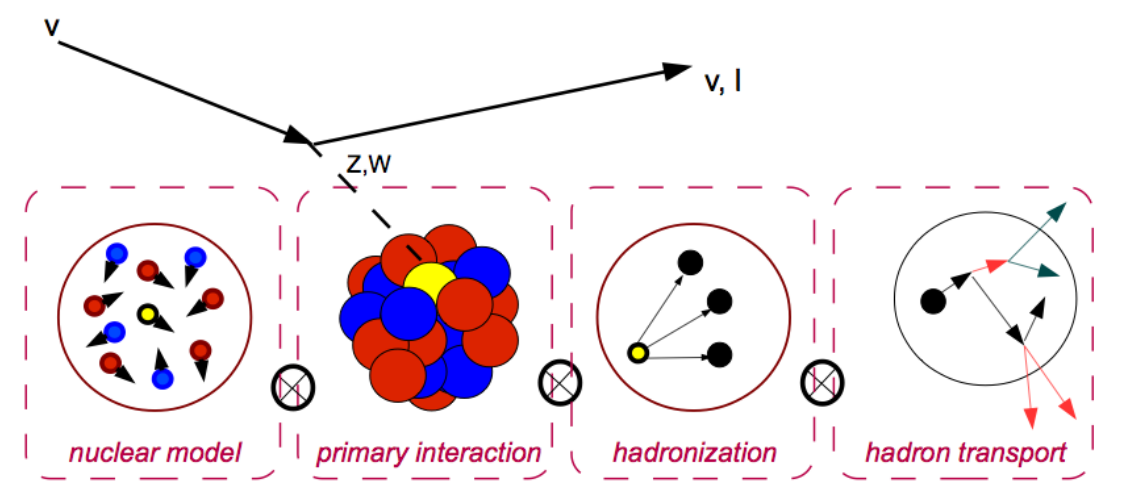
\includegraphics[width=.9\textwidth]{figures/x-secs/genie_models.png}
	\caption[Neutrino-Nucleus Scattering in \acrshort{genie}]{Neutrino-Nucleus Scattering in \acrshort{genie}: The full cross-section model to describe neutrino-nucleus interactions is split into nuclear, primary interaction, hadronisation and hadron transport models. Figure by C. Andeopoulos.}
	\label{fig:genie_models}
\end{figure}
%
In the following, mechanisms affecting the neutrino-nucleus cross-section predictions and related uncertainties are split into nuclear effects (\Cref{sec:nuclear_effects}) and neutrino-nucleus interaction processes ((\Cref{sec:nuclear_effects})).

\subsection{Nuclear Effects} \label{sec:nuclear_effects}
Nuclear effects are processes that result due to the aggregation of nucleons into nuclei. As there are more possibilities for the neutrino to interact with the nucleus' constituents and intermediate-state particles to undergo \acrshort{fsi}s inside the nuclear medium, the impact of nuclear effects in neutrino scattering becomes more relevant the heavier the nuclear target. Especially for future experiments with relatively heavy nuclear targets such as \acrshort{dune}, the knowledge of nuclear effects is essential to reduce uncertainties in cross-section estimations and in the neutrino energy reconstruction as nuclear effects distort outgoing particle kinematics. As shown schematically in \Cref{fig:nuclear_effects}, nuclear effects can be categorised into initial-state effects, nucleon correlation effects and \acrshort{fsi}s. Nuclear effects are important model element with respective associated uncertainties to be considered in the modelling of the neutrino-nucleus interaction process.
%
    \begin{figure}[bth]
	\centering \includegraphics[width=\textwidth]%{figures/x-secs/ise_fsis.png}
    %{figures/x-secs/nuclear_effects.pdf}
    {figures/x-secs/nuclear_effects_2.pdf}
	\caption[nucleareffects]{Nuclear Effects that complicate the description of neutrino-nucleus scattering. These can be categorised into initial state effects (left) such as Fermi motion, nucleon-binding processes (middle) for example via virtual pion exchange and final-state interactions (right) such as pion production or charge exchange within the nuclear medium in an intranuclear cascade model approach. The incoming muon neutrino $\nu_\mu$ represented by the black arrow followed by the dashed black line interacts via a charged-current quasi-elastic interaction with a neutron in an argon nucleus. A default fraction of pn-pairs inside the nuclear medium (left) prior to the neutrino interaction determines the frequency of neutrinos scattering off bound states of two nucleons. These give rise to different proton multiplicites (middle).
	The outgoing muon (indigo line) and proton (light blue line) traverse the nuclear medium. The proton can undergo various types of hadronic FSIs such as (in)elastic scattering, pion production, hadron absorption and charge exchange. Pions in this figure are shown in dark green ($\pi^+$), regular green ($\pi^-$), and light green ($\pi^0$). Figures taken or adapted from \cite{bathe-peters:2020, Bathe-Peters:2022kkj}.}
	\label{fig:nuclear_effects}
    \end{figure}
%
\paragraph{Initial-State Effects}
\acrlong{ise}s (\acrshort{ise}s) refer to any nuclear configuration prior to the neutrino interaction. Examples of \acrlong{ise}s (\acrshort{ise}s) are the nuclear binding energy resulting from the mass difference of the sum of all nucleons within the nucleus, the initial-state nucleon momentum distribution referred to as \acrfull{fm}, and Pauli-Blocking, in which two nucleons (being fermions) cannot simultaneously occupy the same quantum state, as well as multi-nucleon correlation effects (illustrated on the left in \Cref{fig:nuclear_effects}).

\paragraph{Multi-Nucleon Correlation Effects}
%
In 1955, Hideki Yukawa proposed a field between the neutron and proton that was later determined to be a virtual pion mediating color-charge exchange between two nucleons \cite{10.1143/PTPS.1.1}, which builds the conceptual framework for Long-Range nucleon-nucleon Correlations (\acrshort{lrc}s). More generally, a $n$-body current arising from $n$ nucleons bound by the exchange of virtual mesons is called \acrfull{mec} (schematically visualised on the left in \Cref{fig:nuclear_effects}). \acrshort{lrc}s mediated by $\pi$-, $\rho$- or $\omega$-mesons \cite{vancuyck} can redistribute energy transfers over all nuclear constituents over the whole size of the nucleus and lead to collective excitations such as resonances. In order to account for these mutual interactions of nucleons and to describe the structure of collective nuclear excitations, a generalisation of the Hartree-Fock mean-field approach know as \acrfull{rpa} \cite{Martini:2009uj,PhysRevC.81.045502} is implemented in modern neutrino event simulation tools. Nucleonic bound states can also form via so-called \acrlong{src}s (\acrshort{src}s) due to the interaction of quarks inside different nucleons, which account for $20\%-25\%$ of intranuclear nucleonic bound states \cite{RevModPhys.89.045002}. Short- and long-range correlations give rise to a nuclear potential $V(r)$ as shown in \Cref{fig:nucpot}.  \cite{vancuyck}
%
\begin{figure}[htb!]
	\centering
%	\includegraphics[width=.8\textwidth]{Images/nucpot.png}
	\includegraphics[width=.7\textwidth]{figures/x-secs/Nuclear_potential.pdf}
%	\includegraphics[width=.8\textwidth]{Images/Nuclear_potential4.pdf}
	\caption[Nucleon-Nucleon Correlation Potential]{Nucleon-Nucleon Correlation Potential $ V(r_{12})$ in dependence of the inter-nucleon distance $r_{12}$ given in units of the pion Compton wavelength $\kappa^{-1}\backsimeq 1.4$ fm: The $1\pi$-exchange potential determines the classical region (I). The $2\pi$-exchange potential determines the dynamical region (II) and \acrlong{src}s (\acrshort{src}s) dominate the phenomenological region (III). Figure adapted from \cite{10.1143/PTPS.3.1, Weise:2007pf}.}
	\label{fig:nucpot}
\end{figure}
%
Internucleon correlations may lead to a neutrino scattering off a bound state of two or more nucleons. Nucleon bonding by meson exchange in the nuclear medium allow the neutrino to interact with pairs of nucleons via \acrshort{mec}s. These multiple-body interactions can give rise to multi-nucleon excitations such as \acrshort{2p2h} or, generally more \acrshort{npnh} ($n>2$) excited states. Since these one, two or $n$ intermediate-state nucleons are then subject to further intranuclear rescattering processes, \acrshort{fsi}s after \acrshort{2p2h} excitation can result in final states experimentally indistinguishable from \acrshort{1p1h} processes.

\paragraph{\acrlong{fsi}s}
Once intermediate-state particles leave the neutrino-interaction vertex, they may experience intranuclear interactions with further nuclear constituents before exiting the nucleus as measurable final-state particles. Various \acrshort{fsi}s are illustrated on the right in \Cref{fig:nuclear_effects}. In a cascade model approach, the kinematics of intermediate-state particles can change, for example, in magnitude of momentum and direction by elastic and inelastic scattering, charge exchange, pion production, pion and hadron absorption. \acrshort{fsi}s become more difficult to seperate with increasing neutrino energy, because multiple \acrshort{fsi}s may result in the same final-state particles despite different neutrino-interaction processes.

\subsection{Neutrino-Nucleus Scattering} \label{sec:nu-nuc_scattering}
Neutrino-nucleus interactions are energy-dependent processes in which the neutrino interacts with a constituent of the nucleus or the nucleus itself. 
Different neutrino interaction processes scale with the energy of the incident neutrino and are associated with partial differential cross sections as shown in \Cref{fig:cc_inclusive_xsec_by_E}.
%
\begin{figure}[hbt]
	\centering
    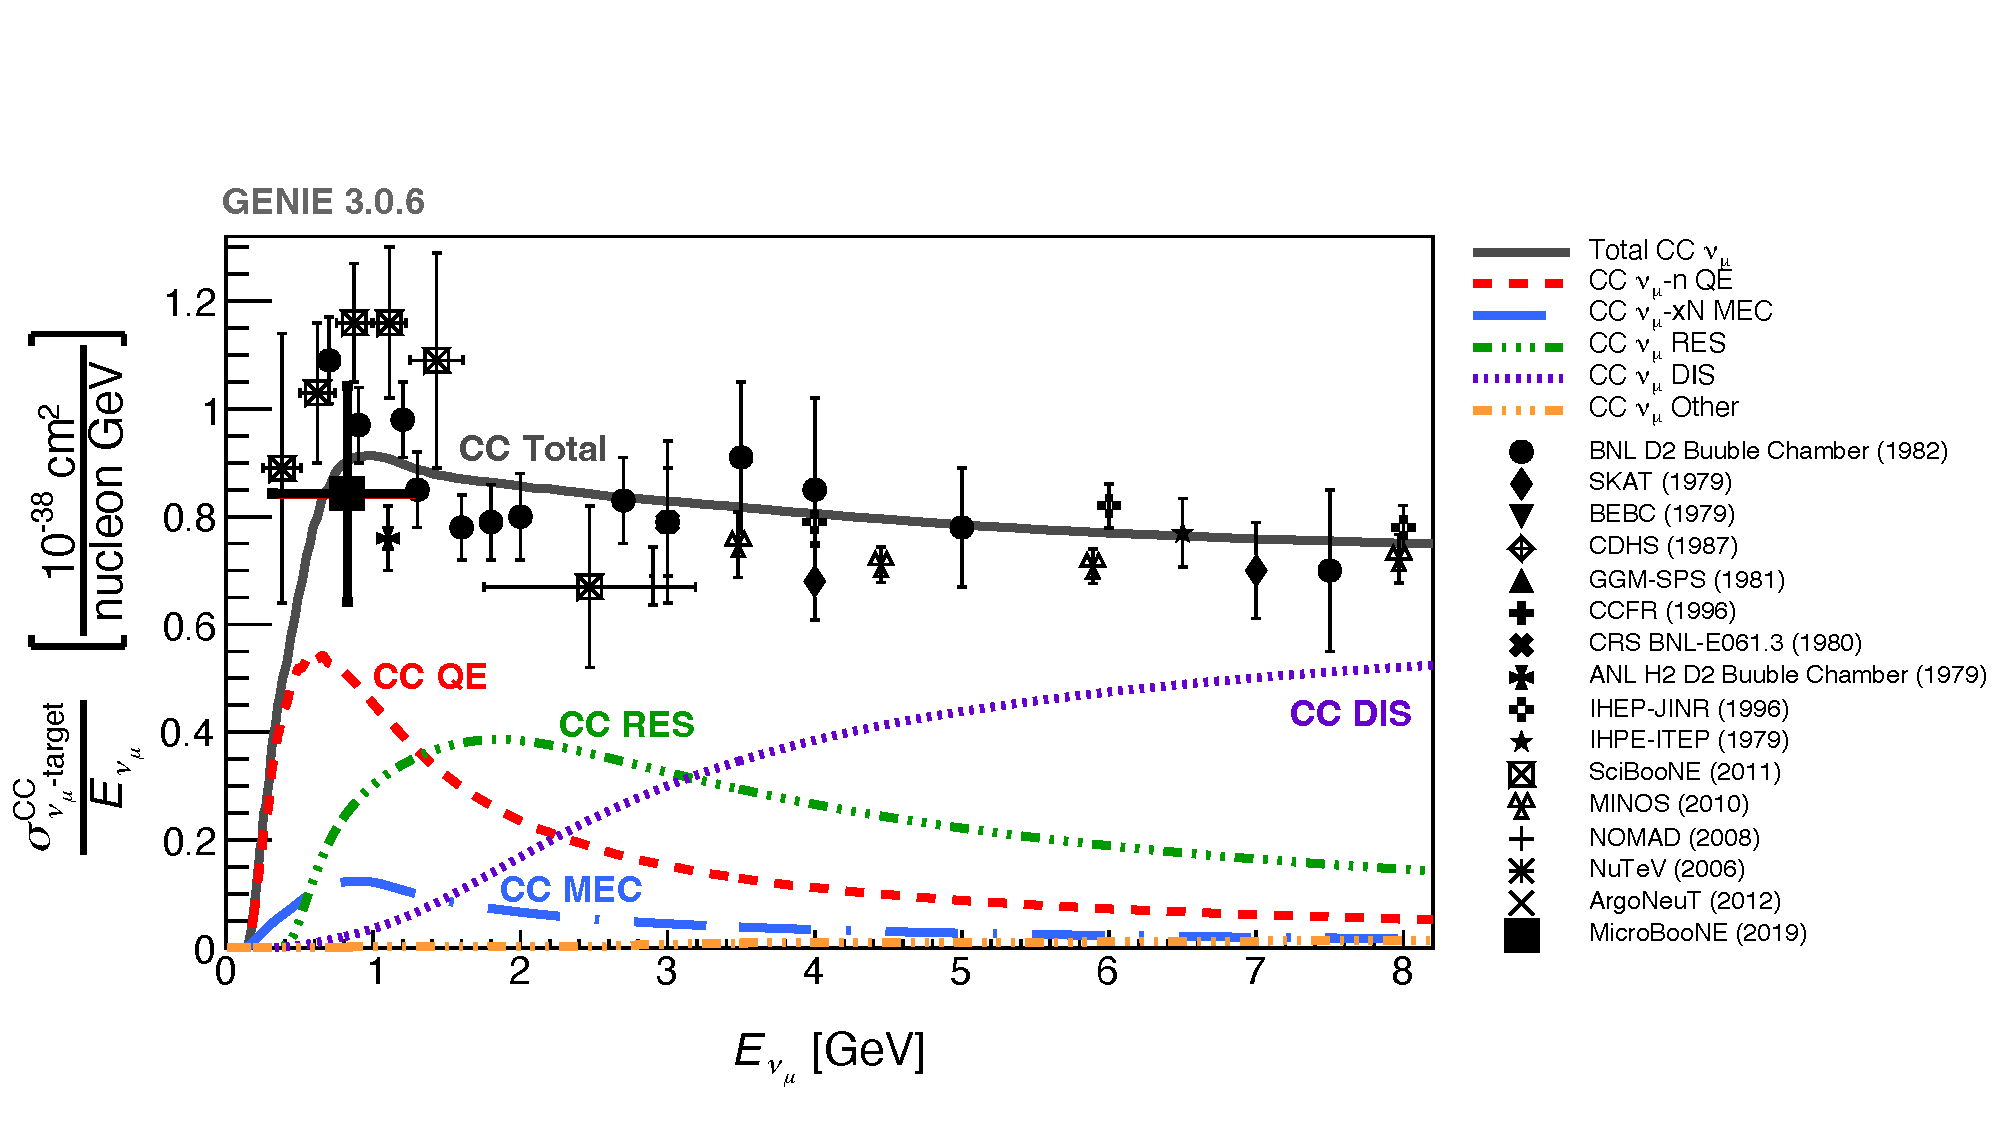
\includegraphics[width=\textwidth]{figures/x-secs/xsec_Ev_numu_split_uBooNE_black.pdf}
%	\begin{subfigure}[b]{\textwidth}
%	\includegraphics[width=\textwidth]{figures/xsec_Ev_log_legend.pdf}
%	    \includegraphics[width=\textwidth]{figures/xsec_Ev_numu_log_legend.pdf}
%	    \vspace{-6.mm}
%	    \caption{}
%	    \label{inclusive_xsec}
%	\end{subfigure}
%	    \vskip\baselineskip \vspace{-5.mm}
%	\begin{subfigure}[b]{\textwidth}
	    %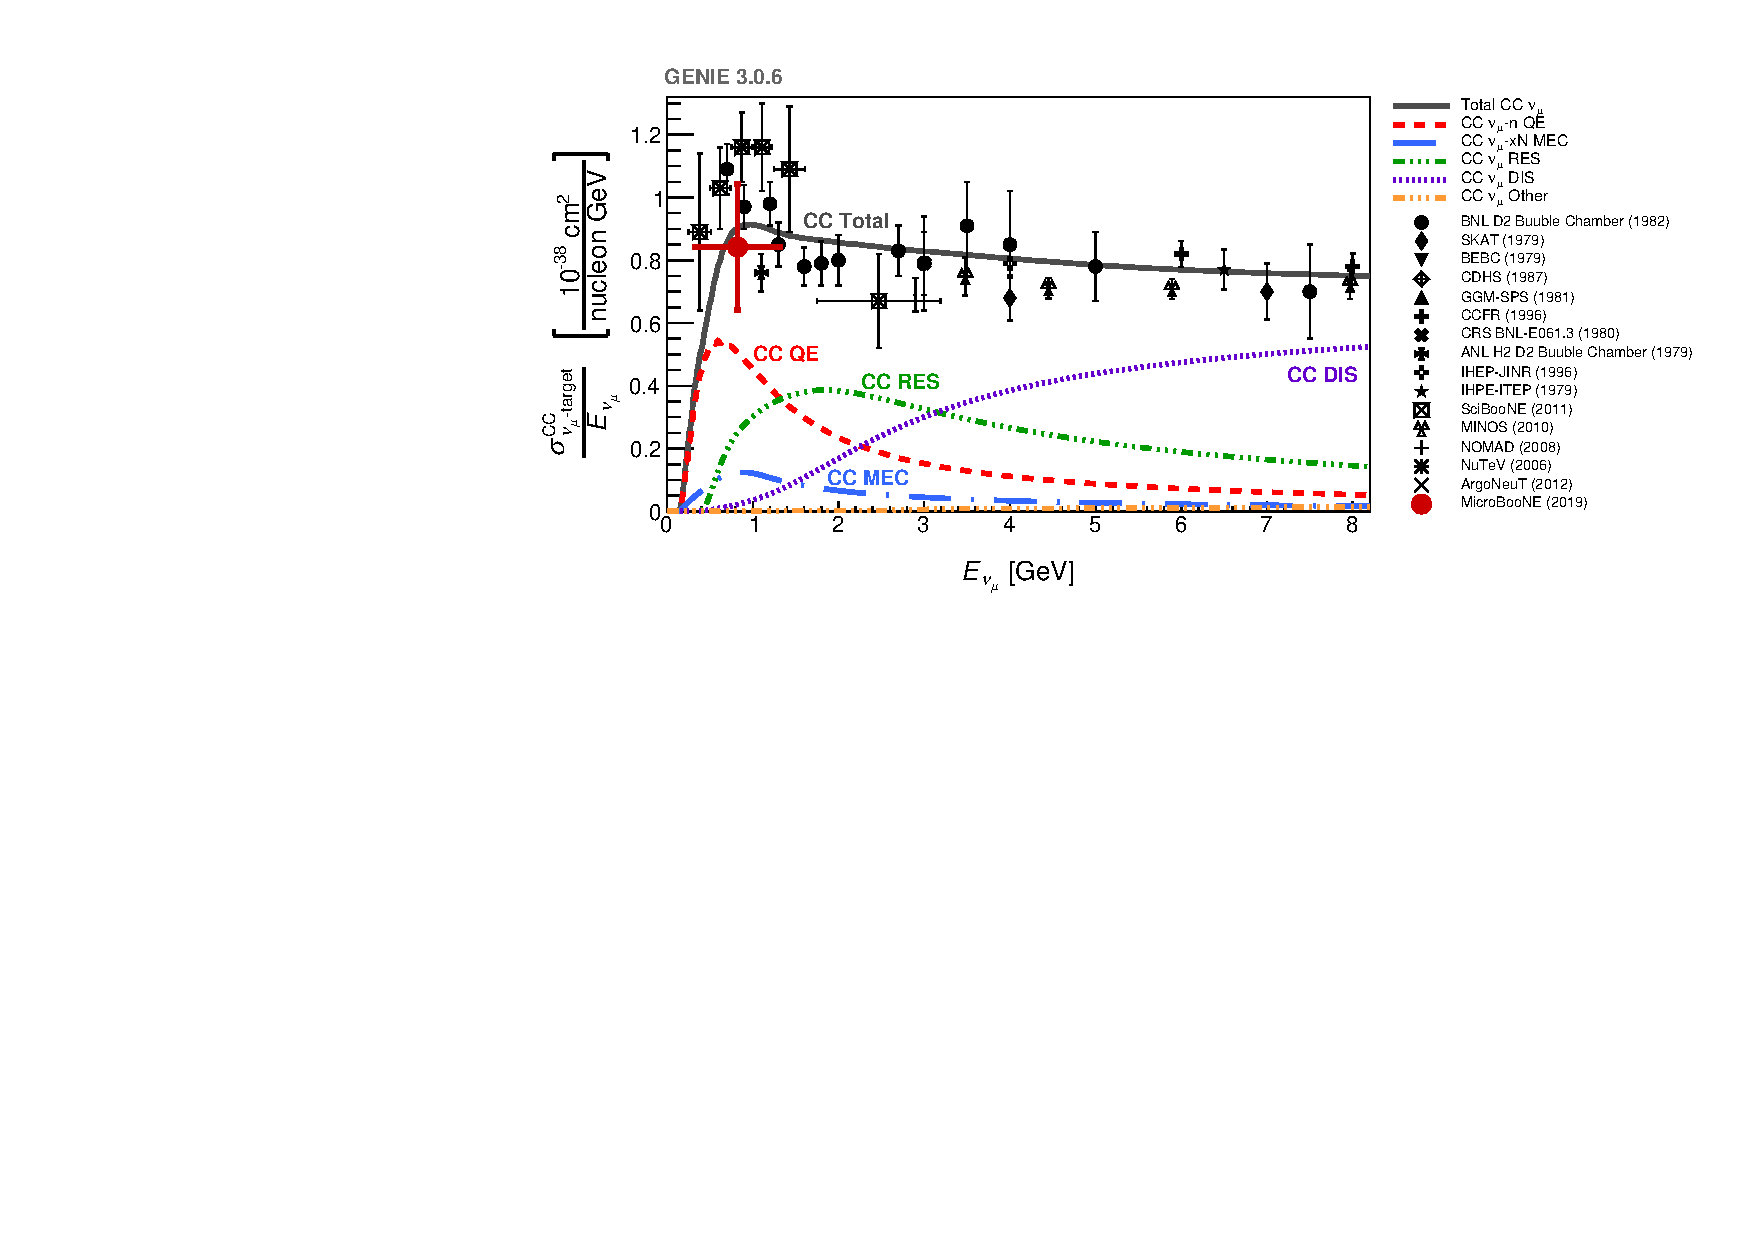
\includegraphics[width=\textwidth]{figures/x-secs/xsec_Ev_numu_split.pdf}
%	    \vspace{-6.mm}
%	    \caption{}
%	    \label{inclusive_xsec_split}
%	\end{subfigure}
\vspace{-3mm}
	\caption[Inclusive Charged-Current Cross Section]{Total inclusive muon neutrino per-nucleon charged-current cross section divided by and as a function of the neutrino energy $E_{\nu_\mu}$ (solid black). %The neutrino energy scales for each contributing interaction process.
% The \acrshort{cc}\acrshort{qe} (dashed red) process is dominant for neutrino energies below $1.5$GeV. \acrshort{cc}\acrshort{mec} is shown in dashed-dotted blue. %\subref{inclusive_xsec} The \acrshort{res} (light and dark green dashed-three-dotted line) and \acrshort{dis} (light and dark purple dotted line) cross sections include interactions on neutrons and protons that are summed in \subref{inclusive_xsec_split}.
%    Further contributing processes are coherent scattering (yellow), neutrino-electron scattering (light brown) and neutrino interactions with sea-charm quarks in \acrshort{qe} and \acrshort{dis} channels (dark brown). %\subref{inclusive_xsec_split} Zoom of \subref{inclusive_xsec} for a neutrino energy range $[0,8.3] \ \text{GeV}$. Analogous plots for $\bar{\nu}_\mu$ can be found in \Cref{xsec_Ev_numubar_log_legend} and \Cref{xsec_Ev_numubar_legend} in appendix \ref{appendix_a}, respectively. 
    Data was kindly provided by G. Zeller \cite{Formaggio:2013kya}. The MicroBooNE data point is taken from \cite{DelTutto:2019cpu}. Figure was taken from \cite{bathe-peters:2020}.}.
	\label{fig:cc_inclusive_xsec_by_E}
\end{figure}
%
\iffalse
%
    \begin{figure}[hbt]
    \centering
	\includegraphics[width=0.45\textwidth]%{figures/x-secs/2p2h_nu_Ar.png}
    {figures/x-secs/CCMEC_nu_Ar.pdf}
	\caption[Illustration of the \acrshort{2p2h} Scattering Process]{Illustration of the \acrlong{cc} $2\text{p}$-$2\text{h}$ scattering process: $\nu_\mu + 1\text{n}1\text{p} \rightarrow \mu^- + 2\text{p}$. In the absence of \acrshort{fsi}s, $2\text{p}$-$2\text{h}$ processes are all neutrino-nucleus interactions with two nucleons and no other hadrons. Here, a pion-in-flight \acrshort{mec} gives rise to a neutrino $2\text{p}$-$2\text{h}$ interaction. The incoming muon neutrino $\nu_\mu$ (black arrow) interacts with two nucleons ($2\text{p}$, here one proton shown in light blue and one neutron shown in grey) bound by a virtual meson (here $\pi$-meson shown in green), that are kicked out of the nucleus, so that the remnant nucleus is left with two holes $2\text{h}$ in the final state. Hereby, the $\text{W}^-$ boson mediates an electroweak \acrshort{cc} quark flavor change, so that a muon (indigo arrow) is produced and the inital-state neutron becomes a final-state proton.}
	\label{fig:mec_schematic}
\end{figure}
%
\fi
While low-energy neutrinos may coherently scatter off the whole nucleus, neutrinos with higher incident energy may resolve the nucleus as a bound state of nucleons, single nucleons or quarks inside the nucleons \cite{Bathe-Peters:2022kkj}. As shown in \Cref{fig:cc_inclusive_xsec_by_E}, different interaction processes are dominant at different energies \cite{bathe-peters:2020}. With increasing neutrino energy, the relative contributions to the total inclusive neutrino-interaction cross section shift from \acrshort{cc}\acrshort{qe} scattering dominance at low energies, through an intermediate energy range where \acrshort{cc} \acrshort{2p2h} and \acrshort{cc}\acrshort{res} interactions are significant, to ultimately \acrshort{cc}\acrshort{dis} processes at higher energies.

In \acrshort{cc}\acrshort{qe} ($\accentset{\brobor\vspace{-.5mm}}{\nu}_\ell + \text{N} \rightarrow \ell{\hspace{0.1ex}'}^{\hspace{0.1ex} \accentset{(+)\vspace{-.8mm}}{-}} + \text{N}'$) interactions without subsequent \acrshort{fsi}s (upper right in \Cref{fig:nu_int_scale}), the incoming neutrino $\nu_\mu$ (black arrow in \Cref{fig:nu_int_scale}) interacts with a single neutron n (gray) via a weak \acrshort{cc} interaction mediated by a W-boson, producing a muon (indigo arrow) and proton (light blue arrow).
In \acrshort{cc} \acrshort{2p2h} ($\accentset{\brobor\vspace{-.5mm}}{\nu}_\ell + 2\text{N} \rightarrow \ell{\hspace{0.1ex}'}^{\hspace{0.1ex} \accentset{(+)\vspace{-.8mm}}{-}} + 2\text{N}'$) scattering, the interaction instead involves a correlated pair of nucleons (gray and light blue in \Cref{fig:nu_int_scale}) in the initial state, as further described in \Cref{sec:2p2h_scattering}.
In order for \acrshort{cc}\acrshort{res} ($\accentset{\brobor\vspace{-.5mm}}{\nu}_\ell + \text{N} \rightarrow \ell{\hspace{0.1ex}'}^{\hspace{0.1ex} \accentset{(+)\vspace{-.8mm}}{-}} + \text{N}^* \rightarrow \ell{\hspace{0.1ex}'}^{\hspace{0.1ex} \accentset{(+)\vspace{-.8mm}}{-}} + \text{N}' + X\pi'$) to occur, the neutrino-nucleon scatter must transfer sufficient energy such that the invariant mass of the hadronic system $W$ lies in the resonance region to excite the nucleon to a baryon resonance state $\text{N}^* \equiv \Delta (1232)$ (purple in \Cref{fig:nu_int_scale}). This resonance subsequently decays into a nucleon $\text{N}'$ (light blue) and one or more pions $\pi'$ (green) in the final state.
At sufficiently high energies, \acrshort{cc}\acrshort{dis} ($\accentset{\brobor\vspace{-.5mm}}{\nu}_\ell + \text{q} \rightarrow \ell{\hspace{0.1ex}'}^{\hspace{0.1ex} \accentset{(+)\vspace{-.8mm}}{-}} + \text{X}'$) occurs whne the neutrino scatters off a quark inside a nucleon. This process can result in the production of hadronic jets and the breakup of the nucleus.

As future \acrshort{lbl} neutrino oscillation experiments exploit higher-energetic neutrino beams, the contribution of \acrshort{2p2h} processes and their modeling with associated uncertainties becomes increasingly important. 
Since \acrshort{dune} will operate at neutrino energies in the range of $0.5$-$3.5$ GeV \cite{DUNE:2020ypp}, where \acrshort{2p2h} interactions are significant, they constitute a key component of the neutrino interaction model. 
\Cref{fig:nu_int_scale} shows the unoscillated near detector flux predictions of the neutrino \acrlong{lbl} oscillation experiments \acrshort{dune}, \acrshort{nova} and \acrshort{t2k} overlaid with the total and partial neutrino cross-section predictions for various neutrino-interaction channels that are schematically shown in \Cref{fig:nu_exp_fluxes}.
%
    \begin{figure}[htb]
	\centering
	\includegraphics[width=\textwidth]%{Images/nu_nuc_xsecs.pdf}
    {figures/x-secs/nu-nuc_int.png}
	\caption[Illustrations of Neutrino-Nucleus Interactions]{Schematic illustration of the main neutrino-nucleus interaction modes: \acrfull{qe} (upper left, green), \acrfull{2p2h} (upper right, yellow), \acrfull{res} (lower left, orange), \acrfull{dis} (lower right, red). The frame colours correspond to the respective partial cross-section shown in \Cref{fig:nu_exp_fluxes}, which demonstrates the different energy-scaling of these neutrino-interaction processes. Figures taken or adapted from \cite{bathe-peters:2020}.}
	\label{fig:nu_int_scale}
    \end{figure}
%
%
    \begin{figure}[hbt]
	\centering
	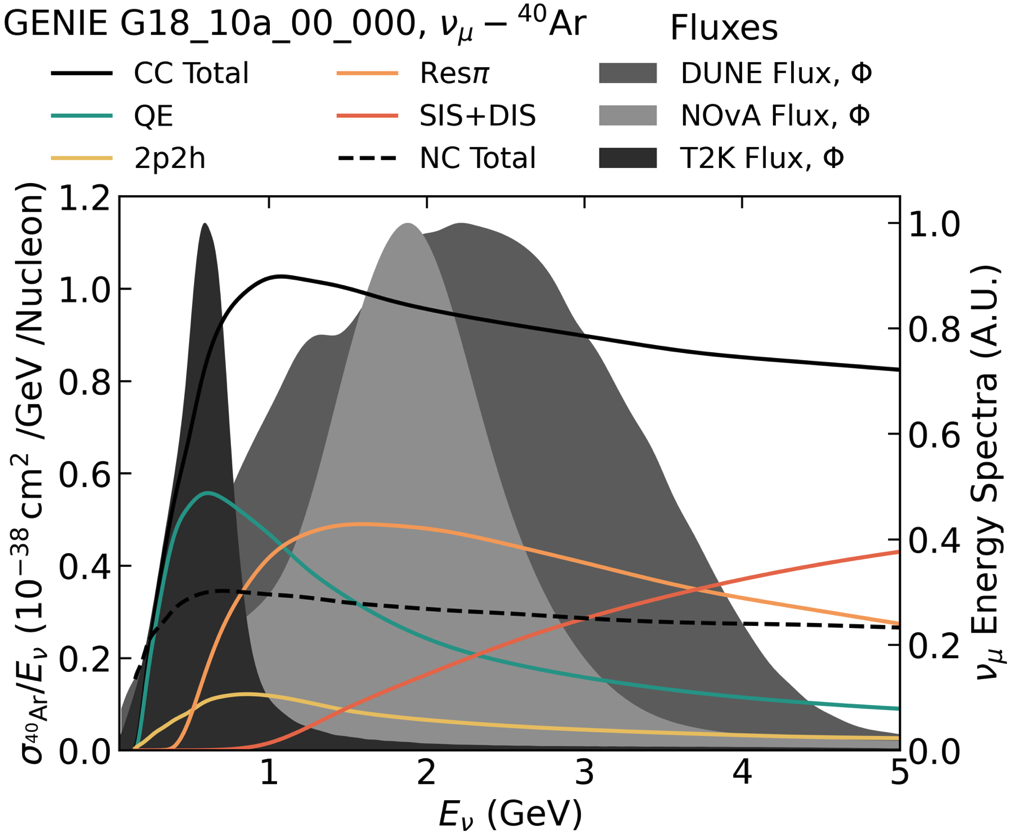
\includegraphics[width=.8\textwidth]{figures/x-secs/exp_fluxes.png}
	\caption[DUNE, T2K and No$\nu$a Fluxes overlaid with Cross Sections]{Unoscillated DUNE, No$\nu$a and T2K flux predictions overlaid with neutrino-argon cross sections as a function of the neutrino energy. Plot from L. Pickering.}
	\label{fig:nu_exp_fluxes}
    \end{figure}
%
Although subdominant, \acrshort{2p2h} interactions constitute a significant contribution in the energy range relevant for future experiments (as it can be seen in \Cref{fig:nu_int_scale}), making their accurate modelling and uncertainty development essential. For a more detailed overview of nuclear effects and neutrino-nucleus interaction processes, see for example \cite{bathe-peters:2020}.

\section{Neutrino 2-Particle-2-Hole Scattering} \label{sec:2p2h_scattering}
%
As it was described in \Cref{sec:nu-nuc_scattering}, the formation of nucleons into bound pairs inside the nucleus enables the neutrino to scatter off bound states of two (or more) nucleons in a so-called \acrshort{2p2h} neutrino-nucleus scattering event giving raise to a lepton and two particles in the final state (see \Cref{mec_schematic}). In the absence of \acrshort{fsi}s, the \acrshort{2p2h} interaction is a neutrino interaction on two particles leaving two holes inside the nucleus \cite{Gran:2013kda}, hence the name \acrlong{2p2h} interactions. Various processes for the \acrshort{cc} or \acrshort{nc} two-body interaction between a gauge boson $\text{X}$ with a virtual pion $\pi$ or a nucleon $\text{N}$ as a result of \acrshort{mec}s giving rise to neutrino $1\text{p}$-$1\text{h}$ or $2\text{p}$-$2\text{h}$ processes. In contact or seagull currents, the boson couples with the \acrshort{mec} at the $\pi-\text{NN}$ vertex. Pion-in-flight currents refer to a boson $\text{X}$ coupling with the virtual pion $\pi$. In isobar ($\Delta$) currents, the boson $\text{X}$ interacts with the nucleon and excites it to a virtual delta baryon $\Delta$ following its deexcitation under the exchange of a $\pi$-meson with the other nucleon. Finally, correlation currents involve a nucleon $\text{N}$ that propagates between the $\pi$-\acrshort{mec} and the interaction vertex with boson $\text{X}$ \cite{vancuyck}.
\Cref{fig:nu_int_scale} provides an illustration of the \acrlong{cc} $2\text{p}$-$2\text{h}$ scattering process: $\nu_\mu + 1\text{n}1\text{p} \rightarrow \mu^- + 2\text{p}$. In the absence of \acrshort{fsi}s, $2\text{p}$-$2\text{h}$ processes are all neutrino-nucleus interactions with two nucleons and no other hadrons. Here, a pion-in-flight \acrshort{mec} gives rise to a neutrino $2\text{p}$-$2\text{h}$ interaction. The incoming muon neutrino $\nu_\mu$ (black arrow) interacts with two nucleons ($2\text{p}$, here one proton shown in light blue and one neutron shown in grey) bound by a virtual meson (here $\pi$-meson shown in green), that are kicked out of the nucleus, so that the remnant nucleus is left with two holes $2\text{h}$ in the final state. Hereby, the $\text{W}^-$ boson mediates an electroweak \acrshort{cc} quark flavor change, so that a muon (indigo arrow) is produced and the inital-state neutron becomes a final-state proton.
The importance of these multi-nucleon channels was recognised in early works such as \cite{Martini:2009uj}, and they are now understood to constitute a significant source of uncertainties in neutrino–nucleus cross-section modelling \cite{Niewczas:2019fro}.
Clarifying the degree to which it can be distinguished from look-alike processes \cite{PhysRevC.98.045502} in argon and to have the ability to correctly account for uncertainties from differences between models is therefore of substantial interest. For example, as \acrshort{fsi}s can obscure the topology of the primary neutrino interaction, they may lead to the absorption of one of the two intermediate-state nucleons produced at the \acrshort{2p2h} neutrino interaction vertex. Hence, \acrshort{fsi}s make it experimentally very challenging to distinguish \acrshort{cc}\acrshort{qe}-like \acrshort{2p2h} from \acrshort{cc}\acrshort{qe} interactions with the same final-state topology \cite{Furmanski:2016wqo,Niewczas:2019fro}. The historical insights that lead to realise the importance of including \acrshort{2p2h} interactions in the cross-section model is demonstrated in \Cref{fig:MB_puzzle}. In summary, it is important to model \acrshort{2p2h} interactions in order to reproduce inclusive cross-section data, as calculations including only \acrshort{qe} contributions tend to underpredict the cross section in the dip region (see left plot in \Cref{fig:MB_puzzle} \cite{Benhar:2006wy}). This discrepancy has been attributed to multi-nucleon (\acrshort{2p2h}) processes arising from \acrshort{mec}s, whose inclusion fills in the dip (left in \Cref{fig:MB_puzzle} \cite{Benhar:2006wy}) and improves agreement with data (right in \Cref{fig:MB_puzzle} \cite{PhysRevD.81.092005,PhysRevC.81.045502}).
%
\begin{figure}[b!]
		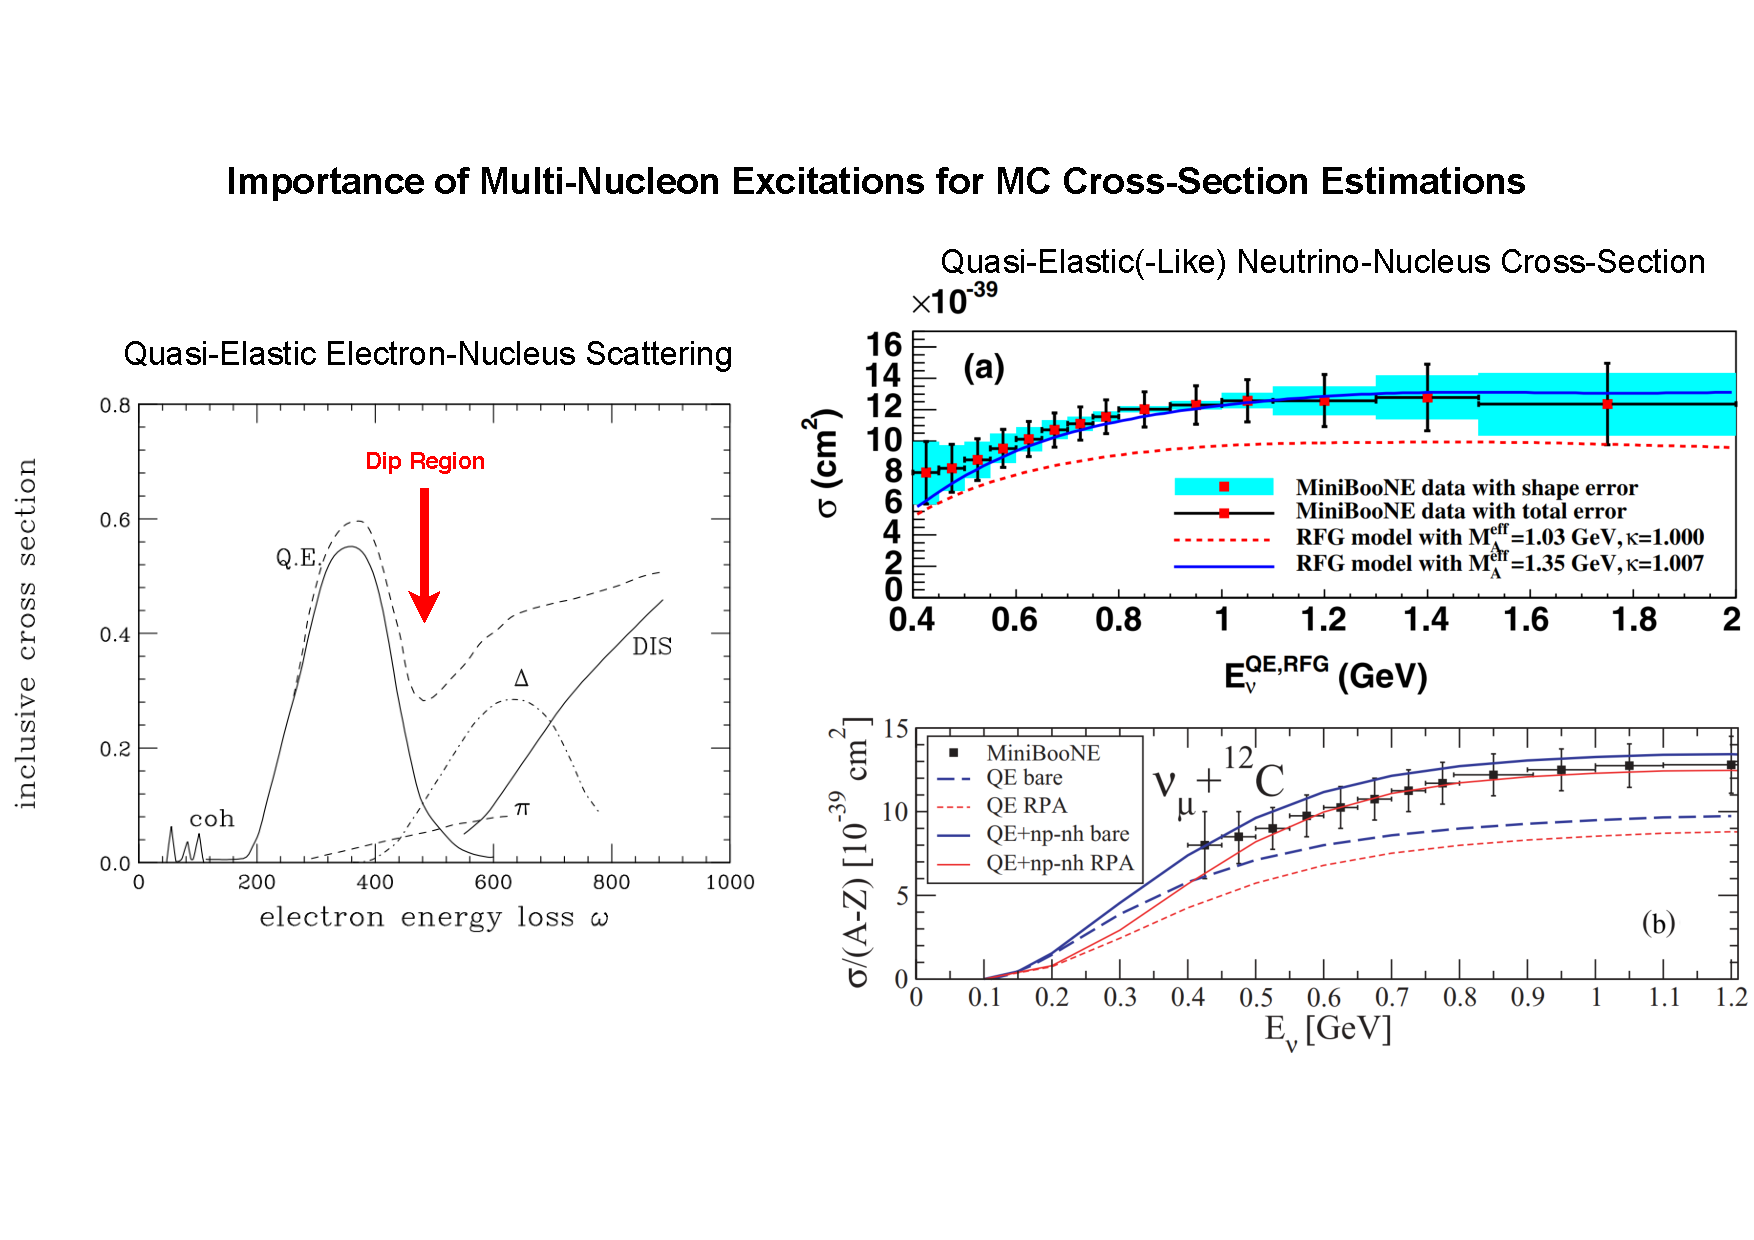
\includegraphics[width=\textwidth]{figures/x-secs/ccqe-like-measurements.pdf}
	\caption[Underestimation of Inclusive Cross-Sections]{Underestimation of Inclusive Cross-Sections. Left: Inclusive \acrshort{qe} electron-nucleus cross section as a function of the electron-energy loss $\omega$. Previously neglected \acrshort{npnh} contributions arising from \acrshort{mec}s provide for additional strength in the dip region (red arrow) between the \acrshort{qe} and \acrshort{res} peaks in electron-nucleus scattering data. Figure adapted from \cite{Benhar:2006wy}.
    %
    Right: Flux-unfolded MiniBooNE $\nu_\mu$ (\textit{pure}) \acrshort{cc}\acrshort{qe} cross section per neutron as a function of neutrino energy. Upper pannel: Measurement by the MiniBooNE collaboration showing the data excess of this \textit{pure} \acrshort{cc}\acrshort{qe} process on carbon with an extracted axial mass of $M_\text{A}^{\text{eff}} = 1.35 \pm \SI{0.17}{\GeV}$, significantly higher than the expected world-average value $M_\text{A} = \SI{1.03}{\GeV}$. Figure taken from \cite{PhysRevD.81.092005}.
    %
    Lower pannel: \acrshort{cc}\acrshort{qe}-\textit{like} cross section per neutron with and without multi-nucleon processes and \acrshort{rpa} effects included as a function of the neutrino energy. The inclusion of multi-nucleon excitations reconciles the discrepancy by accounting for the missing strength in the \acrshort{mc} prediction. Figure taken from \cite{PhysRevC.81.045502}.}
	\label{fig:MB_puzzle}
\end{figure}
%
A particular powerful set of observables that are especially sensitive to nuclear effects are the so-called \acrfull{tki} variables \cite{Lu:2018stk}, which are constructed from imbalance in the transverse kinematics of the final-state particles. Different regions of \acrshort{tki} phase-space exhibits enhanced sensitivity to specific nuclear effects, allowing discrimination between interaction mechanisms such as \acrshort{cc}\acrshort{qe}, \acrshort{2p2h}, and \acrshort{fsi} contributions \cite{Bathe-Peters:2022kkj}.

\subsection{\texorpdfstring{\acrlong{cc}}{TEXT} 2p-2h Models} \label{subsec:model_comparisons} 
%
The differences in the theoretical computations of the 2p-2h process in the Valencia, SuSAv2 and Martini-Ericson-Chanfray-Marteau (Martini et al) models are summarised in \cref{tab:2p2h_models}.
%
    \begin{figure}[hbt]
	\centering
	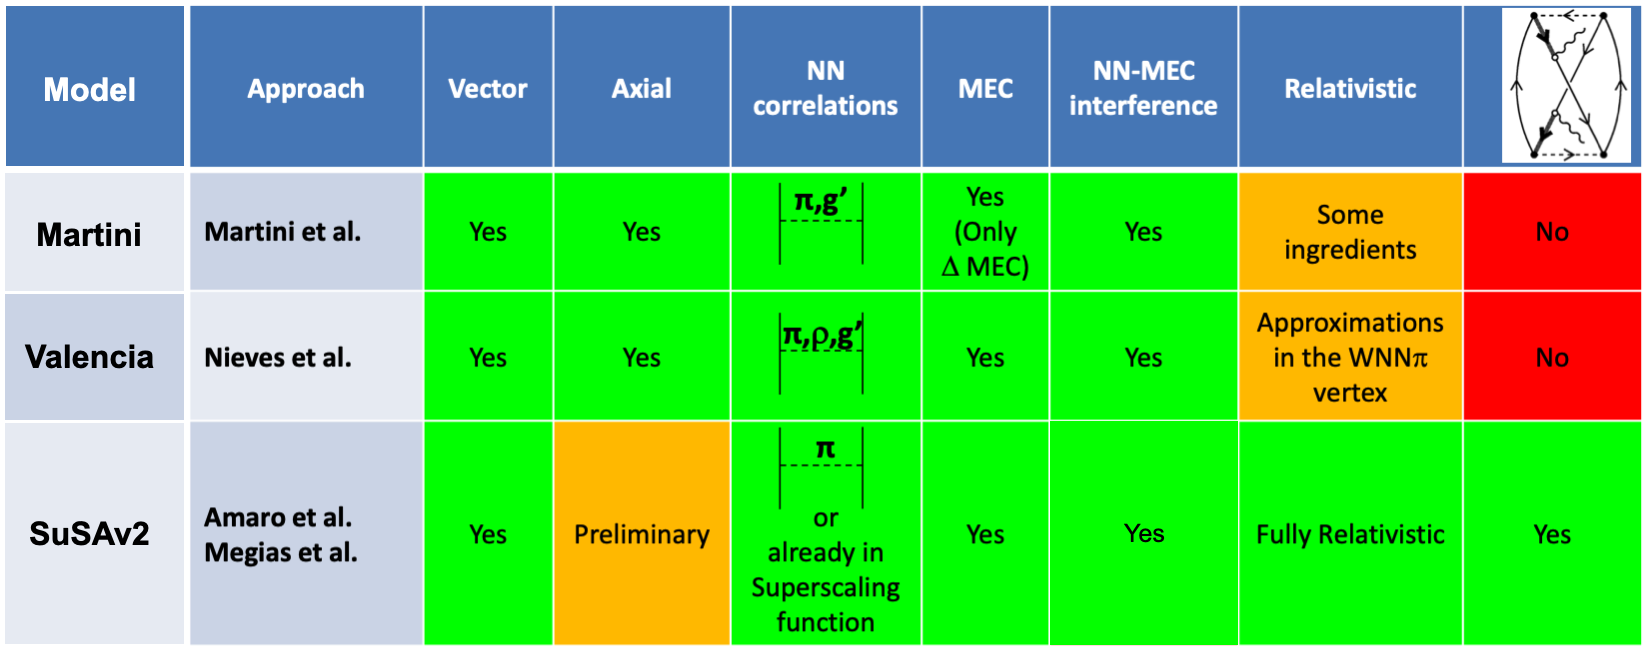
\includegraphics[width=\textwidth]{figures/x-secs/2p2h_models_table.png}
	\caption[2p2hmodels]{Charged-current 2p-2h model differences in the Martini, Valencia and the SuSAv2 models. Table adapted from \cite{martini2016}.}
	\label{tab:2p2h_models}
    \end{figure}
    \vspace{-4mm}
%
The primary distinctions between these models arise from the contributing Feynman diagrams and the treatment of interference effects of associated nuclear resonances.
In addition to the models listed in \cref{tab:2p2h_models}, an empirical \acrshort{mec}-based \acrshort{2p2h} model is implemented in the GENIE neutrino event generator.
The results presented in this chapter are obtained from simulations of muon-neutrino interactions on argon using the GENIE neutrino event generator with implemented \acrshort{cc} \acrshort{2p2h} Empirical, Valencia, SuSAv2 and Martini et al. models. The corresponding model set configurations are listed in \cref{tab:new_tunes}.
%
\begin{table}[htb]
	\caption[Elements of \acrshort{genie} Model Sets used in the Simulation of Muon-Neutrino Interactions on Argon]{Elements of \acrshort{genie} Model sets used in the simulation of muon-neutrino interactions on argon. The neutrino-nucleus interaction is described by a combination of nuclear ground-state model, \acrfull{qe}, \acrfull{2p2h} (\acrshort{mec}) \acrfull{res}, \acrfull{dis}, \acrfull{coh} processes and \acrfull{fsi}s.}\label{tab:new_tunes}
\resizebox{\textwidth}{!}{
	\begin{tabular}{|l||c|c|c|c|}
		\hline
		\diagbox{\textbf{Model}}{\textbf{Set}} & $\mathtt{G18\_10a\_00\_000}$ & $\mathtt{G18\_10s\_00\_000}$ &  $\mathtt{G18\_10e\_00\_000}$ & $\mathtt{G18\_10m\_00\_000}$ \\ \hline \hline
		Nuclear Model	& Local Fermi Gas & Local Fermi Gas & Local Fermi Gas & Local Fermi Gas \\ \hline
		\acrshort{qe} &  Nieves & Nieves & Nieves & Nieves \\ \hline
		\cellcolor{yellow!20}\acrshort{2p2h} (\acrshort{mec})	& \cellcolor{yellow!20}Nieves (Valencia) & \cellcolor{yellow!20}SuSAv2 & \cellcolor{yellow!20}Empirical & \cellcolor{yellow!20}Martini-Ericson-Chanfray-Marteau \\ \hline
		\acrshort{res}	& Berger-Sehgal & Berger-Sehgal & Berger-Sehgal & Berger-Sehgal \\ \hline
  		\acrshort{dis}	& Bodek-Yang & Bodek-Yang & Bodek-Yang & Bodek-Yang \\ \hline
		\acrshort{coh}	& Berger-Sehgal & Berger-Sehgal & Berger-Sehgal & Berger-Sehgal \\ \hline
		\acrshort{fsi}s	& INTRANUKE hA 2018 & INTRANUKE hA 2018 & INTRANUKE hA 2018 & INTRANUKE hA 2018 \\ \hline
	\end{tabular}
    } % end of resizebox
\end{table}
%
The aim of this study is to define systematic uncertainties that are sufficiently conservative to avoid biases in the extracted oscillation parameters arising from model mis-specification. Hereby, systematic parameters provide means to challenge and depart from the underlying physics assumptions of the nominal prediction, which for DUNE corresponds to the \acrshort{cc} 2p-2h SuSAv2 model. This is achieved by the method of event reweighting.

\section{2-Particle-2-Hole Systematic Uncertainty Parameters} \label{sec:2p-2h_unc}
%Briefly describe DUNE and why it is good for measuring 2p2h cross sections...
%
In order to theoretically predict and experimentally understand data associated with neutrino-nucleus cross sections, the \acrshort{genie} neutrino event generator performs simulations of neutrino interactions according to underlying theoretical models. A number of novel parameters have been implemented to allow new degrees of freedom in the uncertainty model. In the future, these parameters will be constrained by fitting them to experimental data, ultimately giving rise to a GENIE theory-driven uncertainty model \cite{PhysRevD.105.072001}. % The hoped outcome is a better simulation-data agreement with improved uncertainties based on the fit.
This will provide sufficient freedom in the \acrshort{dune} model to fit the eventual data without bias.

\subsection{Propagating Uncertainties} 
%
%Any nominal \acrfull{mc} prediction $P$ such as a physical parameter (e.g. axial mass) or a function of a kinematical parameter (e.g. a cross section as a function of energy) as a neutrino-generator input physics quantity cannot be easily expressed analytically or tabulated. 
Since it is too costly in terms of time and resources to (re)generate \acrshort{mc} simulations for every change in every parameter, evaluating uncertainties via reweighting is more feasible to vary parameters, e.g. in a fit to data. For each systematic uncertainty, a parameter $x_\text{P}$ is introduced to vary the nominal prediction. When applicable, this corresponds to a shift in a physical parameter $P$, while in other cases it modifies the kinematic distribution or interaction model directly through reweighting.







%
%Describe plots of chosen variables from plotting script... show GENIEReweight plots, explain them...; what can we get out of them?...
%Can area-normalise plots in geniev3plottingscript in worst case scenario
In order to interpret data, studies of accelerator neutrinos rely on detailed simulations of beam production, neutrino scattering, final-state particle transport and the detector response. Neutrino event generators such as \acrshort{genie} have models of neutrino cross sections implemented. %However, due to the lack of a comprehensive theoretical framework that can predict all observables for all interaction modes, the current approach for neutrino event generators is to adopt a factorisation scheme in which model components are joined together to fully simulate the scattering process. In that manner, the simulation of a typical neutrino-nucleus scattering event first involves the interaction mode and initial particle kinematics. Then, outgoing kinematics for the final-state particles are chosen according to the differential cross section appropriate for the sampled interaction mode. The event simulation finishes after considering intranuclear rescattering of the outgoing hadrons using a \acrshort{fsi} model. \cite{Bathe-Peters:2022kkj}
For the results shown in this report, I used \acrshort{genie} v$3.4.0$ with different model configurations. In all configurations, a \acrfull{lfg} model is used to describe the nuclear ground state prior to the neutrino interaction. % In the $\verb!G18_10a!$ model set, \acrshort{cc}\acrshort{qe} and \acrshort{2p2h} scattering are simulated using the $1$p$1$h and \acrshort{2p2h} Valencia model, respectively. Long-range nucleon-nucleon correlations are accounted for in this model via the \acrfull{rpa}. Resonance and coherent pion production are modeled by the Berger and Sehgal model \cite{Berger:2008xs}. The Bodek and Yang model \cite{Bodek:2002vp} is used for \acrshort{dis} and \acrshort{fsi}s are simulated using an intranuclear cascade model called $hA2018$ \cite{Dytman2021}. 
For this analysis, the most important difference when considering the results shown below is to consider the three different \acrshort{2p2h} models used to simulate \acrshort{2p2h} scattering. These are the Empirical, Valencia and SuSAv$2$ \acrshort{cc} \acrshort{2p2h} models, whereby the latter one is intended to be the default model for \acrshort{dune}. The goal is to develop reweighting parameters that will go from the SuSAv$2$ model to predictions from other models.
%While the $\verb!G18_01a!$ model set uses the GENIE Empirical \acrshort{cc} \acrshort{2p2h} model, the $\verb!G18_10a!$ model set employs the Valencia \acrshort{cc} \acrshort{2p2h} model. The remaining model configuations use the SuSAv$2$ \acrshort{cc} \acrshort{2p2h} model.

%\subsection{Comparison of Models}
%In the following three different sets of plots are shown. The first set of plots in \Cref{set1} shows effects of \acrshort{fsi}s on chosen variable distributions. 
%In the second set of plots in \Cref{set2}, the current \acrshort{cc} \acrshort{2p2h} models being implemented in the neutrino event generator GENIE are compared and differences that allow possible discrimination between the models are highlighted. 
%The systematic parameters described in \Cref{systematic_parameters} are evaluated in \Cref{set3}.



%
%3 models postFSI (according to equally likely data, phase space that is covered by reasonable models that we want to cover by uncertainties-> uncertainties)
Due to insufficient \acrshort{mc}-data agreement for the current \acrshort{cc} \acrshort{2p2h} models, one has to account for differences between these models in associated uncertainties. The set of plots in \Cref{set2_plots} provides a direct comparison and highlights possible discrimination between the available \acrshort{cc} \acrshort{2p2h} models at present in GENIE.
%
\begin{figure}[htb!]
	\begin{subfigure}[b]{.325\textwidth}
%        \includegraphics[width=\textwidth]{figures/1DComp_ErecAbsBias_14_ccmec.pdf}
        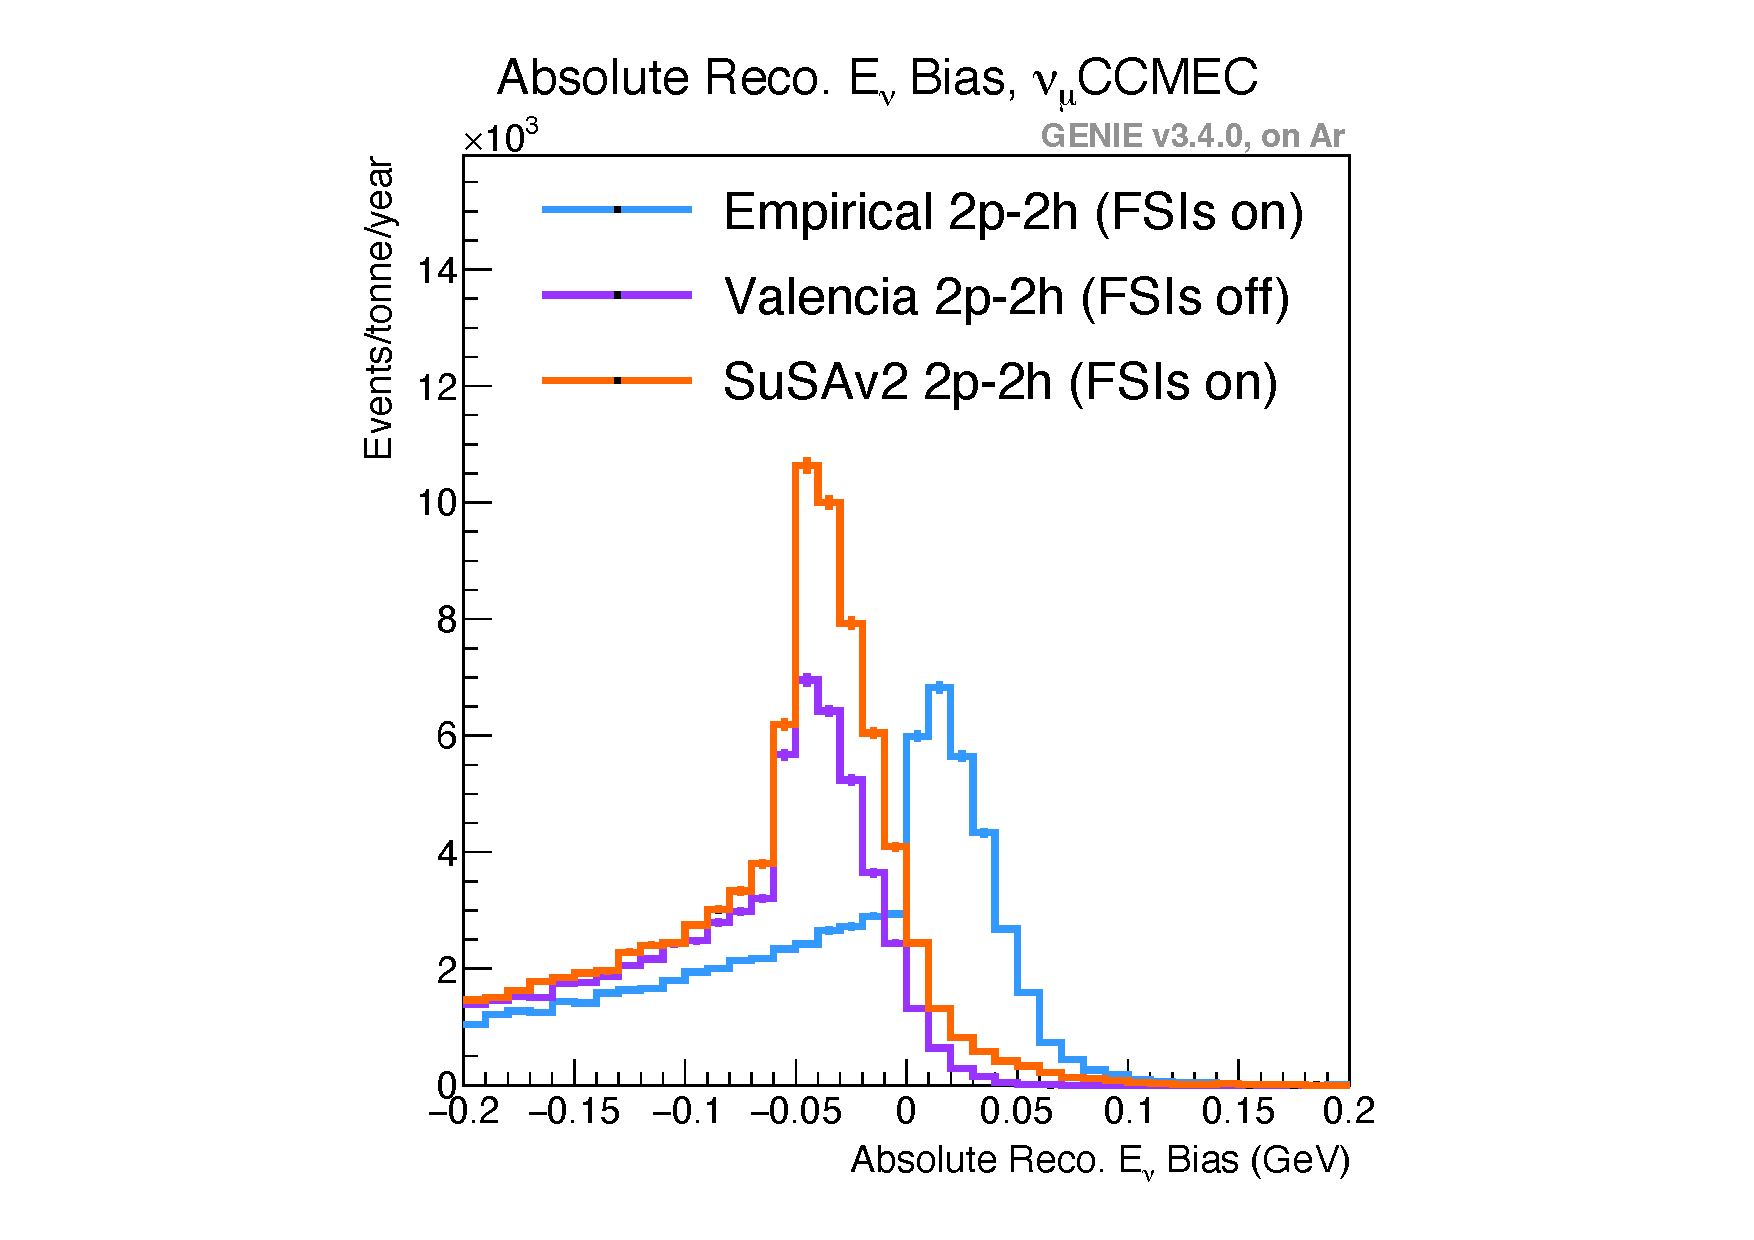
\includegraphics[width=\textwidth]{figures/postFSIs/1DComp_ErecAbsBias_14_ccmec_edited.pdf}
%        \vspace{-2.mm}
% \caption{}
	\label{set2_a}
    \end{subfigure}
	\begin{subfigure}[b]{.305\textwidth}
%        \includegraphics[width=\textwidth]{figures/1DComp_ErecRelBias_14_ccmec.pdf}
        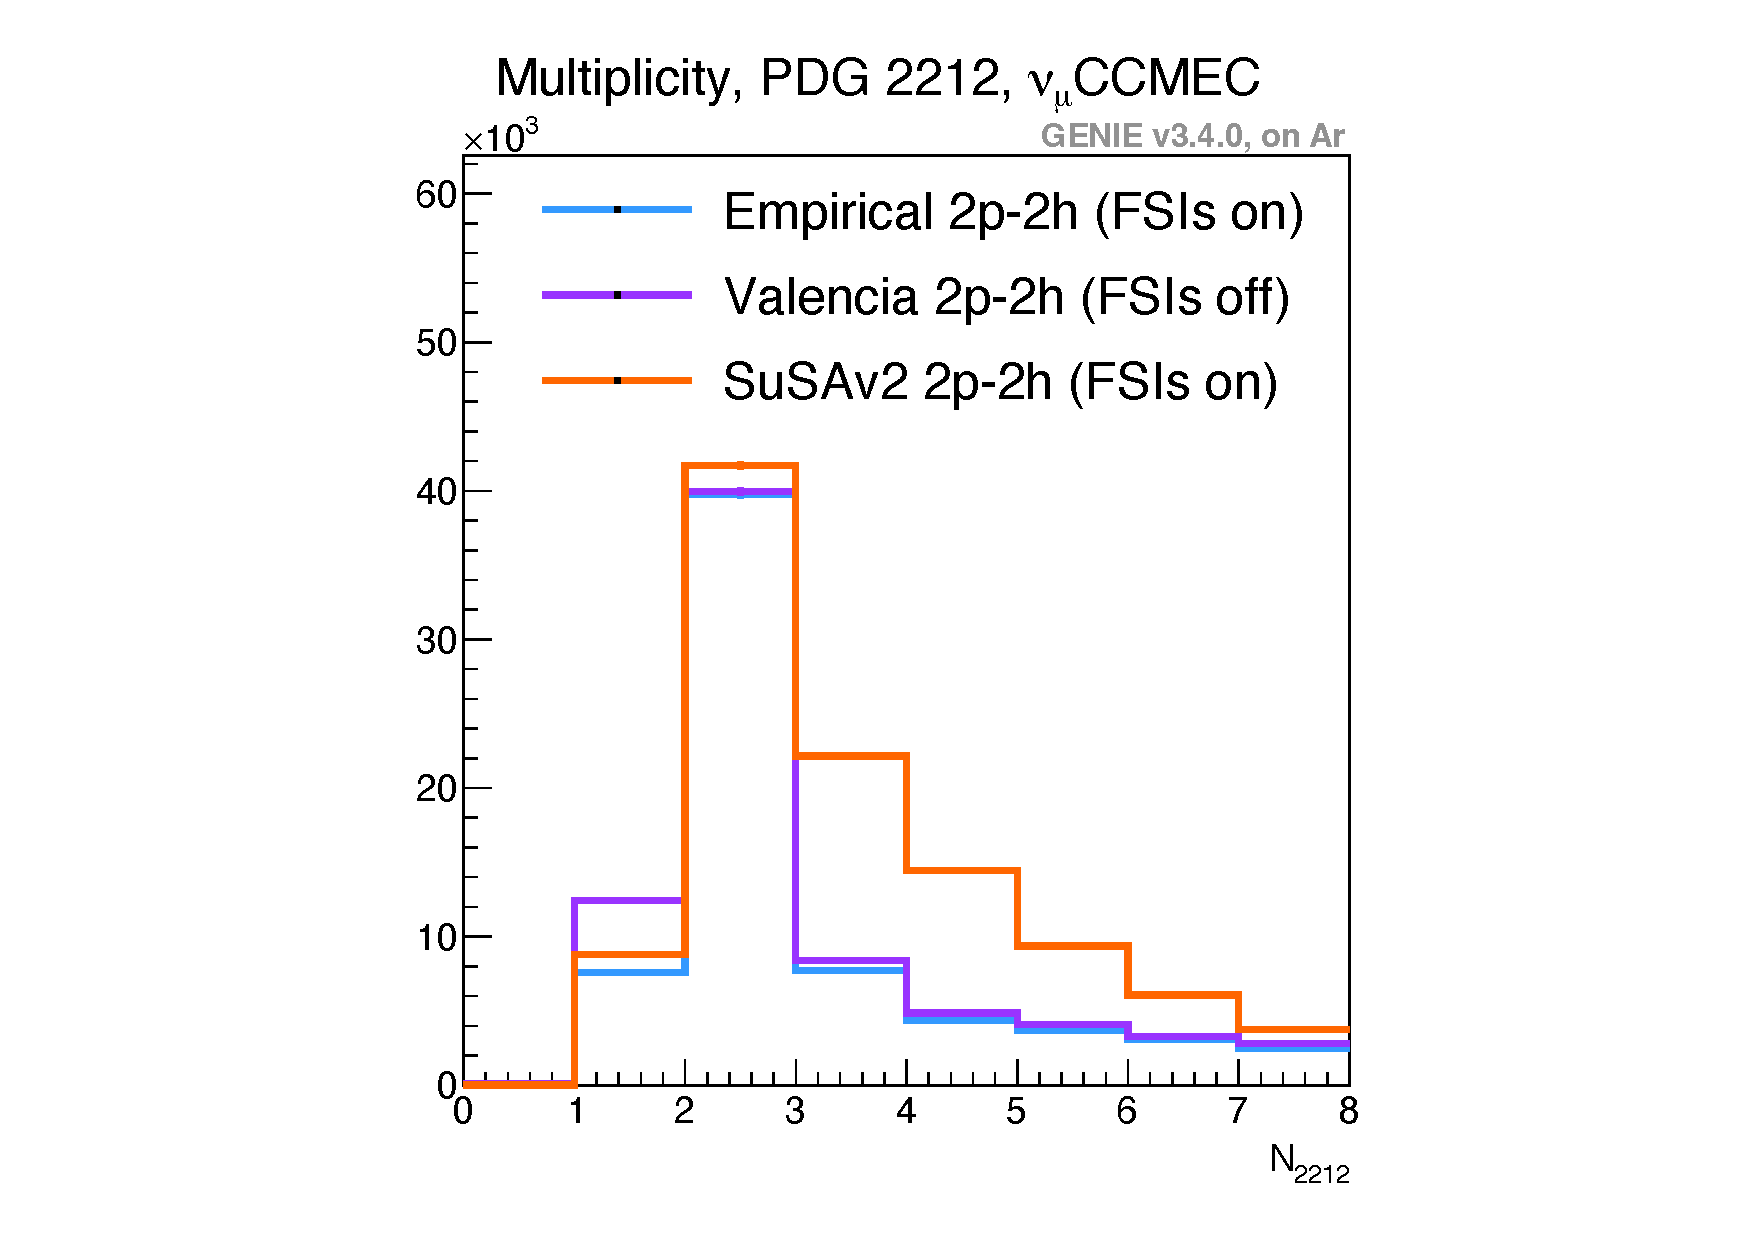
\includegraphics[width=\textwidth]{figures/postFSIs/1DComp_mult_2212_14_ccmec_multp_edited.pdf}
%        \vspace{-2.mm}
%    \caption{}
	\label{set2_b}
    \end{subfigure}
     %\vspace{-8mm}
 \begin{subfigure}[b]{.325\textwidth}
%        \includegraphics[width=\textwidth]{figures/1DComp_ErecAbsBias_14_ccmec.pdf}
        %
\includegraphics[width=\textwidth]{figures/postFSIs/1DComp_LeadP_p_14_ccmec_edited.pdf}
        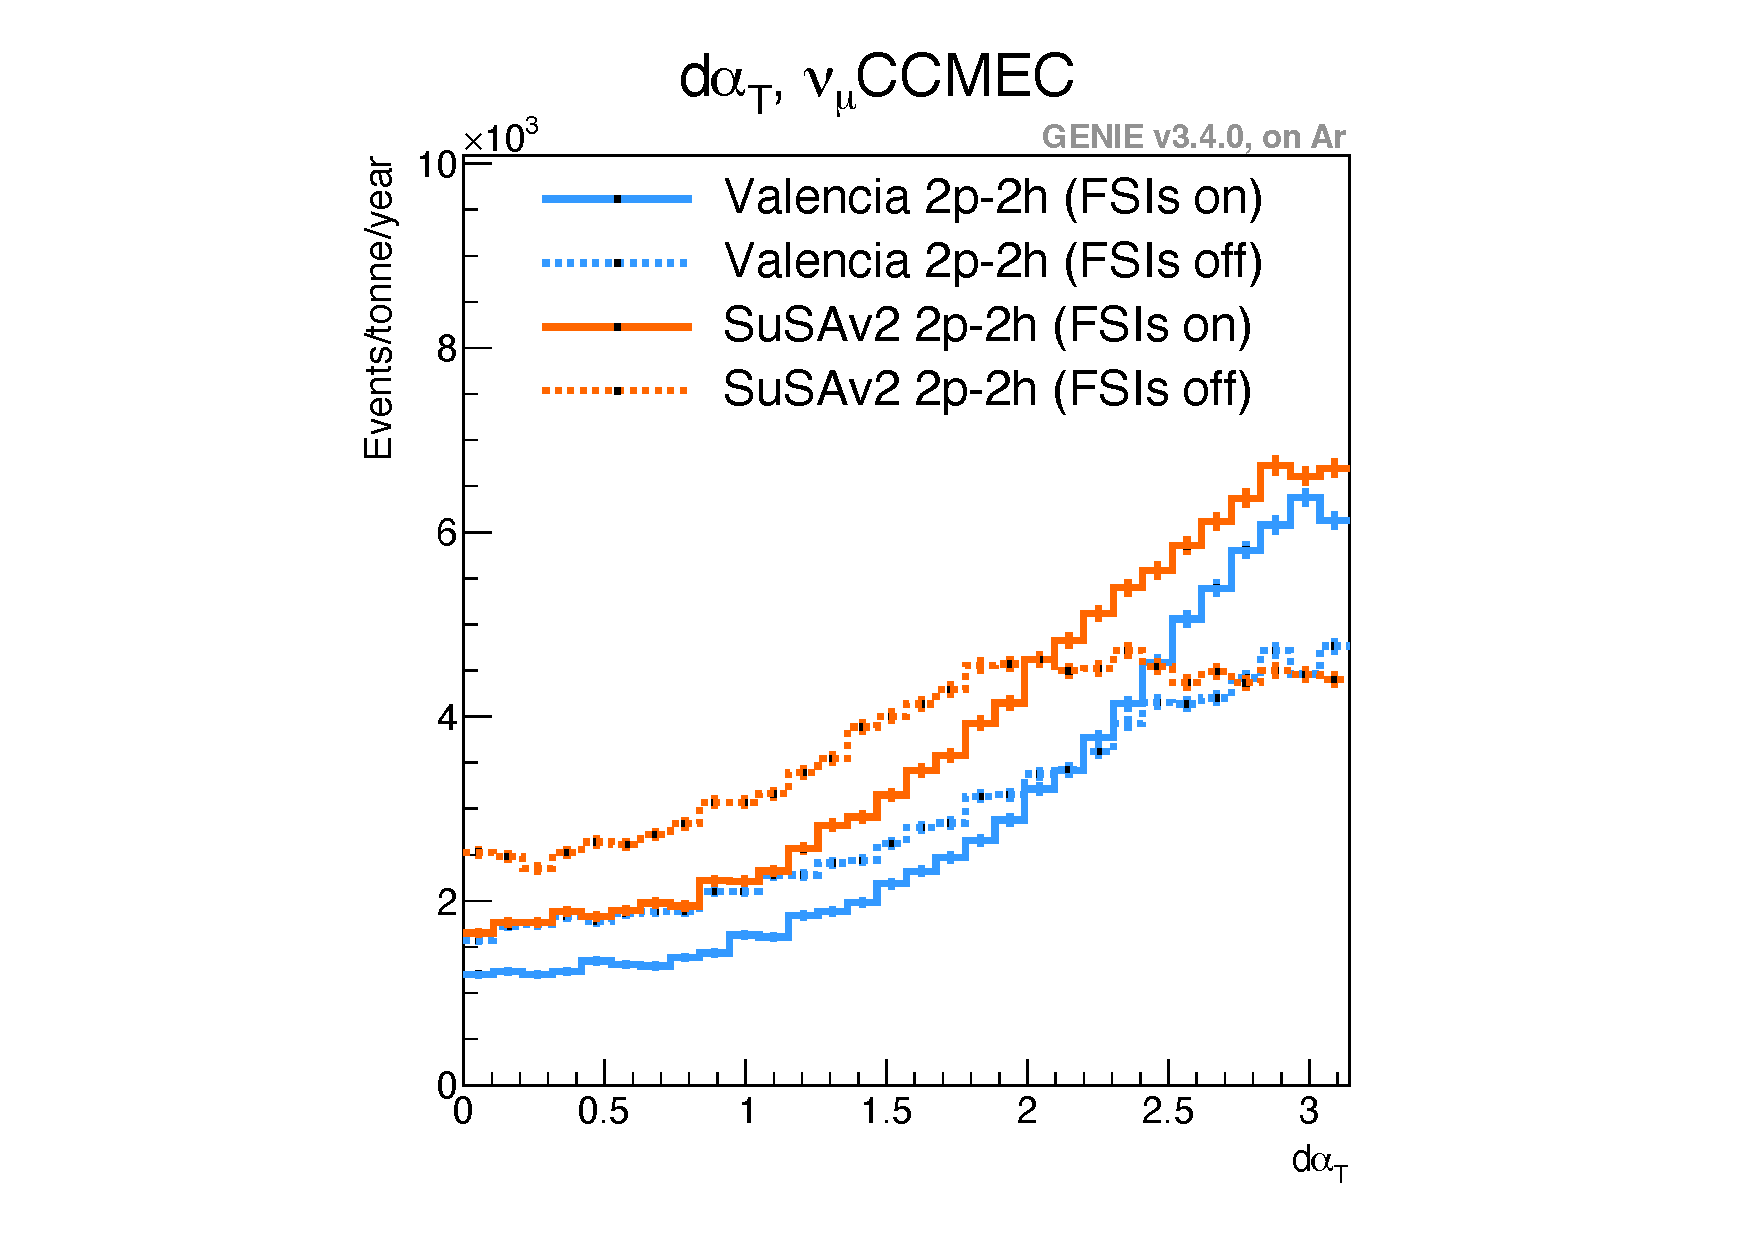
\includegraphics[width=\textwidth]{figures/FSI_vs_noFSI/1DComp_dat_14_ccmec.pdf}
%        \vspace{-6.mm}
%    \vspace{-2mm}
%	\caption{}
	\label{set2_c}
    \end{subfigure}
    \vspace{-6mm}
	\caption[]{Distributions of the number of events of GENIE-generated muon neutrino CC interactions on argon as a function of (left) the absolute reconstructed neutrino energy bias, (middle) the proton multiplicity and (right) the leading proton momentum.\vspace{-2mm}}
	\label{set2_plots}
\end{figure}
%
In \Cref{set2_plots} (left), one can observe a clear separation between the distributions of the Empirical and SuSAv2 \acrshort{cc} \acrshort{2p2h} models. Considering the neutrino energy bias $E_\nu = E_\text{reco} - E_\text{true}$ in an experiment like DUNE gives insight on choosing the right uncertainty model, such that the measurement of the oscillation parameters is not biased in case the wrong model is chosen, in which case nature could be closer to one of the other models. Regarding the proton multiplicity shown in \Cref{set2_plots} (middle), while the Empirical and Valencia model make rather similar predictions, the SuSAv2 model stands out in a way that could be potentially observed in an experiment like \acrshort{dune}. %One can also observe differences in the leading proton momentum distribution in \Cref{set2_c} between the three models.
%
Although the event weights are constructed such that their average weight $\langle w \rangle = 1$, this does not imply that the average weight is equal to unity within every bin of a given observable. For a weight $w(\theta)$ depending on a kinematic variable $\theta$, the average weight per bin for an observable $x$ is determined by the conditional distribution $P(\theta \mid x)$, which describes how $\theta$ is distributed among events in that bin. Consequently, only if $\theta$ is uncorrelated with $x$, such that $P(\theta \mid x) = P(\theta)$, does the average weight remain unity in each bin and the observable remains unchanged. Otherwise, deviations from unity lead to distortions of the $x$-distribution.

\subsection{New Systematic Uncertainty Parameters} \label{set3}
%Reweighting plots (Norm, shape ..., maybe show one hadron and muon variable, only if measure muon or proton can measure difference, PN dials apply to hadronic side, able to measure it in DUNE)
%energy bias plot, Proton KE or leading momentum, lepton momentum easy to measure, multiplicity proton,
%\subsection{Parameter Dials} \label{systematic_parameters}
In the following, I am introducing new systematic parameters with various numbers of tweaking dials, to account for uncertainties in the modelin of \acrshort{2p2h} interactions. These parameters were further developed from the ones presented in \cite{PhysRevD.105.072001} in order to obtain robust uncertainty estimates for future oscillation and cross-section analyses in \acrshort{dune}. The nominal base model prediction in the \acrshort{2p2h} channel is the SuSAv$2$ model. However, the development of the parameters presented in this section may be used for any experiment with the \acrshort{2p2h} Valencia, SuSAv$2$ or Martini et al. model as their central value prediction. The following plots were generated using the GENIE Reweight product \cite{web:genie_reweight} and show tweak dial variations with respect to four systematic parameters, i.e. $\verb!NormCCMEC!$ (\cref{sec:normccmec}), $\verb!DecayAngMEC!$, $\verb!DecayAng2MEC!$ and $\verb!DecayAngMECLegendre!$  (\cref{sec:decayangmec}), $\verb!FracPN_CCMEC!$ (\cref{sec:fracpnccmec}) and $\verb!XSecShape_CCMEC!$, $\verb!XSecShape_CCMEC_Empirical!$, $\verb!XSecShape_CCMEC_Martini!$ (\cref{sec:xsecshapeccmec}) and $\verb!EnergyDependence_CCMEC!$ (\cref{sec:edep_ccmec}).

\subsection{Normalisation Variation} \label{sec:normccmec}
%\paragraph{Normalisation Variation}
In order to evaluate uncertainties associated with the normalisation of a \acrfull{mc} predicted physical quantity $P$, a systematic parameter $x_P$ is introduced. This allows variations of $P$ with estimated standard deviation $\delta P$ in terms of $x_P$ and evaluate an event weight as a function of $x_P$. Tweaking $x_P$ may then modify the corresponding $P$ according to \cite{Andreopoulos:2009rq}
%
\begin{align} \label{eq:normalisation_tweak}
    P \longrightarrow P' = P\left( 1 + x_P \frac{\delta P}{P} \right) \ .
\end{align}
%
The parametrisation in \Cref{eq:normalisation_tweak} provides a general prescription for implementing normalisation-type uncertainties. Setting $x_P=0$ leaves $P$ unchanged from its nominal value. Tweaking $x_P$ by $\pm 1$ modifies the associated $P$ by $\pm \delta P$.


The normalisation parameter $\verb!NormCCMEC!$ is a specific realisation of this approach that changes the overall absolute normalisation of the \acrshort{cc} \acrshort{2p2h} cross section with no change in shape \cite{PhysRevD.105.072001}. In this case, the physics quantity $P$ corresponds to the cross-section $\sigma$ such that
%
\begin{align} \label{eq:normccmec_reweighting}
    \sigma \longrightarrow \sigma' = \sigma \left( 1 + x_\sigma^\text{NORMCCMEC} \cdot \frac{\delta \sigma}{\sigma} \right) \ \text{.}
\end{align}
%
\Cref{eq:normccmec_reweighting} results in a constant event weight across phase space and therefore corresponds to a uniform rescaling of the event rate without modifying the shape of kinematic distributions. A parameter value of $0$ corresponds to the default normalisation of \acrshort{cc} kinematic variable distributions of \acrshort{2p2h} interactions in \acrshort{genie}. Setting a positive value increases the average cross section, whereas a negative value decreases it. The effect of varying the $\verb!NormCCMEC!$ tweak dial $x_\sigma^\text{NORMCCMEC}$ on the leading proton momentum distribution for the Valencia, SuSAv2 and Martini et al. models is shown in \Cref{fig:normccmec}.
\iffalse
%
\begin{figure}[htb!]
	\begin{subfigure}[b]{.33\textwidth}
    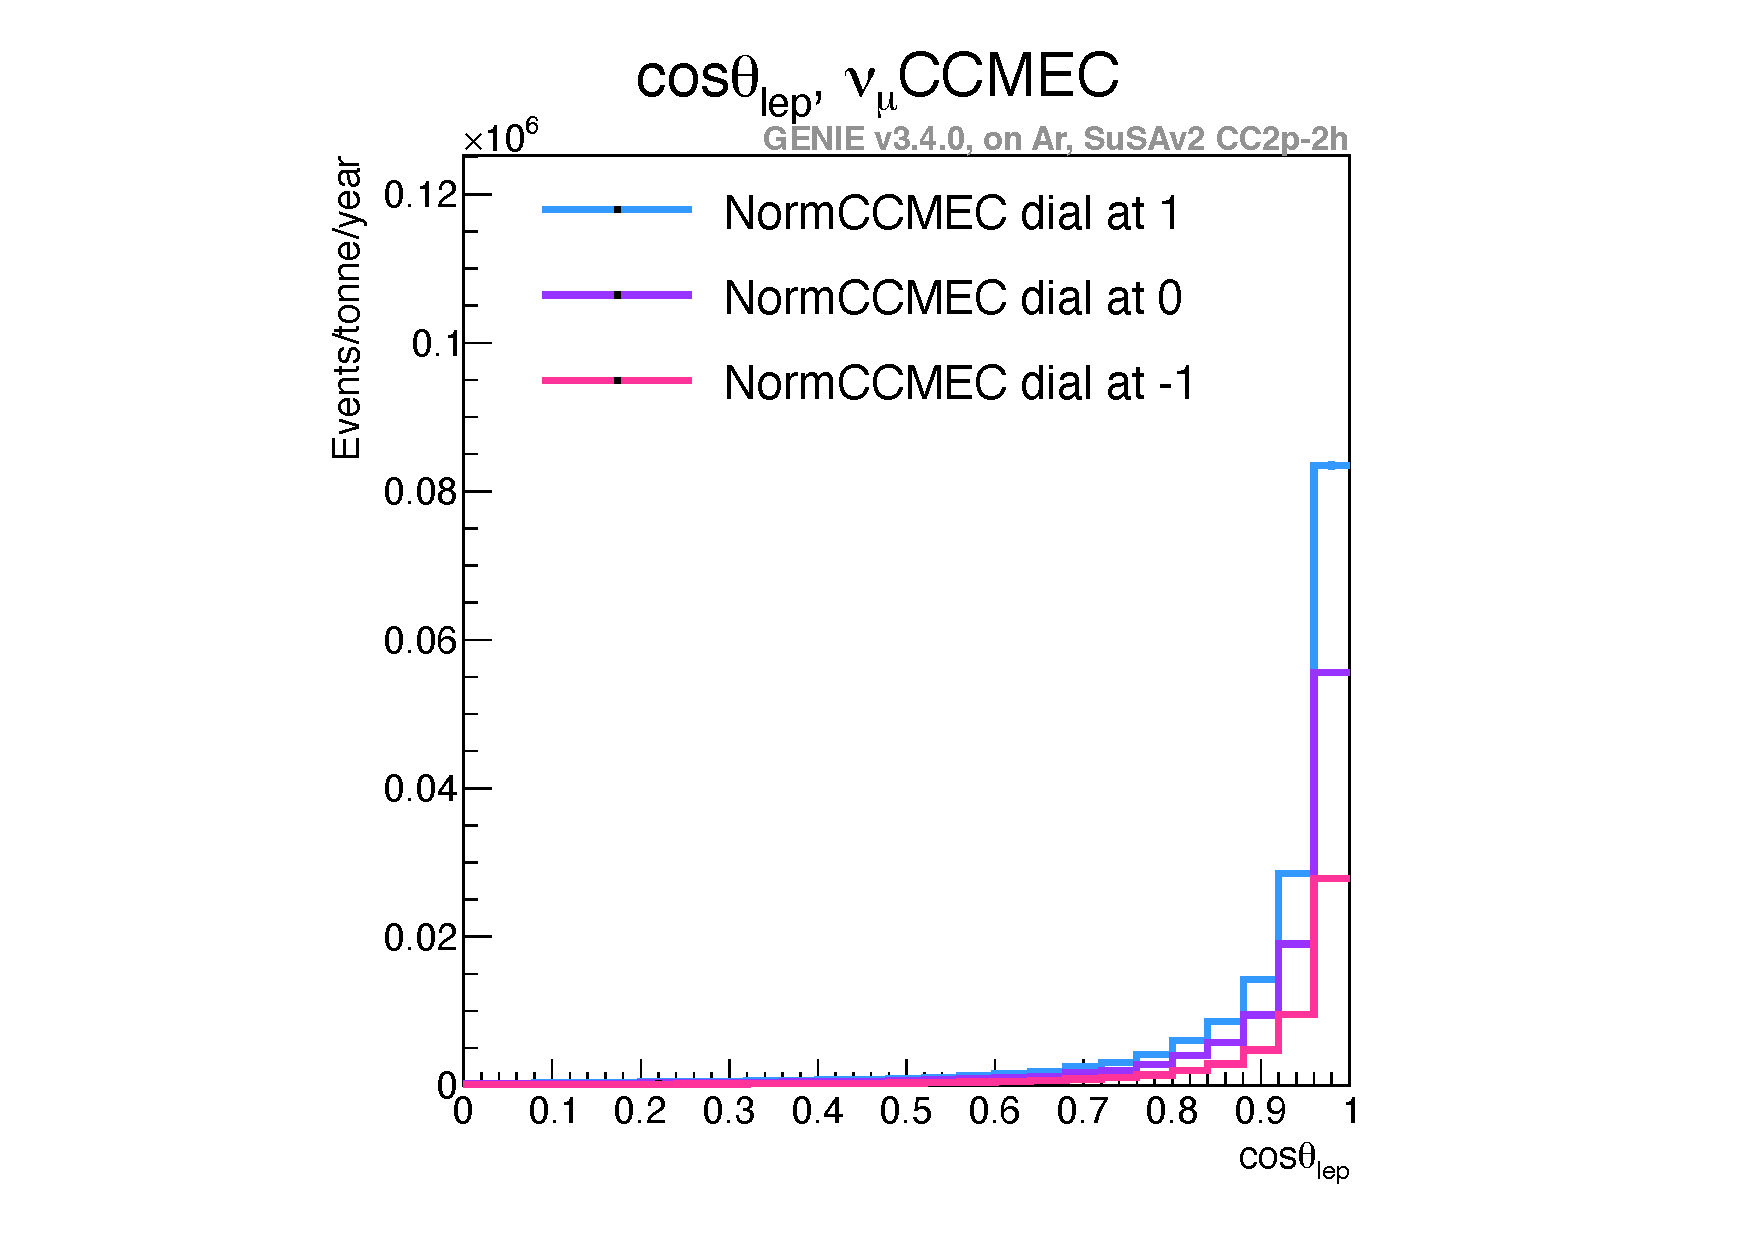
\includegraphics[width=\textwidth]{figures/Norm_CCMEC/1DComp_cosThetaLep_14_ccmec_edited.pdf}
	\label{normccmec_a}
    \end{subfigure}
	\begin{subfigure}[b]{.32\textwidth}
    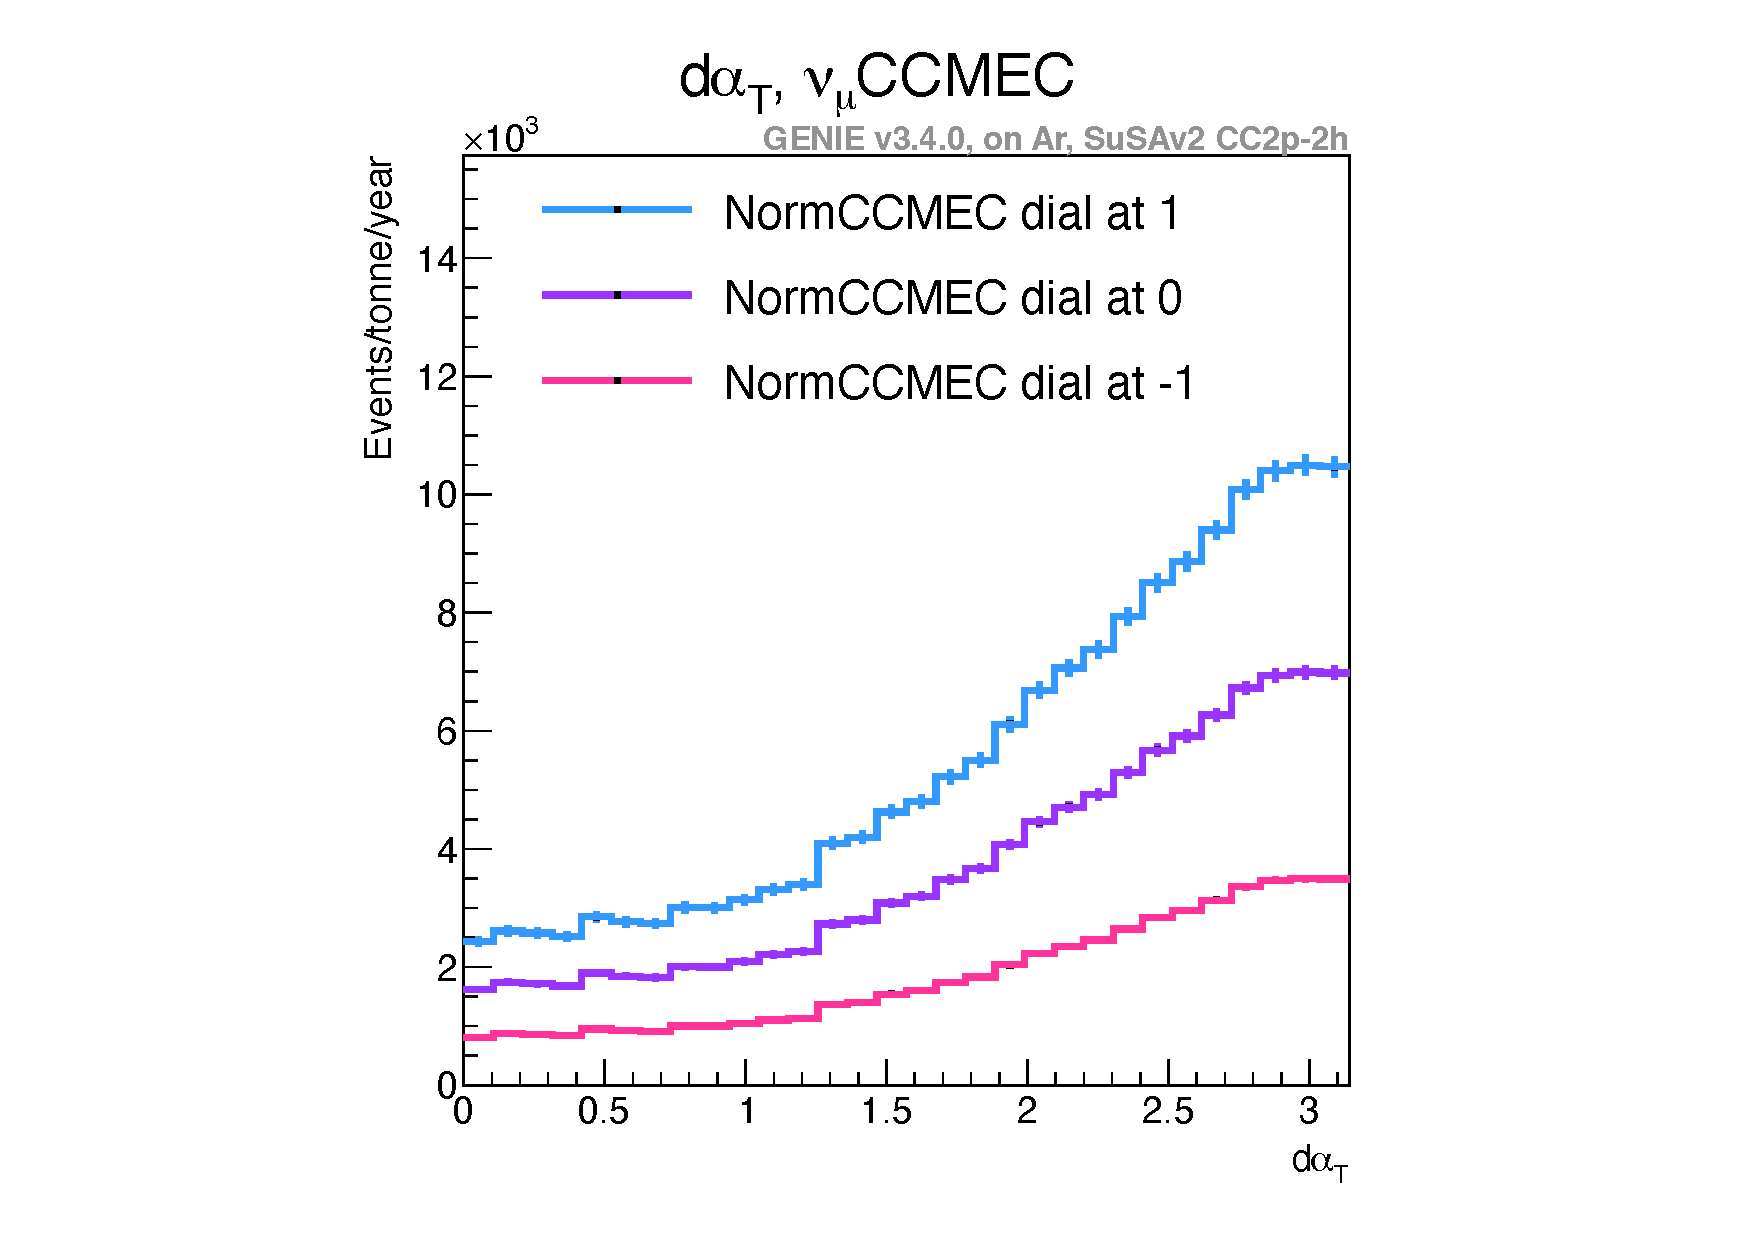
\includegraphics[width=\textwidth]{figures/Norm_CCMEC/1DComp_dat_14_ccmec_edited.pdf}
	\caption{}
	\label{normccmec_b}
    \end{subfigure}
	\begin{subfigure}[b]{.32\textwidth}
    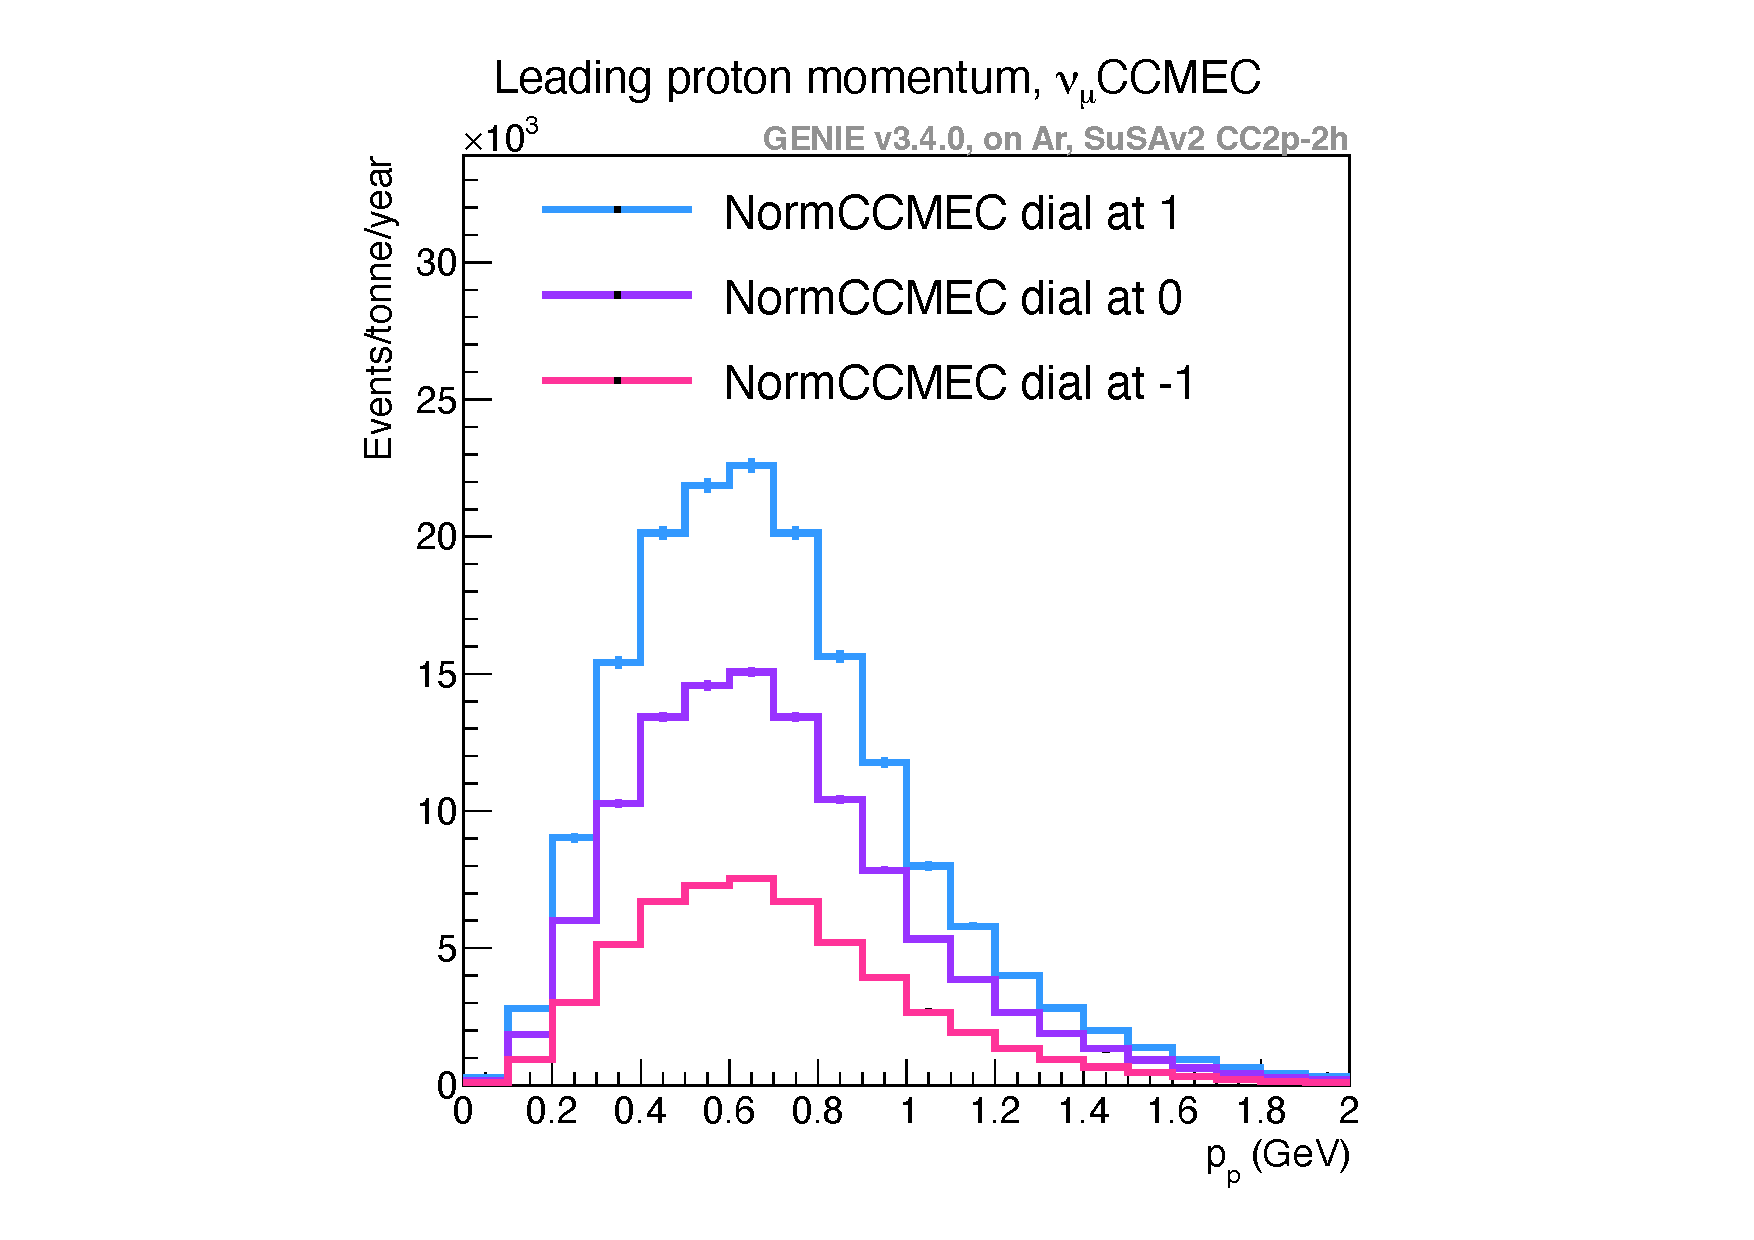
\includegraphics[width=\textwidth]{figures/Norm_CCMEC/1DComp_LeadP_p_14_ccmec_edited.pdf}
	\label{normccmec_c}
    \end{subfigure}
    \vspace{-6mm}
	\caption[]{NormCCMEC dials for the (left) lepton kinematic $\cos(\theta)_\text{lep}$, (middle) the hadron kinematic variable $p_p$ and (right) the transverse-kinematic angular imbalance $\mathrm{d}\alpha_T$.}
	\label{normccmec}
\end{figure}
%
\fi
%
%
    \begin{figure}[H]
	\centering
	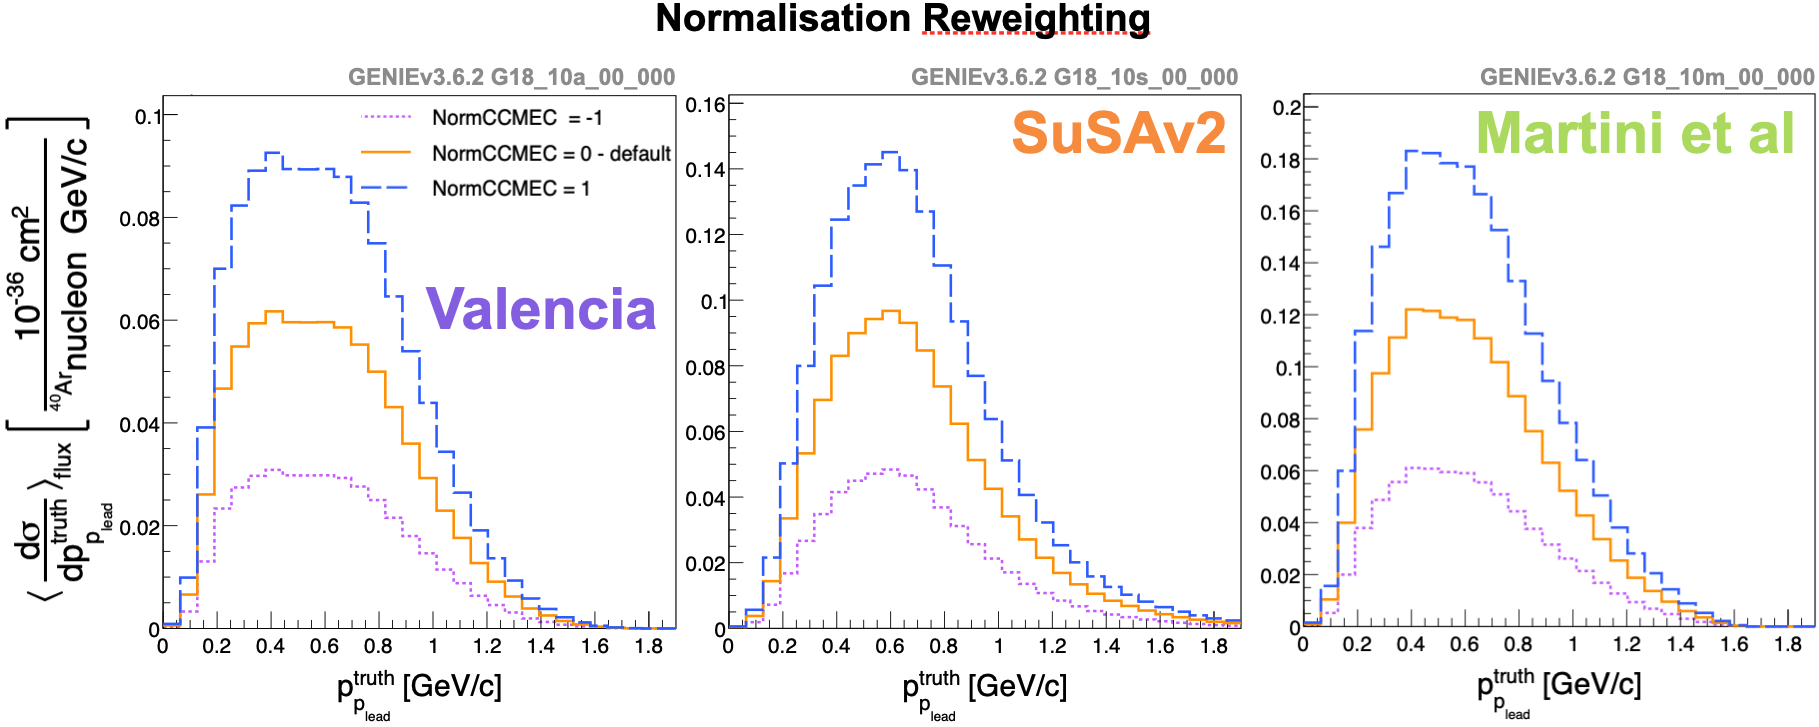
\includegraphics[width=\textwidth]{figures/Norm_CCMEC/normccmec.png}
	\caption[Normalisation Parameter]{Normalisation Parameter.}
	\label{fig:normccmec}
    \end{figure}
%
For all three input models, the tweak dial variations of the $\verb!NormCCMEC!$ parameter changes the overall normalisation with respect to the central value configuration and leaves the shape of the distributions unchanged.

\subsection{Nucleon Angular Distribution} \label{sec:decayangmec}
A slightly more complicated parameter is the $\verb!DecayAngMEC!$ parameter that modifies the angular dependency of the struck nucleon pair exiting the neutrino-interaction vertex. 
%So here I'm showing the, uh, a scatter of a neutrino of a NP pair, given rise to two nucleons in the final state. And again, redrawing this part of the image here. One can Lawrence boost this alongside this vector to get the two nucleons in the back to back frame. And then the angle this is about is this angle between the nucleon momentum and this leptonic three momentum transfer in the two nucleons center of mass frame. This is quite a complicated definition of this angle. So let's try to get some intuition on that. 
In the default model predictions of all \acrshort{2p2h} models currently implemented in \acrshort{genie}, the angular distribution of the outgoing nucleon pair is isotropic in their rest frame, as it can be seen in the flat default predictions shown in Figs. (\ref{fig:decayangmec_original})-(\ref{fig:decayangmec_legendre_valencia_martini}). This is due to the fact that all \acrshort{2p2h} models implemented in GENIE are inclusive, meaning that they only provide predictions for the outgoing lepton kinematics \cite{Gran:2013kda}. The detailed kinematics of the outgoing nucleons are not determined by the underlying interaction model and are instead generated using additional assumptions within \acrshort{genie}. In the \acrshort{genie} simulation, a two-nucleon hadronic final state is generated using an approximate approach known as the nucleon cluster model \cite{Katori:2013eoa}. In this framework, the leptonic four-momentum transfer is assigned to a correlated pair of nucleons, which are sampled independently from the nuclear ground-state distribution into one single object. The subsequent decay of this nucleon pair is then simulated to produce two outgoing nucleons. This nucleon-cluster decay is assumed to be isotropic in the rest frame of the nucleon pair \cite{PhysRevD.105.072001}. \Cref{fig:decayangmec_explanation} is an illustration of $\theta_\text{DecayAngMEC}$.
%
    \begin{figure}[H]
	\centering
	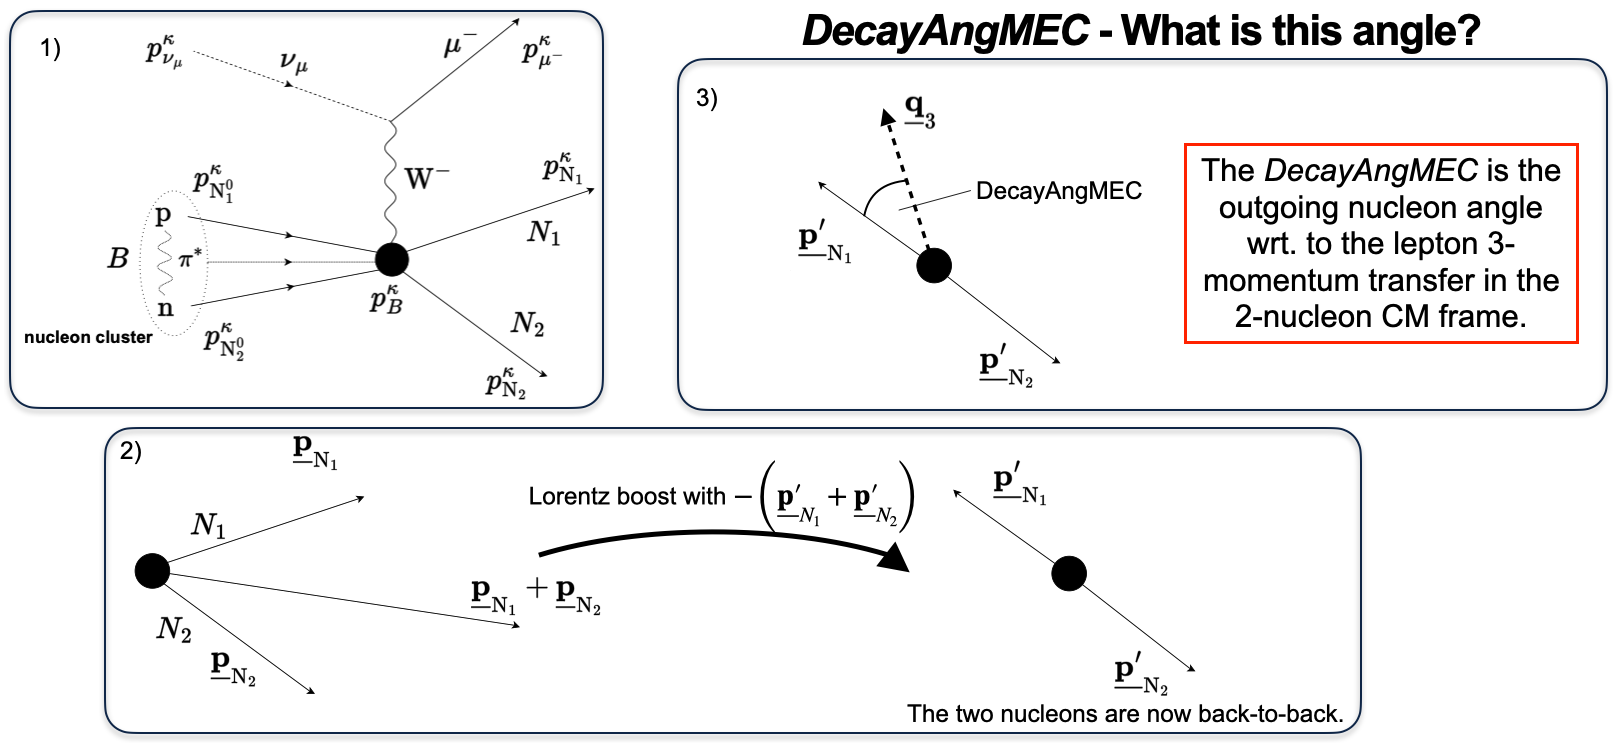
\includegraphics[width=\textwidth]{figures/DecayAngMEC/decayangmec_explanation.png}
	\caption[DecayAngMEC – What is this Angle?]{Illustration of the angle $\theta_\text{DecayAngMEC}$ between the $3$-momentum transfer and one of the nucleon's momenta in the boosted \acrshort{cm} frame.}
	\label{fig:decayangmec_explanation}
    \end{figure}
%
This ad-hoc assumption of an isotropic nucleon angular distribution, lacking firm theoretical justification, is challenged through dedicated reweighting variations via the $\verb!DecayAngMEC!$ parameter. In contrast to the normalisation variation via \Cref{eq:normccmec_reweighting}, other parameters such as the $\verb!DecayAngMEC!$ parameter modify the shape of kinematic distributions and lead to event weights that depend explicitly on the event kinematics. In such cases, the variation cannot be expressed as a modification of a single \acrshort{mc}-predicted physical parameter $P$ as in \Cref{eq:normalisation_tweak}. Instead, a systematic parameter $x^\text{DecayAngMEC}_P$ is introduced to directly modify the underlying kinematic distributions through event reweighting.






The \acrshort{cc} \acrshort{2p2h} models described above are inclusive meaning that they only predict the particle kinematics of the outgoing lepton. In the so-called nucleon cluster model \cite{10.1063/1.4919465}, a bound pair of two nucleons is sampled independently from the nuclear ground state distribution and treated as a single object. The leptonic $4$-momentum transfer of the neutrino interaction is imparted on this two-nucleon hadronic final state which then decays to two outgoing nucleons. In the current GENIE \acrshort{cc} \acrshort{2p2h} implementations, the decay angle of these two outgoing nucleons in their rest frame follows an isotropic angular distribution. However, this assumption may be challenged by the $\verb!DecayAngMEC!$ parameter which introduces an angular dependence on the final-state particle kinematics. Hereby, a \acrshort{cc} \acrshort{2p2h} $\verb!DecayAngMEC!$ dial at $0$ resembles the default isotropic distribution, whereas a dial at $1$ yields an angular dependence proportional to $\cos^2(\theta)$ (as a rather anisotropic distribution), where $\theta$ is measured with respect to the $3$-momentum transfer $\mathbf{q}$. Values in between $0$ and $1$ correspond to linear interpolations between these two distributions \cite{PhysRevD.105.072001}.


The tuning of the $\verb!DecayAngMEC!$ %as well as the $\verb!FracPN_CCMEC!$ 
systematic parameter have relatively small effects on the distributions shown in \Cref{decayangmec}. However, there are subtle differences in the distributions for the decay angle between the struck nucleons in dependence on whether the final-state of the interaction was a np- or pp-pair (see \Cref{decayangmec} (left) and (middle)). The change of the leading proton momentum distribution in \Cref{decayangmec} (right) is modest, as it would be expected, since this dial represents a physical effect regarding the outgoing nucleons only.  %Though a combined measurement of this leptonic kinematic variable distribution with the leading proton momentum distriblution may allow one to find a region of phase space that provides discrimination potential between the three models. 

\paragraph{Decay-Angle-MEC Parameter – 1 Tweak Dial}
The parameter \verb!DecayAngMEC! was originally developed by MicroBooNE \cite{PhysRevD.105.072001} and provides a concrete example of a shape variation parameter. It alters the angular distribution of the two outgoing nucleons in \acrshort{cc} \acrshort{2p2h} interactions away from being isotropic by interpolating between this isotropic distribution and an alternative model proportional to $\cos^2(\theta_\text{DecayAngMEC})$, where $\theta_\text{DecayAngMEC}$ denotes the emission angle of one nucleon with respect to the $3$-momentum transfer $\mathbf{q}_3$ in the two-nucleon centre-of-momentum frame, as illustrated in \Cref{fig:decayangmec_explanation}.
The corresponding event weight is given by
%
\begin{align} \label{eq:decayangmec_weight}
    w^\text{DecayAngMEC} (\theta) = 3\,x_\theta\,\cos^2(\theta) + \left(1 - x_\theta\right) \ ,
\end{align}
%
where $x_{\theta}^\text{DecayAngMEC} = 0$ corresponds to the nominal isotropic distribution and $x_{\theta}^\text{DecayAngMEC} = 1$ ($-1$) corresponds to an angular dependence proportional to the alternative $\cos^2(\theta)$ ($-\cos^2(\theta)$) distribution, as it is shown in \Cref{fig:decayangmec_original}.
%
    \begin{figure}[htb]
	\centering
	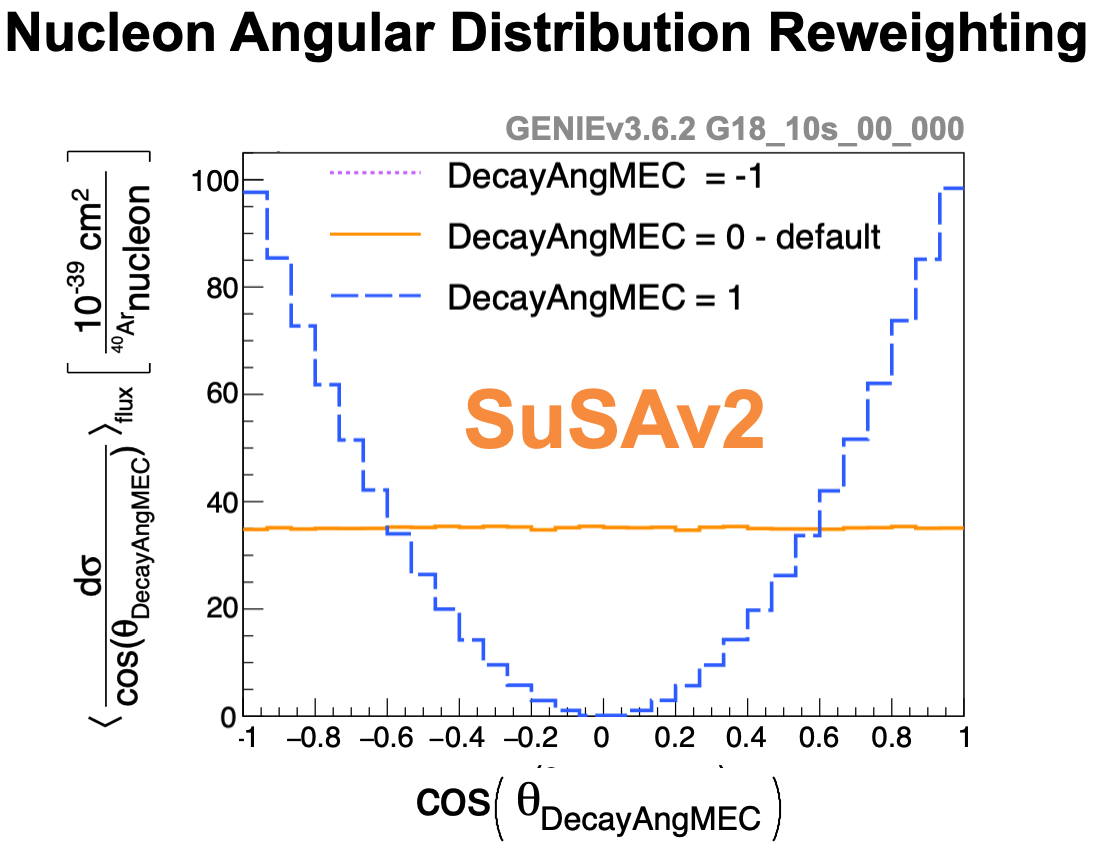
\includegraphics[width=\textwidth]{figures/DecayAngMEC/decayangmec_original.png}
	\caption[Original Nucleon Angular Distribution Parameter Parameter]{Original Nucleon Angular Distribution Parameter Parameter.}
	\label{fig:decayangmec_original}
    \end{figure}
%
Unlike normalisation variations, the weight in \Cref{eq:decayangmec_weight} depends explicitly on the event kinematics, i. e. $\theta_\text{DecayAngMEC}$, and therefore modifies the shape of observables. The impact of this variation on a given observable $x$ depends on the correlation between $x$ and the decay angle $\theta_\text{DecayAngMEC}$. As a result, observables that are weakly correlated with $\theta_\text{DecayAngMEC}$, such as the muon momentum $p_\mu$, are largely unaffected, while the $\cos(\theta_\text{DecayAngMEC})$ observable exhibit significant distortions.

As illustrated in \Cref{fig:decayangmec_original_exp_cos}, the effect of applying $w^\text{DecayAngMEC} (\theta)$ on the $\cos(\theta_\text{DecayAngMEC})$ distribution is an enhancement of events in the forward and backward scattering regions and a suppression of scattering at right angles. 
\iffalse
%
    \begin{figure}[H]
	\centering
	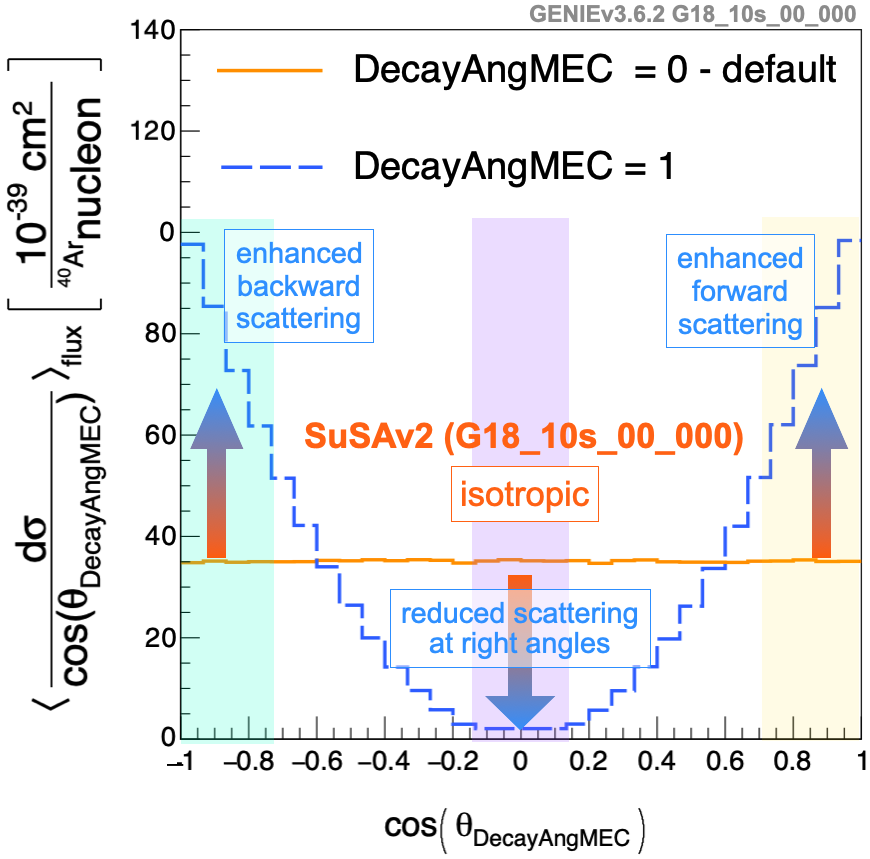
\includegraphics[width=\textwidth]{figures/DecayAngMEC/decayangmec_original_exp.png}
	\caption[Normalisation Parameter]{Normalisation Parameter.}
	\label{fig:decayangmec_original_exp}
    \end{figure}
%
\fi
%
    \begin{figure}[H]
	\centering
	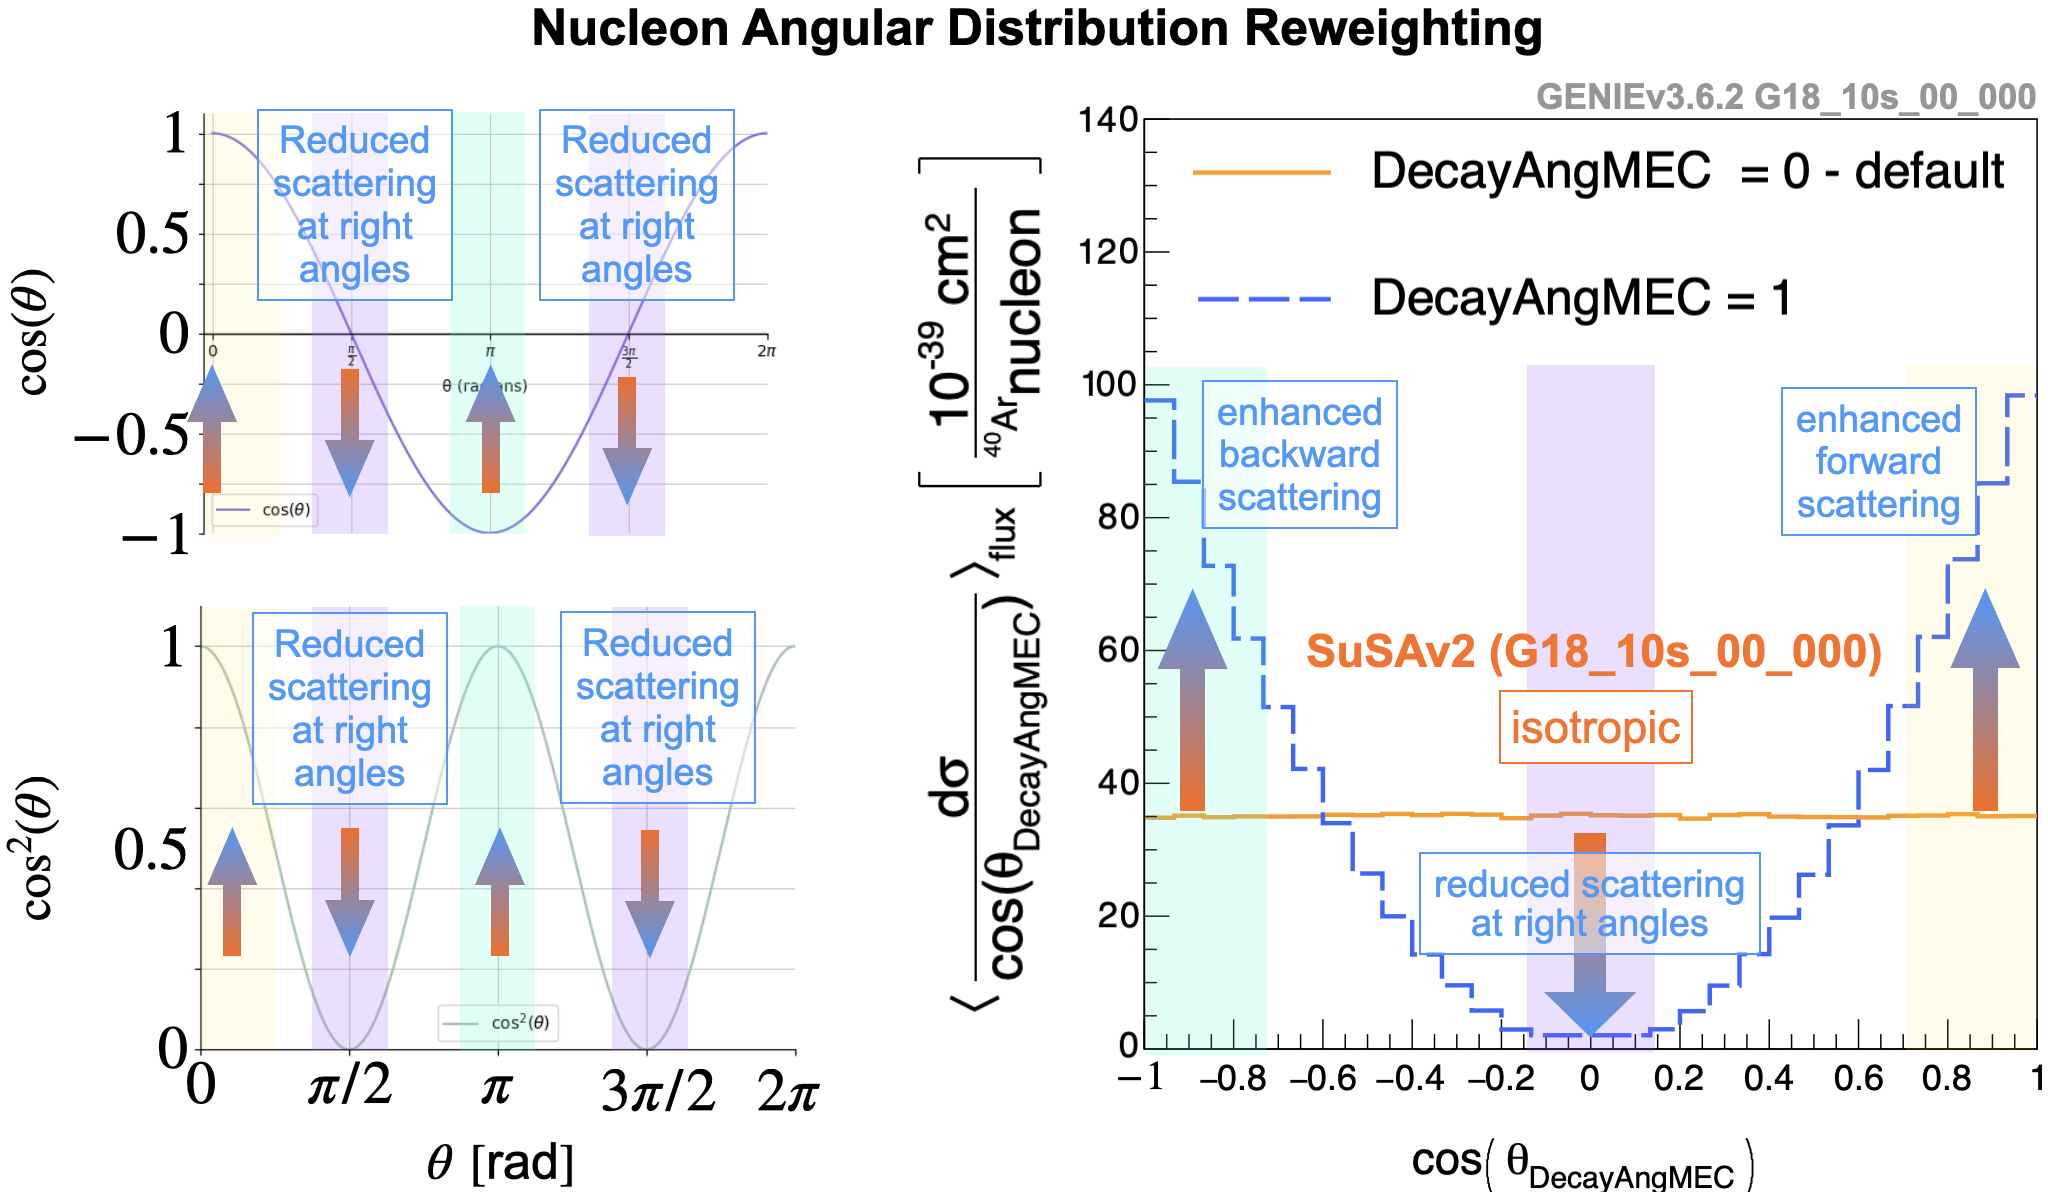
\includegraphics[width=\textwidth]{figures/DecayAngMEC/decayangmec_original_exp_cos.png}
	\caption[Illustration of Nucleon Angular Distribution Parameter]{Illustration of Nucleon Angular Distribution Parameter.}
	\label{fig:decayangmec_original_exp_cos}
    \end{figure}
%
Allowing $x_{\theta}^\text{DecayAngMEC} \in [-1,1]$ yields in the angular distributions for all three \acrshort{2p2h} models in \Cref{fig:decayangmec_modified_1twkdial}.
%
    \begin{figure}[H]
	\centering
	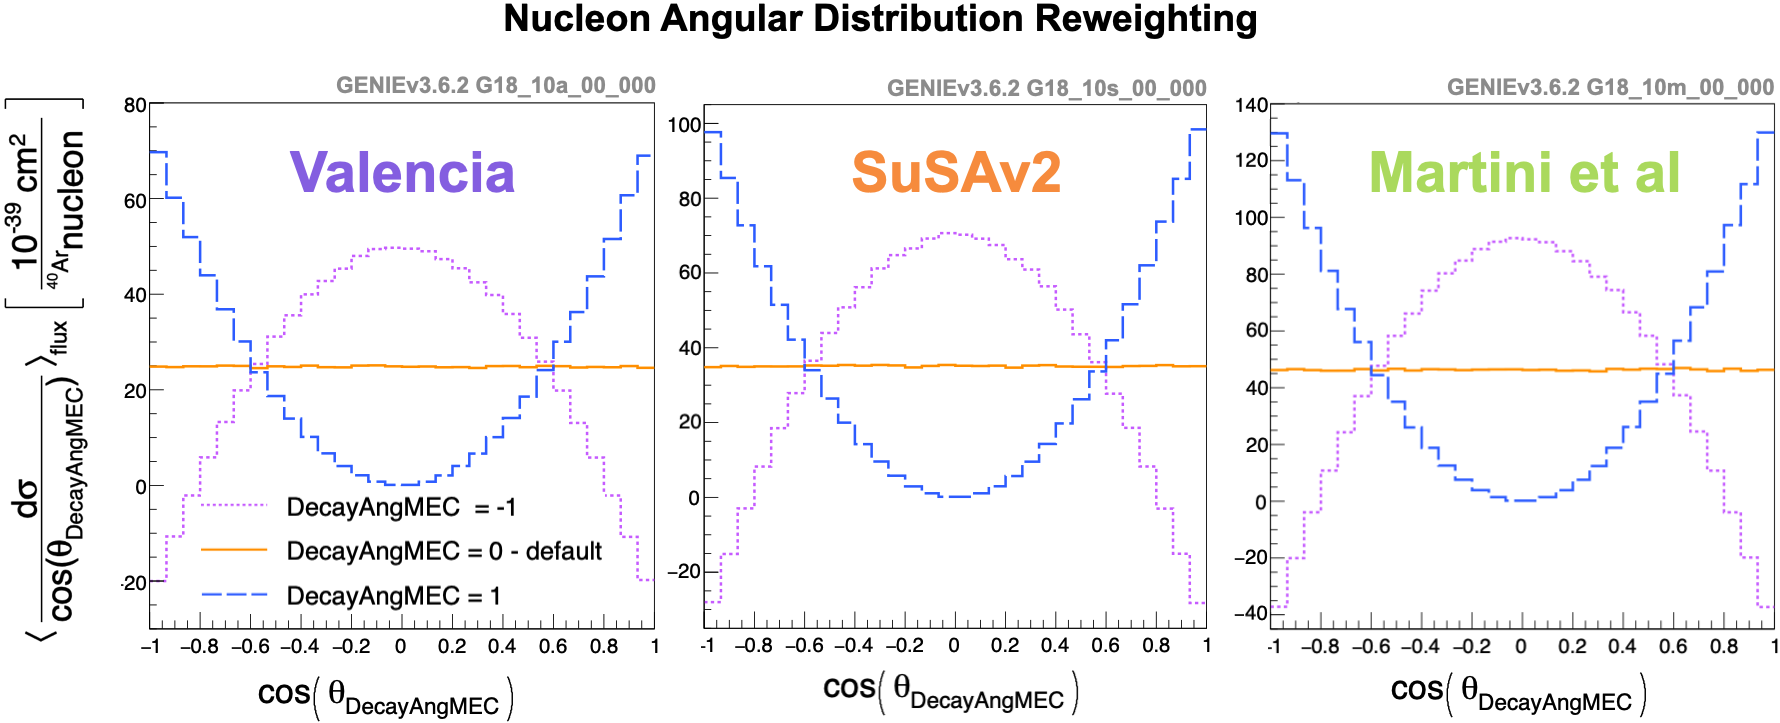
\includegraphics[width=\textwidth]{figures/DecayAngMEC/decayangmec_modified_1twkdial.png}
	\caption[Illustration of Nucleon Angular Distribution Parameter]{Illustration of Nucleon Angular Distribution Parameter.}
	\label{fig:decayangmec_modified_1twkdial}
    \end{figure}
%
This choice of changing the angular dependence in this way is not well physically motivated as the underlying physics of these outgoing nucleon directions is challenging to describe. In order to accommodate this difficulty, another dial was implemented that changes the frequency of the distribution (see \cref{norm_angle_params}). 

\paragraph{DecayAngleMEC Parameter with Two Tweak Dials}
In order to allow additional freedom in the modelling of the nucleon angular distribution, the single-dial \verb!DecayAngMEC! weight in \Cref{eq:DecayAngMECLegendre_weight} is extended to include a second tweak dial. The modified weight is defined as
%
\begin{align} \label{eq:decayang2mec_weight}
    w^\text{DecayAng2MEC} (\theta) = \frac{ 3\,x_{\theta_1}\,\cos^2(x_{\theta_2} \cdot \theta) + \left(1 - x_{\theta_1}\right) }{1 - x_{\theta_1} + 3x_{\theta_1}\cdot (1/2 + (1+cos(2\pi\cdot x_{\theta_2}))/(4\cdot (1- 4\cdot \left(x_{\theta_2}\right)^2)))} \ ,
\end{align}
%
allows more freedom due to a second tweak dial $x_{\theta_2}^\text{DecayAng2MEC}$ to vary the frequency. In order to preserve the cross-section normalisation the modified, weight has to be divided by the denominator in \Cref{eq:decayang2mec_weight}. The resulting reweighted distributions are shown in Figs. \ref{fig:decayangmec_modified_2twkdials_susav2} and \ref{fig:decayangmec_modified_2twkdials_valencia_martini}
%
    \begin{figure}[htb]
	\centering
	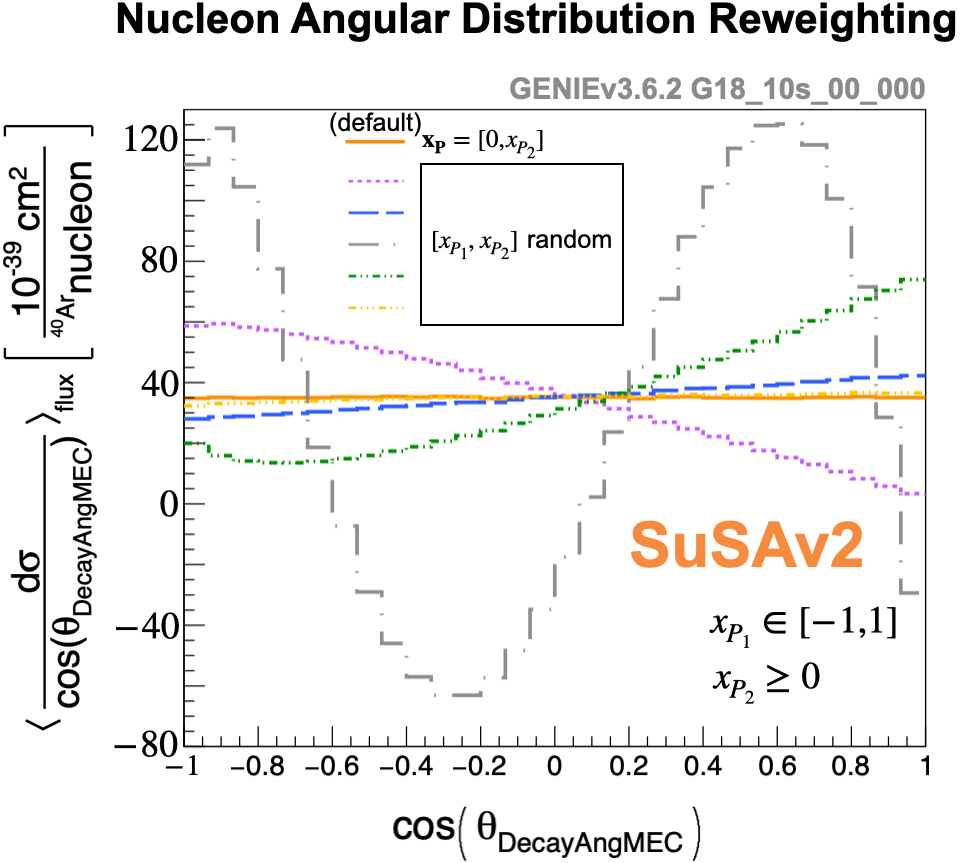
\includegraphics[width=0.8\textwidth]{figures/DecayAngMEC/decayangmec_modified_2twkdials_susav2.png}
    \caption[Nucleon Angular Distribution Parameter with Two Tweak Dials – SuSAv2]{
    Nucleon Angular Distribution Parameter with Two Tweak Dials of the input SuSAv2 model. Effect of the two-dial \texttt{DecayAng2MEC} reweighting on the nucleon angular distribution for the SuSAv2 \acrshort{cc} \acrshort{2p2h} model. The first tweak dial controls the strength of the angular deformation, while the second modifies the angular dependence.}
	\label{fig:decayangmec_modified_2twkdials_susav2}
    \end{figure}
%
%
    \begin{figure}[hbt]
	\centering
	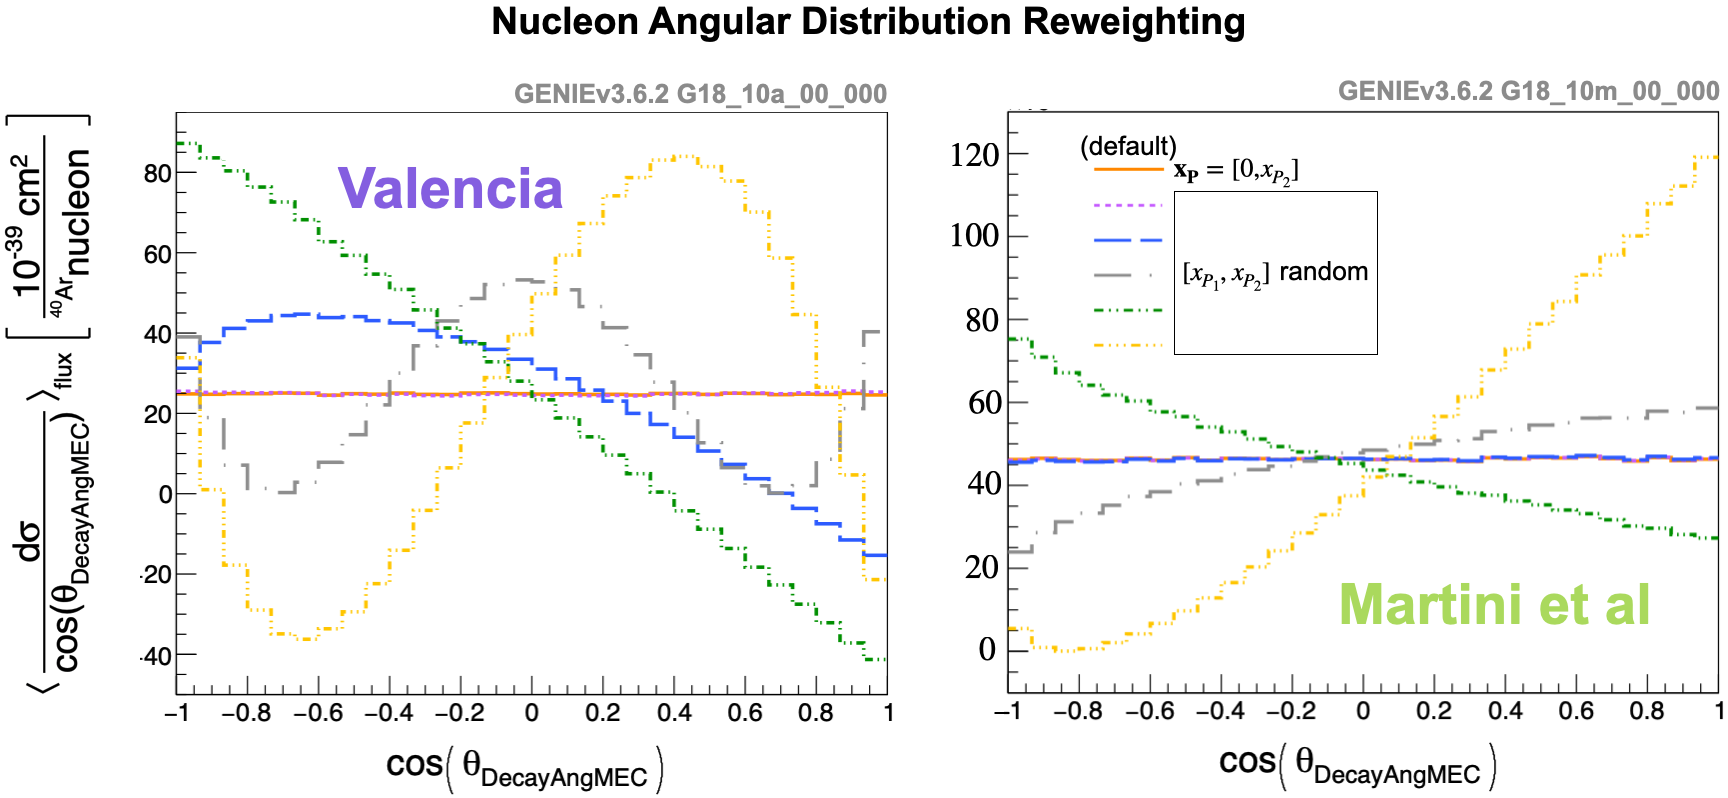
\includegraphics[width=\textwidth]{figures/DecayAngMEC/decayangmec_modified_2twkdials_valencia_martini.png}
    \caption[Nucleon Angular Distribution Parameter with Two Tweak Dials – Valencia and Martini et al]{
    Nucleon Angular Distribution Parameter with Two Tweak Dials of the input Valencia and Martini et al. models. Effect of the two-dial \texttt{DecayAng2MEC} reweighting on the nucleon angular distribution for the Valencia and Martini \acrshort{cc} \acrshort{2p2h} models. The event weight is computed according to \Cref{eq:decayang2mec_weight}.}
	\label{fig:decayangmec_modified_2twkdials_valencia_martini}
    \end{figure}
%
Here, $x_{\theta_1}$ controls the strength of the deviation from the nominal isotropic decay model, while \(x_{\theta_2}\) modifies the angular dependence of the anisotropic component. The denominator in \Cref{eq:decayang2mec_weight} ensures that the modified weight preserves the total cross-section normalisation, such that the reweighting changes only the shape of the angular distribution.

The resulting reweighted distributions are shown in \Cref{fig:decayangmec_modified_2twkdials_susav2,fig:decayangmec_modified_2twkdials_valencia_martini}.

\paragraph{Decay-Angle-MEC-Legendre Parameter – 6 Tweak Dials}
The default GENIE treatment of the two-nucleon decay in \acrshort{cc} \acrshort{2p2h} interactions assumes an isotropic angular distribution in the rest frame of the recoiling nucleon pair.
Since this ad-hoc assumption is not strongly constrained by theory, an additional shape uncertainty with increased flexibility is introduced. In general, an intuitive way to model such an uncertainty is to consider a set of physically motivated angular functions $f_i$ and form a linear combination of these functions,
%
\begin{align} \label{eq:func_linear_combination}
    f' = k \cdot f_0 + \sum^{N-1}_{i=1} (c_i \cdot f_i) \ \text{,}
\end{align}
%
where, for example $f_0$ corresponds to an isotropic component and the functions $f_i$ may represent alternative angular shapes, such as  forward-backward asymmetry or forward-peaked configurations. The coefficients $k, c_i$ determine the functions' relative contributions. In order to preserve the total normalisation, the coefficients are required to satisfy a constraint, which can be imposed through the explicit form of $k$.

In the present work, instead of using a set of specific angular distributions, the novel \verb!DecayAngMECLegendre_CCMEC! parameter modifies the angular dependence of the decay angle $\theta_\text{DecayAngMEC}$ (illustrated in \Cref{fig:decayangmec_explanation}) using a finite expansion in Legendre polynomials, which provides a more sophisticated method to estimate the uncertainty on the angular distribution of the two struck nucleons that exit the neutrino interaction vertex.

Legendre Polynomials provide a natural basis for angular distributions, because they form an orthogonal set on the interval $\cos(\theta_\text{DecayAngMEC}) \in [-1,1]$. They commonly appear in systems with spherical symmetry, for example in multipole or partial-wave expansions, as angular part of solutions to the Schr\"odinger equation and in the construction of spherical harmonics.
The Legendre polynomials are defined through Rodrigues' formula \cite{Rodrigues1816},
%
\begin{align} \label{eq:LegendrePoly_def}
    P_\ell (x) = \frac{1}{2^\ell \ell!} \frac{\text{d}^\ell}{\text{d}x^\ell} (x^2 - 1)^\ell \ \text{.}
\end{align}
%
The first six orders are
%
\begin{align} \label{eq:LegendrePoly_explicite}
    P_0 (x) &= 1 \\
    P_1 (x) &= x \\
    P_2 (x) &= \frac{1}{2} (3x^2 - 1) \\
    P_3 (x) &= \frac{1}{2} (5 x^3 - 3x) \\
    P_4 (x) &= \frac{1}{8} (35 x^4 - 30x^2 + 3) \\
    P_5 (x) &= \frac{1}{8} (63 x^5 - 70x^3 + 15x) \\
    P_6 (x) &= \frac{1}{16} (231 x^6 - 315x^4 + 105 x^2 - 5) \ \text{.} \\
\end{align}
%
The average value of the Legendre polynomials over the interval $[-1,1]$ is given by
%
\begin{align} \label{eq:LegendrePoly_avg}
    \frac{1}{2} \int_{-1}^1 P_\ell(x)\mathrm{d}x =
    \begin{cases}
        1 & \text{if } \ell = 0 \\
        0 & \text{if } \ell \geq 1 \text{.}
    \end{cases}
\end{align}
%
This property makes them particularly suitable for constructing shape variations that preserve the total normalisation for an initially isotropic distribution.

The weight $w^\text{DecayAngMECLegendre}$ can be written as a linear combination of the Legendre polynomials $P_\ell(\cos(\theta_\text{DecayAngMEC}))$ with coefficients $x_{\theta_\ell}$ that are summarised in the vector $\mathbf{x}_\theta = \{{x_{\theta_1}, x_{\theta_2}, x_{\theta_3}, x_{\theta_4}, x_{\theta_5}, x_{\theta_6}}\}$ and control the contribution of each Legendre mode. The modified cross section $\sigma'$ becomes
%
\begin{align} \label{eq:ansatz_DecayAngMECLegendre_weight}
    \sigma' = \left[ k \cdot w_0 + \sum^{N-1}_{\ell=1} (x_{\theta_\ell} \cdot w_\ell) \right] \sigma \ \text{.}
\end{align}
%
Here, $w_0$ corresponds to the constant isotropic component and $w_\ell$ denote the shape-varying angular components. The coefficients $k$ and $x_{\theta_\ell}$ enhance or diminish the $i$-th Legendre Polynomial and satisfy the normalisation constraint
%
\begin{align} \label{eq:norm_constraint_DecayAngMECLegendre}
    k = 1 - \sum^{N-1}_{\ell=1} x_{\theta_\ell} \ \text{.}
\end{align}
%
Since the average of each $P_\ell$ with $\ell \geq 1$ vanishes for an isotropic distribution in $\cos\theta_\text{DecayAngMEC}$ (\ref{eq:LegendrePoly_avg}), the global average of the weight remains unity,
%
\begin{align}
    \langle w^\text{DecayAngMECLegendre} \rangle = 1 \ ,
\end{align}
%
provided the nominal distribution is isotropic. The normalisation constraint handling the $0$-th order mode $P_0(\cos\theta_\text{DecayAngMEC})$ in \Cref{eq:norm_constraint_DecayAngMECLegendre} makes sure to preserve this property. Thus, this parameter changes the shape of the nucleon angular distribution without altering the total \acrshort{cc} \acrshort{2p2h} cross-section normalisation. 

Considering \cref{eq:LegendrePoly_avg} in combination with cross-section normalisation conservation, the weights are defined as
%
\begin{align}
    w_0^\text{DecayAngMECLegendre} &=  \frac{1}{2} \Bigl( 1 + P_0\bigl(\cos(\theta_\text{DecayAngMEC})\bigr) \Bigr) = 1 \label{eq:legendre_weight0} \\
    w_\ell^\text{DecayAngMECLegendre} &= 1 + P_\ell\big(\cos(\theta_\text{DecayAngMEC})\big) \text{.} \label{eq:legendre_weightl} 
\end{align}
%
The modified cross section $\sigma'$ in \cref{eq:ansatz_DecayAngMECLegendre_weight} for the $\verb!DecayAngMECLegendre_CCMEC!$ parameter is then computed by considering the normalisation constraint  \cref{eq:norm_constraint_DecayAngMECLegendre}, the explicit form of the weights in Eqs. (\ref{eq:legendre_weight0}) and (\ref{eq:legendre_weightl}):
%
\begin{align} \label{eq:calc_DecayAngMECLegendre_weight}
    \sigma'
    &\overset{(\ref{eq:norm_constraint_DecayAngMECLegendre})}{=} 
    \left[ \left( 1 - \sum^{N-1}_{\ell=1} x_{\theta_\ell} \right) \cdot w_0 +  \sum^{N-1}_{\ell=1} (x_{\theta_\ell} \cdot w_\ell) \right] \sigma \\
    &\hspace{1ex}=\hspace{1.5ex}
    \left[ w_0 + \sum^{N-1}_{\ell=1} x_{\theta_\ell} (w_\ell - w_0) \right] \sigma \\
    &\overset{(\ref{eq:legendre_weight0})}{=}
    \left[ 1 + \sum^{N-1}_{\ell=1} x_{\theta_\ell} (w_\ell - 1) \right] \sigma \\
    &\overset{(\ref{eq:legendre_weightl})}{=} 
    \left[ 1 + \sum^{N-1}_{\ell=1} x_{\theta_\ell} P_\ell\big(\cos(\theta_\text{DecayAngMEC})\big) \right] \sigma \label{eq:xsec_weight_constrained}
    \ \text{.}
\end{align}
%
The term in brackets is the event weight associated with the $\verb!DecayAngMECLegendre!$ parameter. While (\Cref{eq:xsec_weight_constrained}) containes only $N-1$ independent coefficients due to the normalisation constraint, the normalisation in the Legendre-polynomial expansion is automatically preserved by the vanishing average of the Legendre polynomials for $\ell >0$ (\Cref{eq:LegendrePoly_avg}). Therefore, this constraint is not required in this particular case and the parametrisation reduces to an expansion with $N$ independent tweak dials:
%
\begin{align} \label{eq:DecayAngMECLegendre_weight}
    w^\text{DecayAngMECLegendre}
    &=
    1 + \sum^{N}_{\ell=1} x_{\theta_\ell} P_\ell\big(\cos(\theta_\text{DecayAngMEC})\big)
\end{align}
%
Odd Legendre terms introduce forward–backward asymmetries, whereas even terms modify the angular shape symmetrically. Applying these weights to the nominal isotropic distribution therefore provides a flexible way to probe shape uncertainties associated with the two-nucleon decay model. The resulting reweighted distributions with six tweaking dials are shown in \Cref{fig:decayangmec_legendre_susav2,fig:decayangmec_legendre_valencia_martini}.
%
    \begin{figure}[htb]
	\centering
	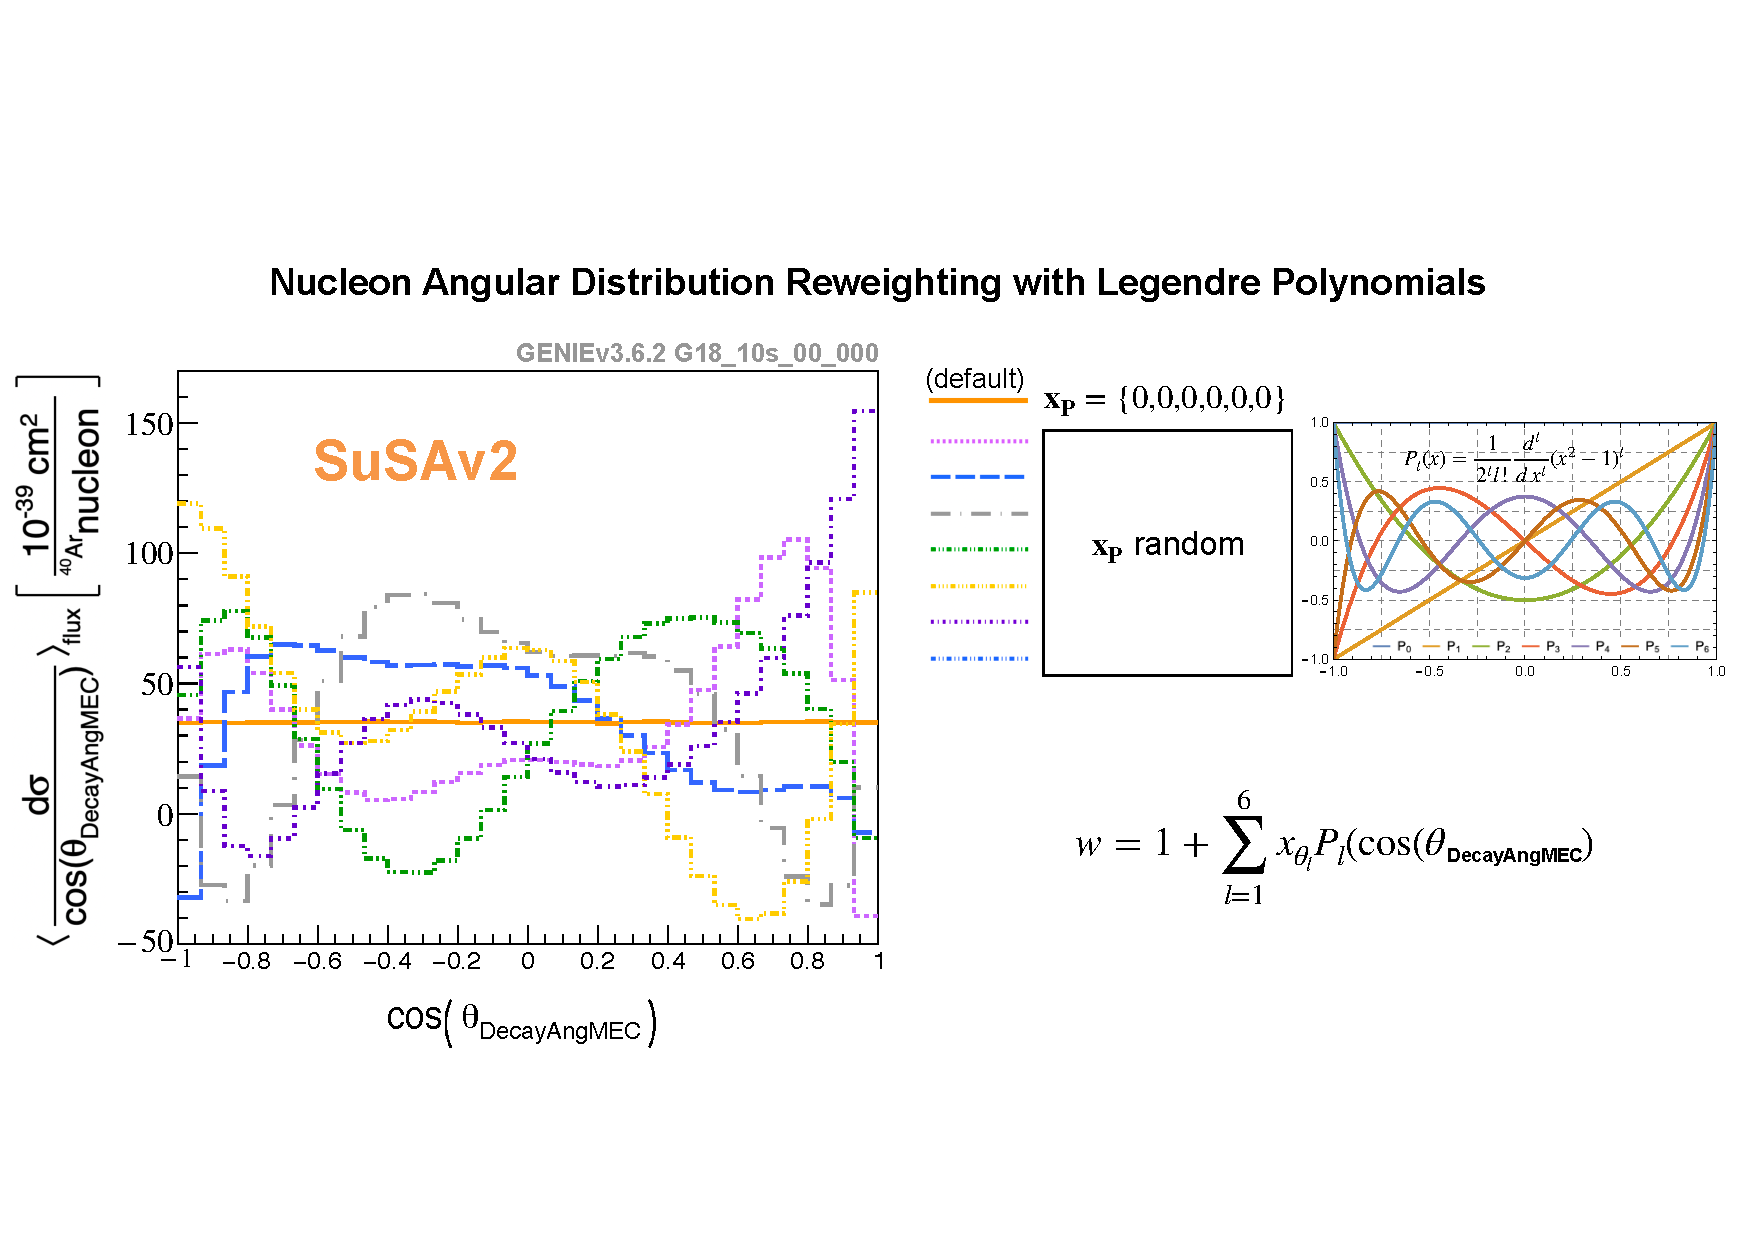
\includegraphics[width=\textwidth]{figures/DecayAngMEC/decayangmec_legendre_susav2.pdf}
    \caption[Nucleon Angular Distribution with Legendre-polynomial Reweighting]{Nucleon Angular Distribution with Legendre-polynomial Reweighting.
    Effect of the \texttt{DecayAngMECLegendre\_CCMEC} parameter on the nucleon angular distribution for the SuSAv2 \acrshort{cc} \acrshort{2p2h} model. The angular distribution is modified using Legendre-polynomial shape variations up to sixth order, while preserving the total cross-section normalisation.}
	\label{fig:decayangmec_legendre_susav2}
    \end{figure}
%
    The weight computation to generate the reweighted $\cos(\theta_\text{DecayAngMEC})$ distrbutions in \Cref{fig:decayangmec_legendre_susav2} is obtained using randomly generated values of the tweak dial values shown in \Cref{fig:decayangmeclegendre_twkDials} 
%
    \begin{figure}[htb]
	\centering
	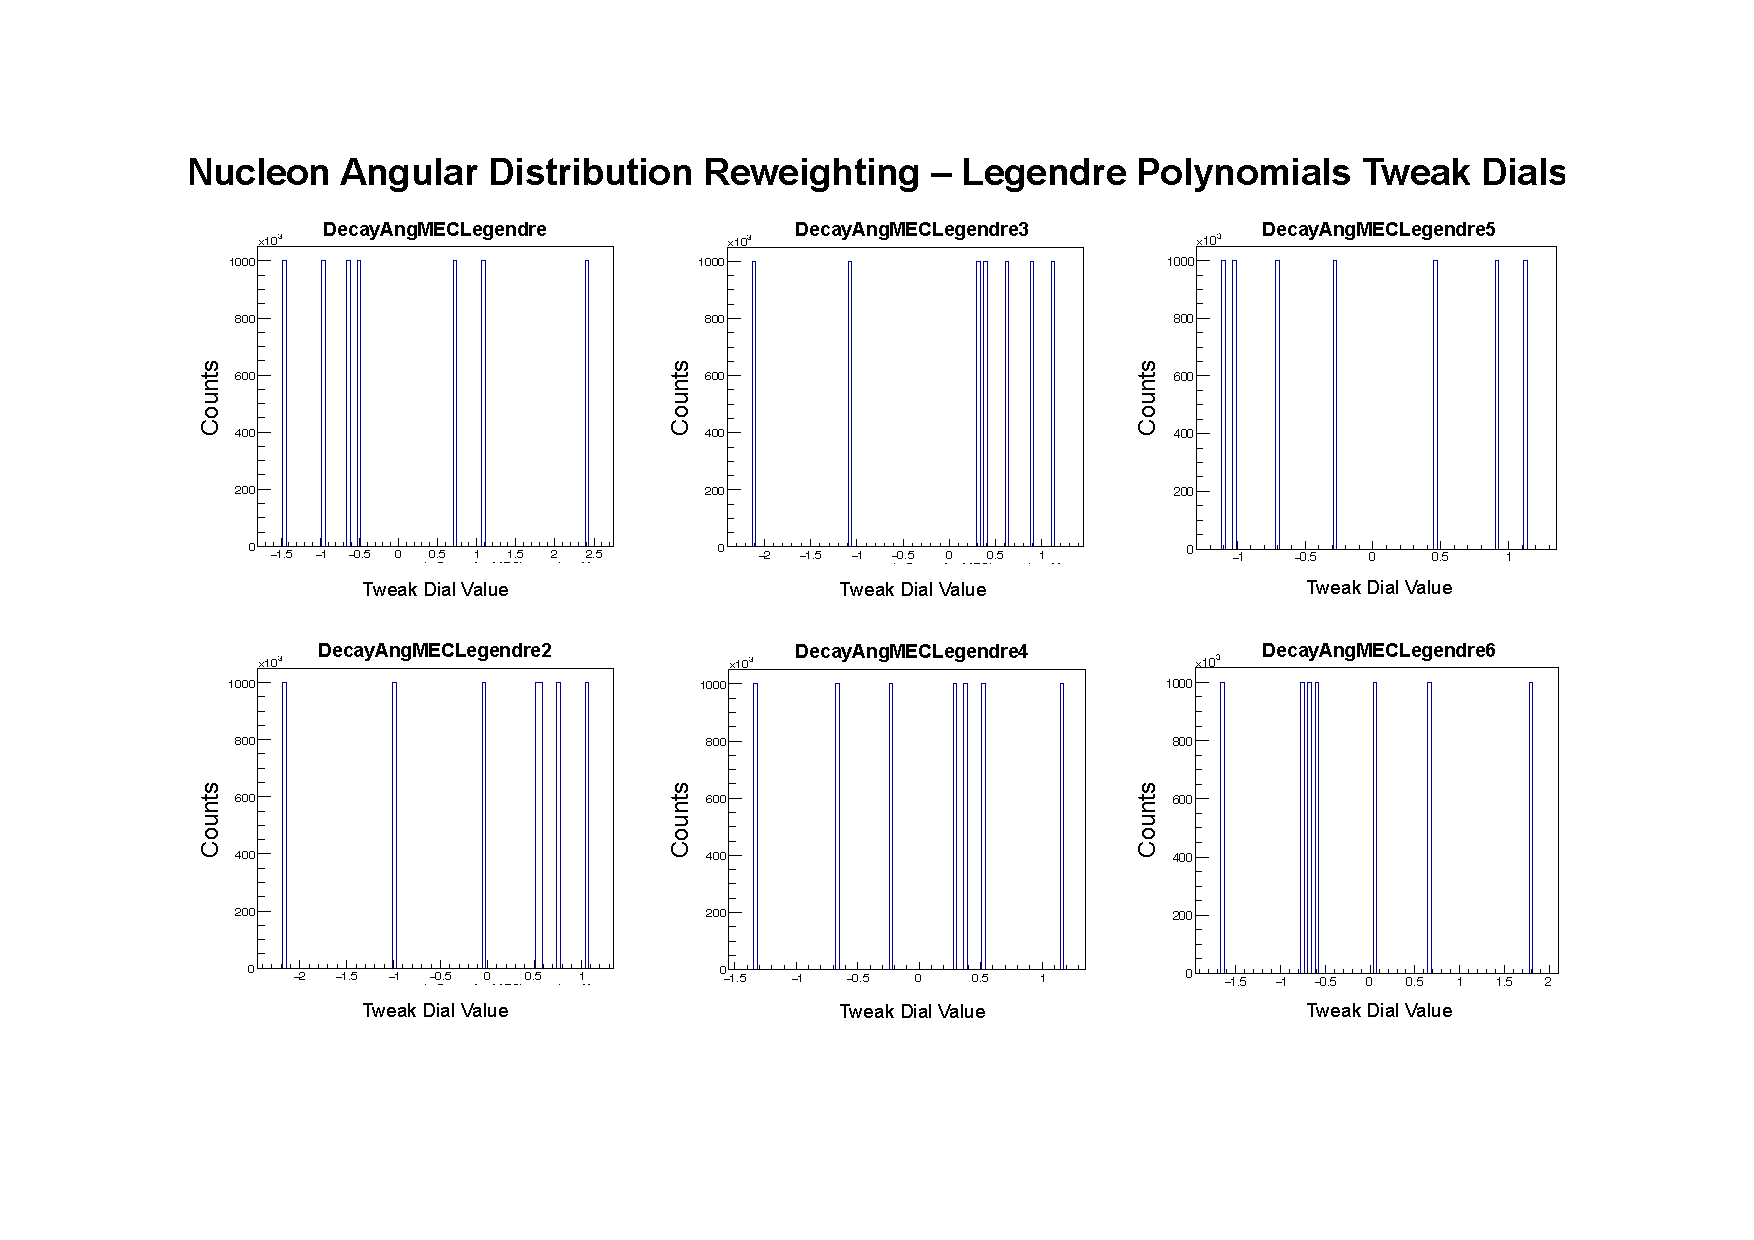
\includegraphics[width=\textwidth]{figures/DecayAngMEC/decayangmeclegendre_twkDials.pdf}
    \caption[Nucleon Angular Distribution with Legendre-polynomial Reweighting]{Nucleon Angular Distribution with Legendre-polynomial Reweighting.
    Effect of the \texttt{DecayAngMECLegendre\_CCMEC} parameter on the nucleon angular distribution for the Valencia (left) and Martini et al. (right) \acrshort{cc} \acrshort{2p2h} model. The angular distribution is modified using Legendre-polynomial shape variations up to sixth order, while preserving the total cross-section normalisation.}
	\label{fig:decayangmeclegendre_twkDials}
    \end{figure}
%
The global average of the event weight remains unity both for individual Legendre-mode weights and for their linear combination, since each mode has vanishing average over an isotropic distribution, as shown in \Cref{fig:decayangmeclegendre_weights}.
%
    \begin{figure}[htb]
	\centering
	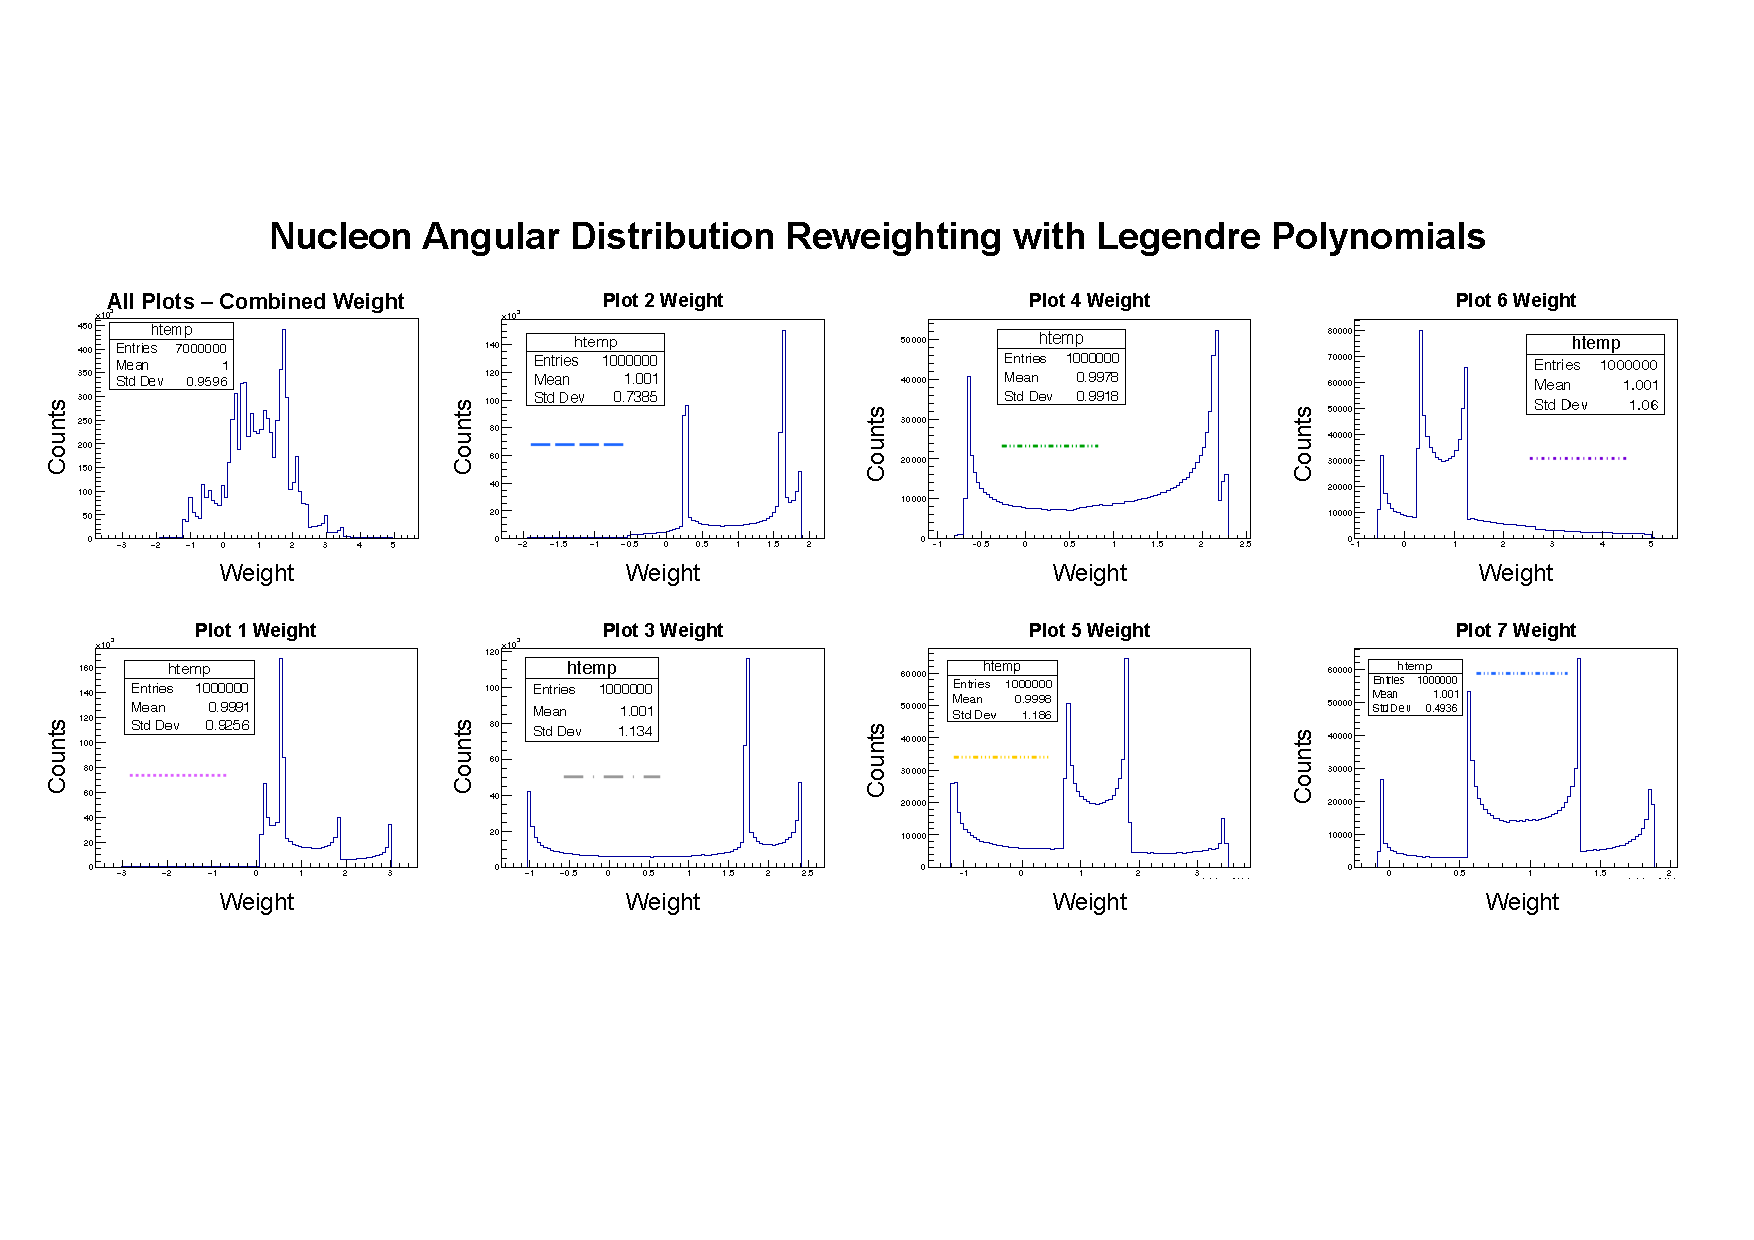
\includegraphics[width=\textwidth]{figures/DecayAngMEC/decayangmeclegendre_weights.pdf}
	\caption[Nucleon Angular Distribution with Legendre Polynomials Parameter]{Nucleon Angular Distribution with Legendre Polynomials Parameter.}
	\label{fig:decayangmeclegendre_weights}
    \end{figure}
%
%
    \begin{figure}[htb]
	\centering
	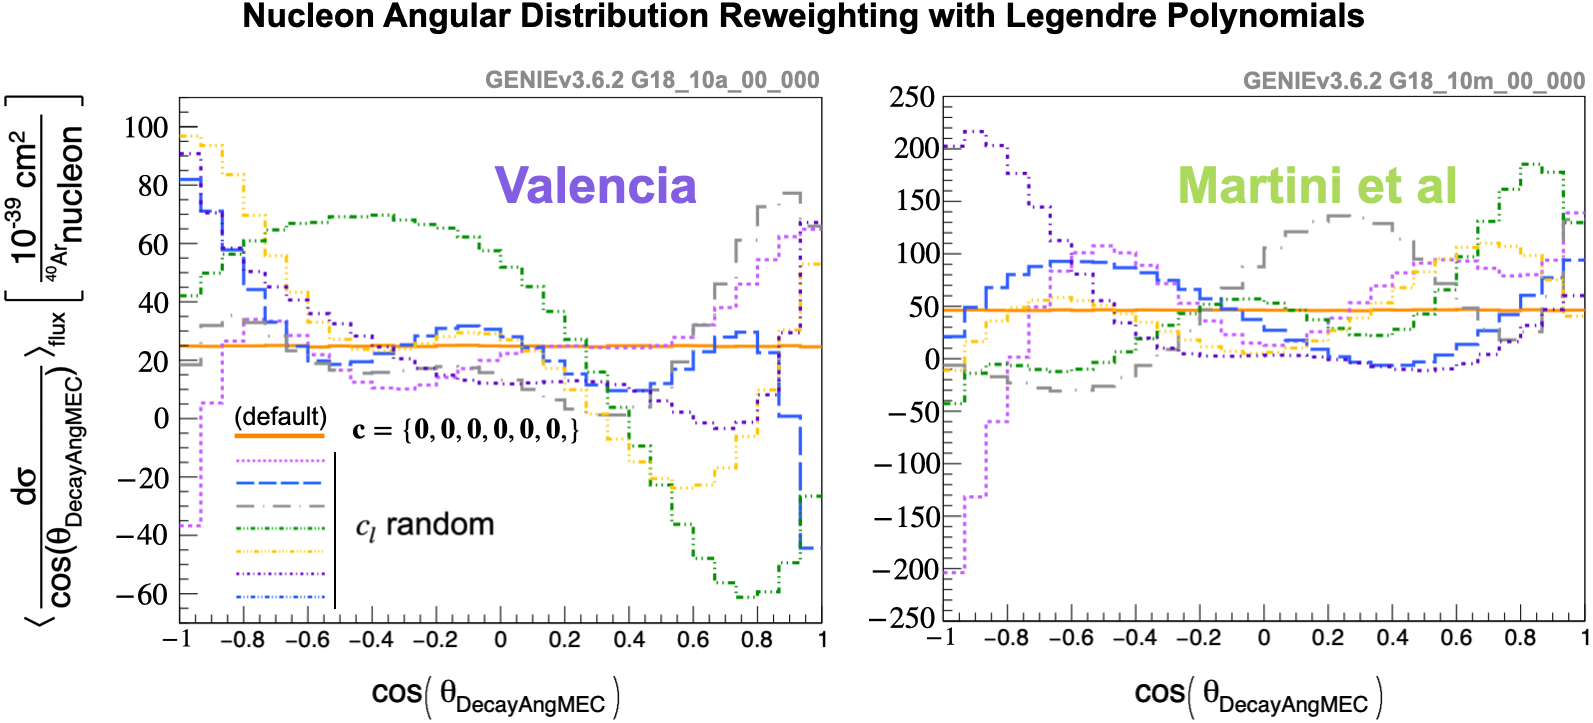
\includegraphics[width=\textwidth]{figures/DecayAngMEC/decayangmec_legendre_valencia_martini.png}
    \caption[Nucleon Angular Distribution with Legendre-polynomial Reweighting]{Nucleon Angular Distribution with Legendre-polynomial Reweighting.
    Effect of the \texttt{DecayAngMECLegendre\_CCMEC} parameter on the nucleon angular distribution for the Valencia (left) and Martini et al. (right) \acrshort{cc} \acrshort{2p2h} model. The angular distribution is modified using Legendre-polynomial shape variations up to sixth order, while preserving the total cross-section normalisation.}
    \label{fig:decayangmec_legendre_valencia_martini}
    \end{figure}
%

\subsection{Nucleon Pair Content} \label{sec:fracpnccmec}
%
A \acrshort{cc} \acrshort{2p2h} interaction occurs on an initial pair of nucleons that either share the same third component of isospin (a nn-bound state of two neutrons for neutrinos and a pp-pair for antineutrinos) or different isospin (a pn-bound state of one neutron and one proton). The $\verb!FracPN_CCMEC!$ parameter adopts a fractional uncertainty of $\pm20\%$ by adjusting the fraction of events involving an initial pn pair relative to the default prediction of the input \acrshort{cc} \acrshort{2p2h} model 
\cite{PhysRevD.105.072001}. The probability for observing a given set of lepton ($l$) kinetic energy $T_l$ and cosine of the scattering angle $\cos(\theta_l)$ for a $\nu$-np scattering event is proportional to the partial differential cross section
%
\begin{align} \label{eq:FracPN_CCMEC_diff_xsec_np}
    P\left( T_l, \cos(\theta_l)|\text{np} \right) 
    \propto
    \dfrac{\mathrm{d}\sigma_{\text{np}}}{\mathrm{d}T_l\cos(\theta_l)}\  \text{,}
\end{align}
%
while the probability for observing the same lepton kinematics given any initial nucleon bound pair is proportional to the total differential cross section
%
\begin{align} \label{eq:FracPN_CCMEC_diff_xsec_tot}
    P\left( T_l, \cos(\theta_l)|\text{all nucleon bound states} \right) 
    \propto
    \dfrac{\mathrm{d}\sigma_{\text{tot}}}{\mathrm{d}T_l\cos(\theta_l)} \ \text{.}
\end{align}
%
Normalising the partial contribution (\Cref{eq:FracPN_CCMEC_diff_xsec_np}) to the total cross section (\Cref{eq:FracPN_CCMEC_diff_xsec_tot}) yields the probability that a given event originates from an initial np pair at fixed kinematics ($T_l, \cos(\theta_l)$):
%
\begin{align} \label{eq:FracPN_CCMEC_xsec_ratio}
    P\left( \text{np} | T_l, \cos(\theta_l) \right) = \dfrac{\mathrm{d}\sigma_\text{np}}{\mathrm{d}T_l\cos(\theta_l)} \Bigg/ \dfrac{\mathrm{d}\sigma_\text{tot}}{\mathrm{d}T_l\cos(\theta_l)}
\end{align}
%
The event weight is constructed as the likelihood ratio between the modified and nominal probabilities for the interaction to occur on an initial np pair. The modified default model's probability is obtained by applying the tweak dial $x_\text{np}$ in combination with an assigned fractional uncertainty $\delta_\text{np}$ to the nominal default model's prediction\footnote{The likelihood ratio in the final event weight $w^\text{FracPN\_CCMEC}$ in \Cref{eq:FracPN_CCMEC_weight} simplifies to a constant scaling factor, as the np fraction cancels explicitly between numerator and denominator.}. The resulting weight associated with the $\verb!FracPN_CCMEC!$ parameter is: 
%
\begin{align} \label{eq:FracPN_CCMEC_weight}
w^\text{FracPN\_CCMEC}
=
\begin{cases}
\left( 1 + x_{\text{np}} \cdot \delta_{\text{np}} \right)
&
\text{np event}
\\[2ex]
\dfrac{
1 -
\left(\dfrac{\mathrm{d}\sigma_{\text{np}}}{\mathrm{d}T_l\cos(\theta_l)} \middle/ \dfrac{\mathrm{d}\sigma_{\text{tot}}}{\mathrm{d}T_l\cos(\theta_l)}\right)
\left( 1 + x_{\text{np}} \cdot \delta_{\text{np}} \right)
}{
1 -
\left(\dfrac{\mathrm{d}\sigma_{\text{np}}}{\mathrm{d}T_l\cos(\theta_l)} \middle/ \dfrac{\mathrm{d}\sigma_{\text{tot}}}{\mathrm{d}T_l\cos(\theta_l)}\right)
}
&
\text{non–np event}
\end{cases}
\end{align}
%
Every unit of weight gained by up-normalising the kinematics in pn events is compensated for by a down-scaling of non-pn event distributions.
The effect of the $\verb!FracPN_CCMEC!$ tweak dial variation is shown in \cref{fig:fracpn_nip} for all three input models in the proton multiplicity distribution of the intermediate-nucleons exiting the neutrino interaction vertex. 
%
\iffalse
%
\begin{figure}[htb!]
	\begin{subfigure}[b]{.319\textwidth}
        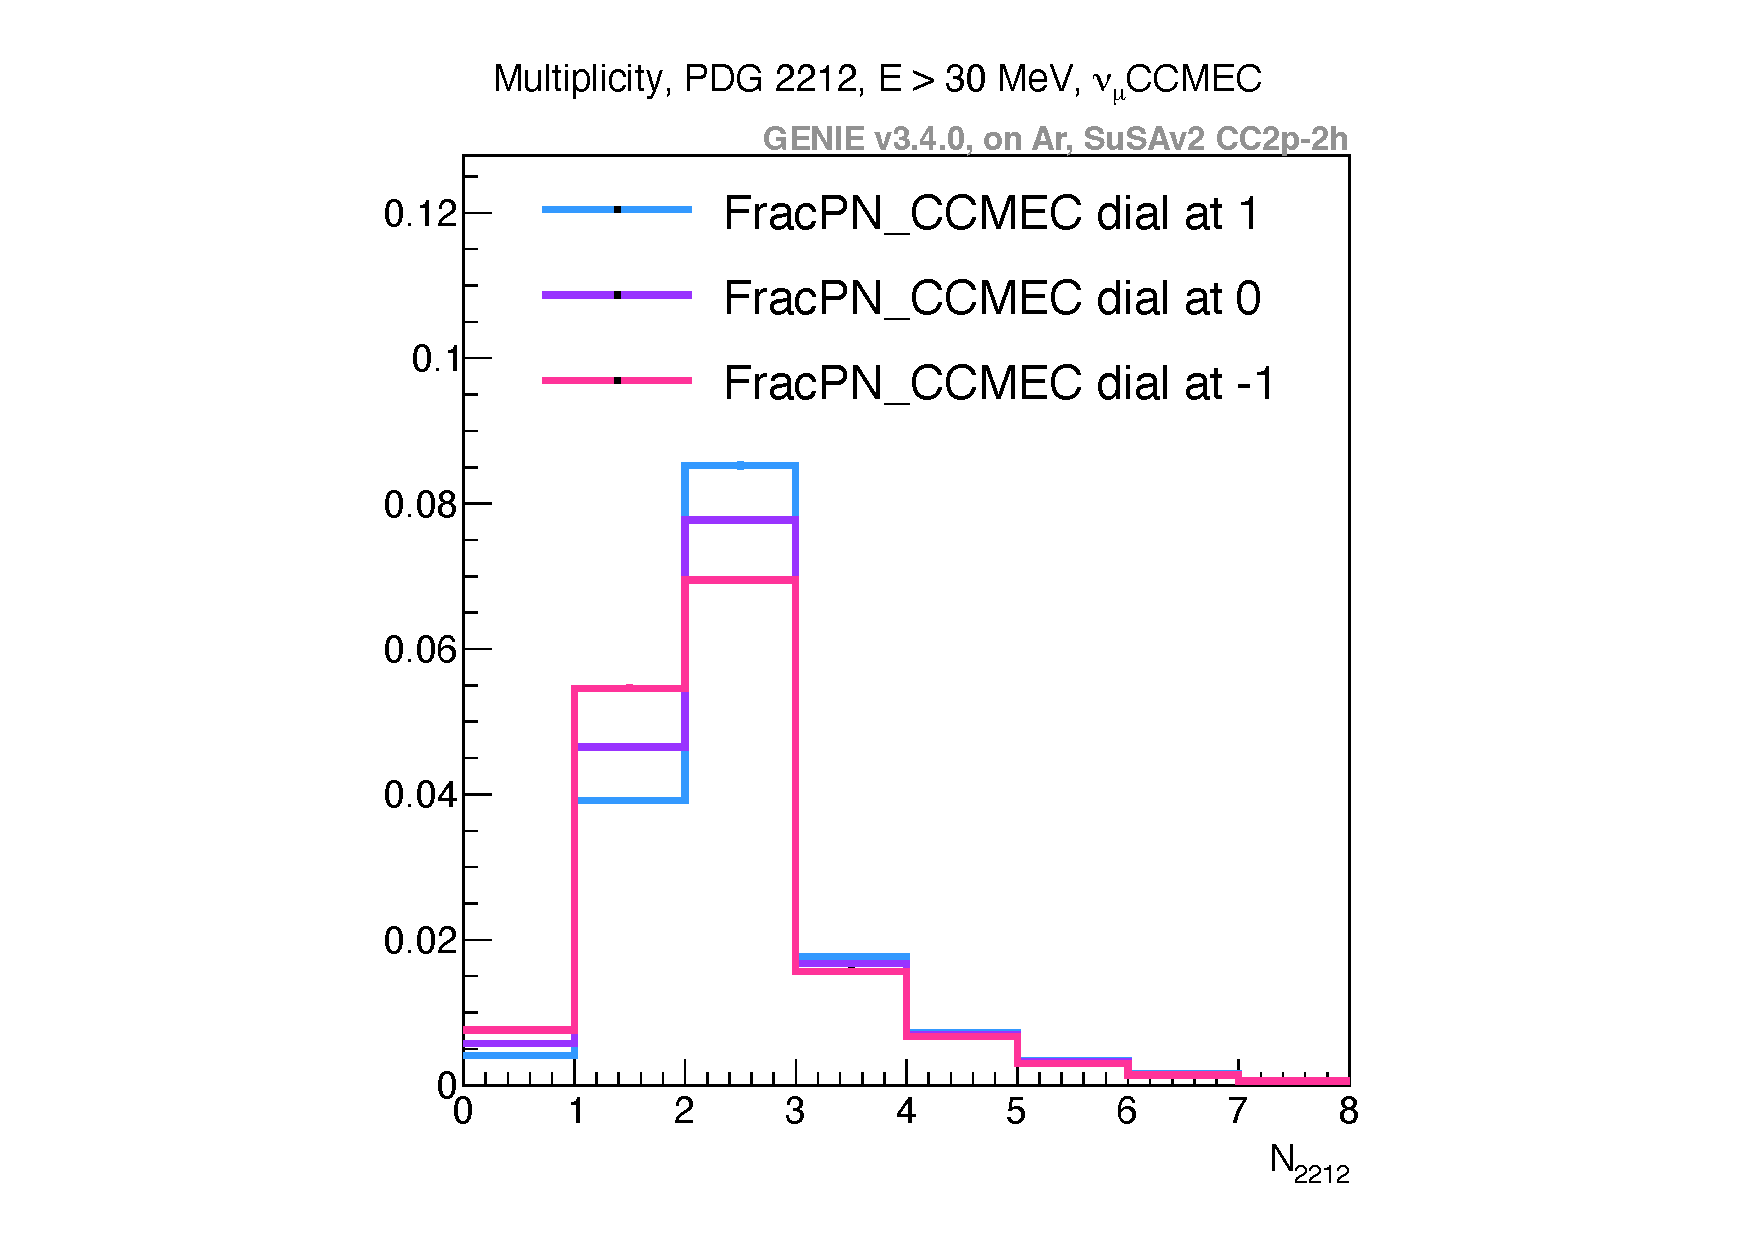
\includegraphics[width=\textwidth]{figures/FracPN_CCMEC/1DComp_mult_2212_14_ccmec_multp_30MeV_edited.pdf}
%	\caption{}
	\label{fracpnccmec_a}
    \end{subfigure}
	\begin{subfigure}[b]{.332\textwidth}
        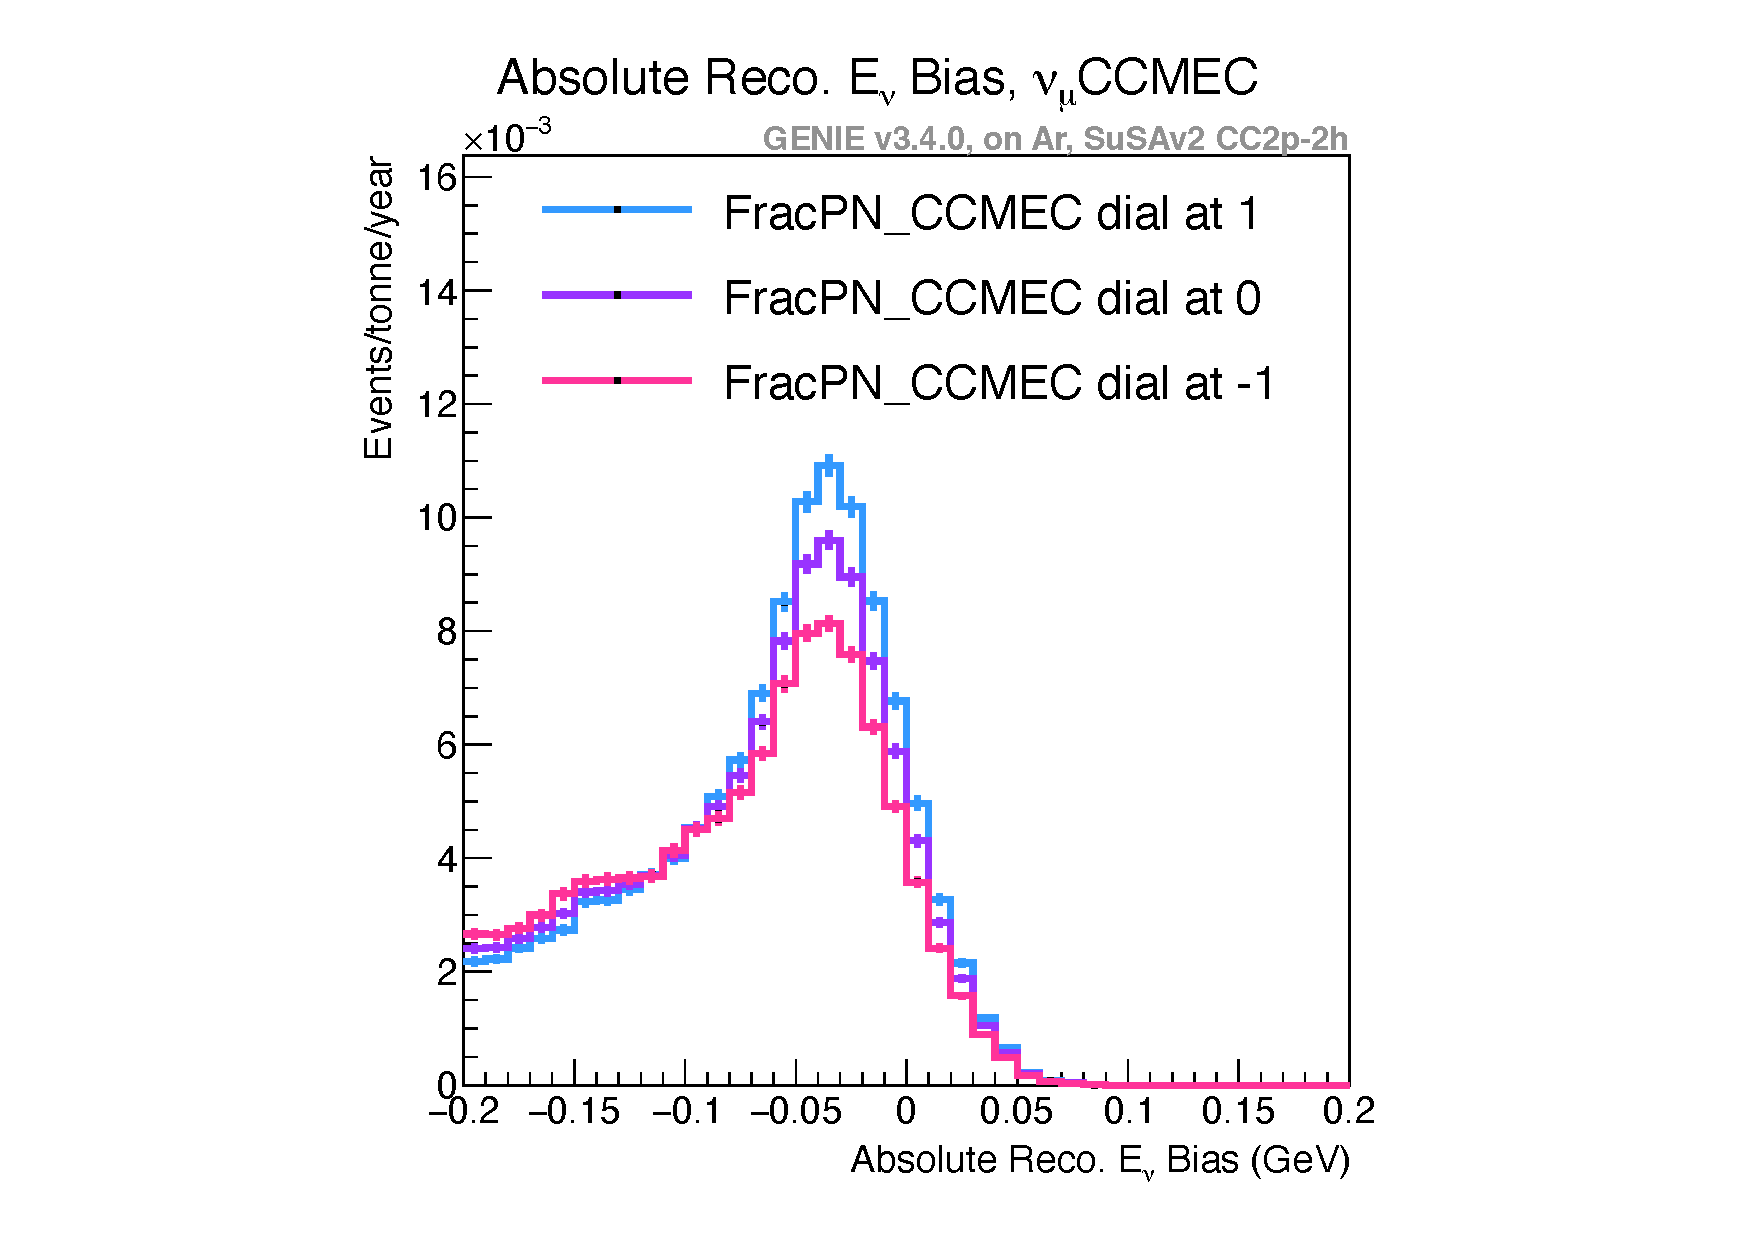
\includegraphics[width=\textwidth]{figures/FracPN_CCMEC/1DComp_ErecAbsBias_14_ccmec_edited.pdf}
	\label{fracpnccmec_b}
    \end{subfigure}
	\begin{subfigure}[b]{.328\textwidth}
        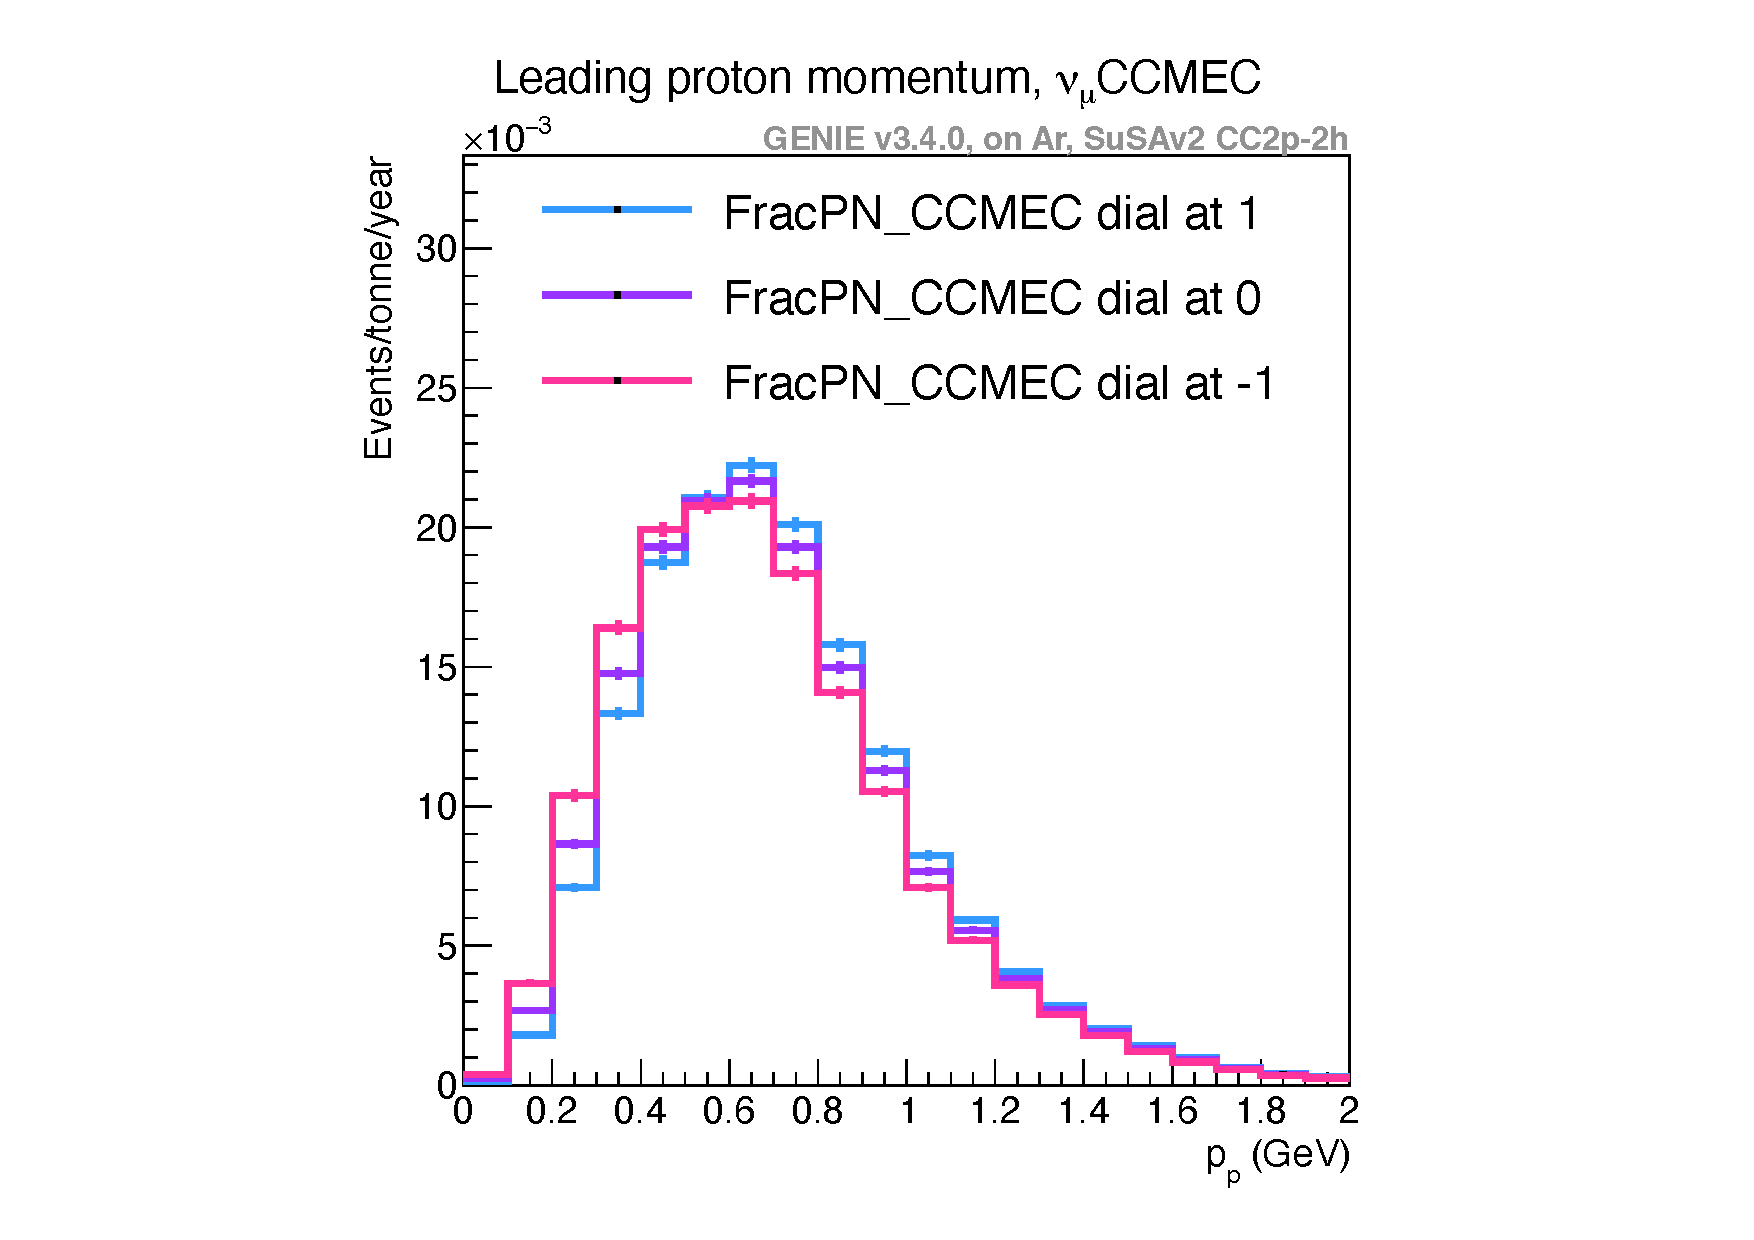
\includegraphics[width=\textwidth]{figures/FracPN_CCMEC/1DComp_LeadP_p_14_ccmec_edited.pdf}
%	\caption{}
	\label{fracpnccmec_c}
    \end{subfigure}
    \vspace{-6mm}
	\caption[]{FracPN\_CCMEC dials for proton multiplicity, energy bias and $p_p$ (from left to right).}
	\label{fracpnccmec_plots}
\end{figure}
%
\fi
%
    \begin{figure}[H]
	\centering
	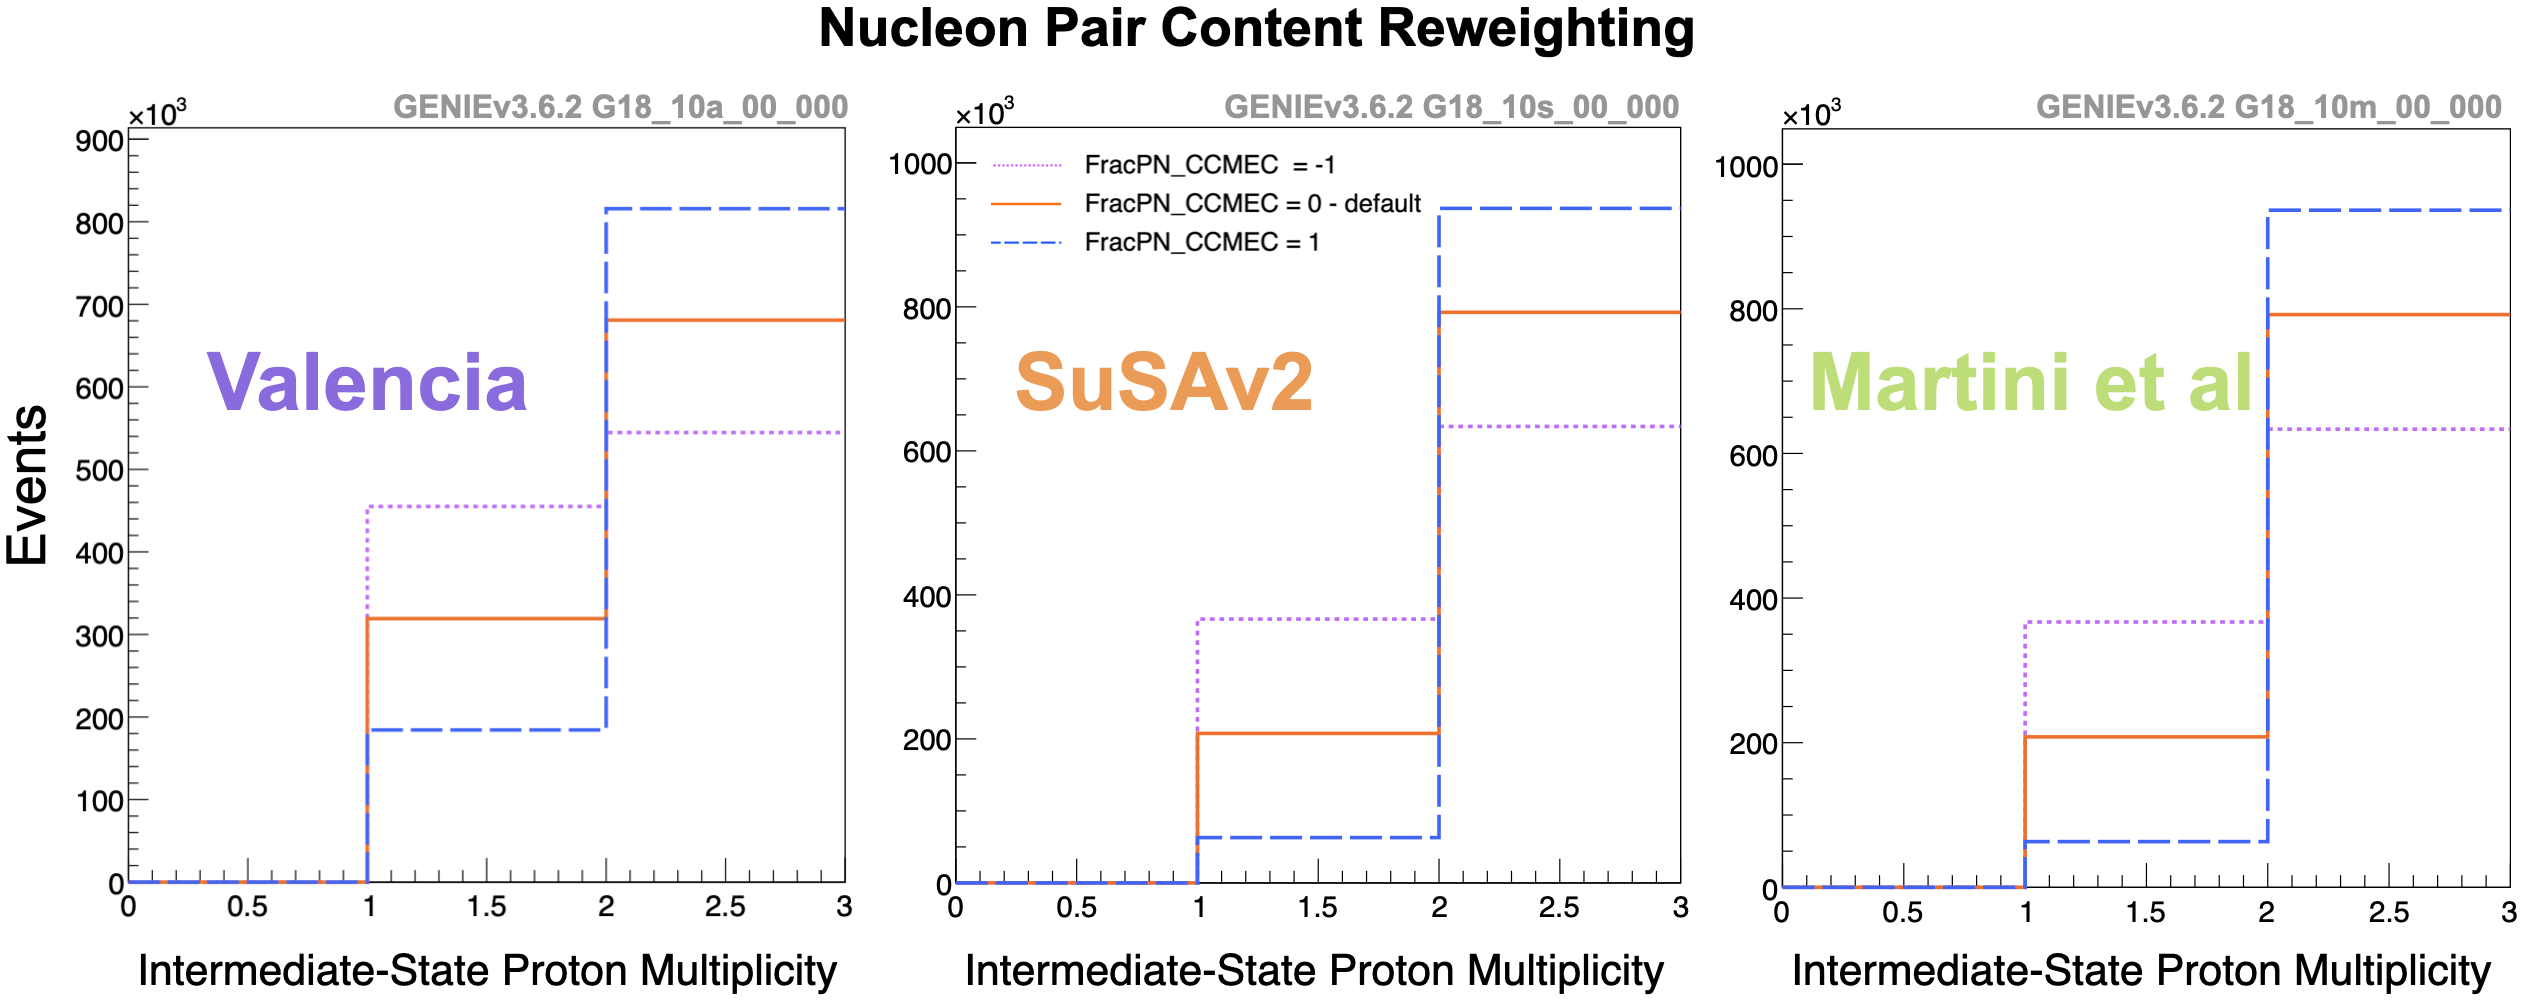
\includegraphics[width=\textwidth]{figures/FracPN_CCMEC/fracpn_nip.png}%{figures/FracPN_CCMEC/fracpn_nip.pdf}
	\caption[Nucleon Pair Content Parameter]{Nucleon Pair Content Parameter. The \texttt{FracPN\_CCMEC} modifies the fraction of neutrino interactions on np pairs and thereby alters the resulting intermediate-state multiplicity. Increasing the np-pair fraction leads to an increase in the number of $2$-proton intermediate states. Conversely, more an increased np-pair fraction means a reduced nn-pair fraction, resulting in less $1$-p intermediate states. The effect of varying the \texttt{FracPN\_CCMEC} tweak dials on the intermediate-state proton muliplicity is consistent across the \acrshort{2p2h} Valencia, SuSAv2 and Martini et al. models.}
	\label{fig:fracpn_nip}
    \end{figure}
%
Varying the $\verb!FracPN_CCMEC!$ tweak dial modifies the fraction of $\nu$-np interactions relative to $\nu$-nn interactions. Positive (negative) dial values increase (decrease) the fraction of $\nu$-np pair scattering. As a result, the relative abundance of $2$-proton intermediate states increases (decreases), while the fraction of $1$-proton intermediate states is correspondingly reduced. Hence, deviations from the $\verb!FracPN_CCMEC!$ tweak dial central value at $0$ lead to systematic changes in the proton multiplicity of the event's intermediate-state topology.
The effect on the proton multiplicity in the final state is shown in \Cref{fig:fracpn_nfp}.
%
    \begin{figure}[H]
	\centering
	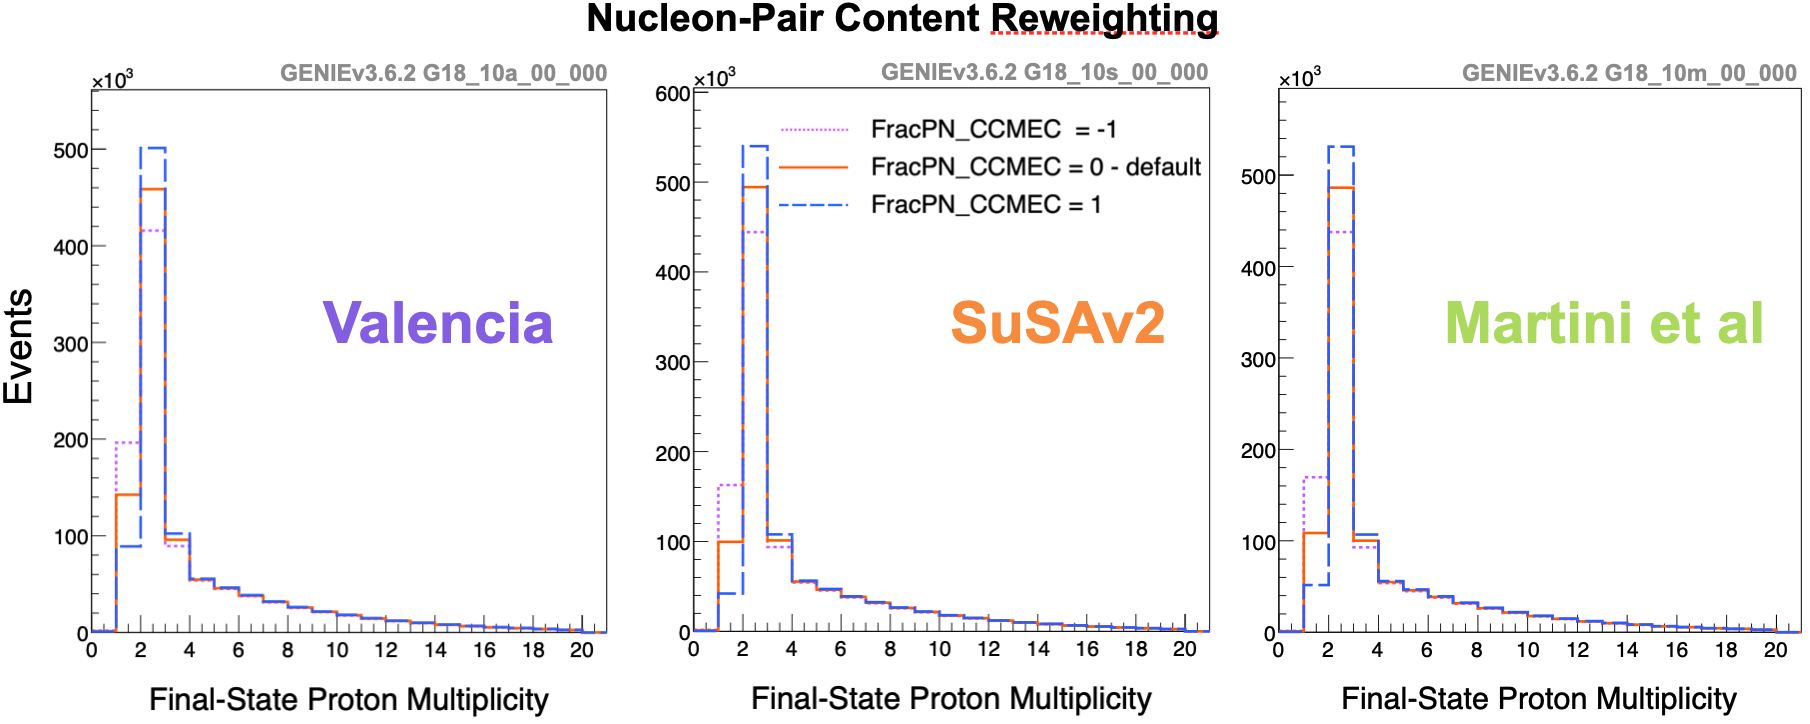
\includegraphics[width=\textwidth]{figures/FracPN_CCMEC/fracpn_nfp.png}
	\caption[Proton Multiplicity in the Final State]{Proton multiplicity in the final state for variations of the \texttt{FracPN\_CCMEC} parameter.}
	\label{fig:fracpn_nfp}
    \end{figure}
%
In contrast to the intermediate-state multiplicity, \acrshort{fsi}s obscure the relationship between the initial-state nucleon-pair configuration and the observed final-state proton multiplicity. However, although \acrshort{fsi}s modify the final-state topology, the proton multiplicity is consistent with the observed intermediate-state proton multiplicity shown in \Cref{fig:fracpn_nip}.

\subsection{Cross-Section Model-Shape Differences} \label{sec:xsecshapeccmec}
%\paragraph{Cross-Section Variations}
When propagating neutrino-nucleus cross-section uncertainties, the neutrino interaction rate is modified directly through event reweighting. This approach avoids regenerating events and is therefore largely independent of the generator implementation, but it still relies on the underlying physics model used to produce the events. Event reweighting is performed by computing the ratio of the differential
cross section evaluated with modified physics parameters $P'$ to that
obtained with the nominal parameters $P$ at a given point in $n$-dimensional phase
space $K^n$ \cite{Andreopoulos:2009rq}:
%
\begin{align} \label{event_weight}
    w_\sigma = \frac{\text{d}^n\sigma'(K,P')}{\text{d}K^n} \bigg/ \frac{\text{d}^n\sigma(K,P)}{\text{d}K^n}
\end{align}
%
In order to account for differences in theoretical predictions of lepton kinematics on \acrshort{cc} \acrshort{2p2h} scattering, the $\verb!XSecShape_CCMEC!$ parameter modifies the shape of the inclusive differential cross section by interpolating between a default calculation and an alternative prediction:
%
\begin{align} \label{weight_XSecShape_CCMEC}
    w^\text{XSecShape\_CCMEC} = \dfrac{(1-x_X) \cdot \dfrac{\mathrm{d}^2\sigma^{def}}{\mathrm{d}T_\ell \mathrm{d}\cos(\theta_\ell)} + x_X \cdot \dfrac{\mathrm{d}^2\sigma^{alt}}{\mathrm{d}T_\ell \mathrm{d}\cos(\theta_\ell)}}{\dfrac{\mathrm{d}^2\sigma^{def}}{\mathrm{d}T_\ell \mathrm{d}\cos(\theta_\ell)}}
\end{align}
%
Varying the tweak dial $x_X$ associated with the $\verb!XSecShape_CCMEC!$ parameter continuously on an interval $[0,1]$ allows a linear interpolation between a default and alternative model. Since the interpolation is performed relative to the default cross section, the normalisation of the reweighted cross section remains unchanged with respect to the nominal prediction. \acrshort{2p2h} model shape differences are usually considered in the three-momentum transfer $|\vec{q}|$ versus energy transfer $\omega$ phase space. The predictions for the $\omega$ vs. $|\vec{q}|$ distributions by the Empirical, Valencia, SuSAv2 and Martini et al. \acrshort{genie}-models are shown in \Cref{fig:genie_2p2h_models_no_stats}.
%
    \begin{figure}[H]
	\centering
	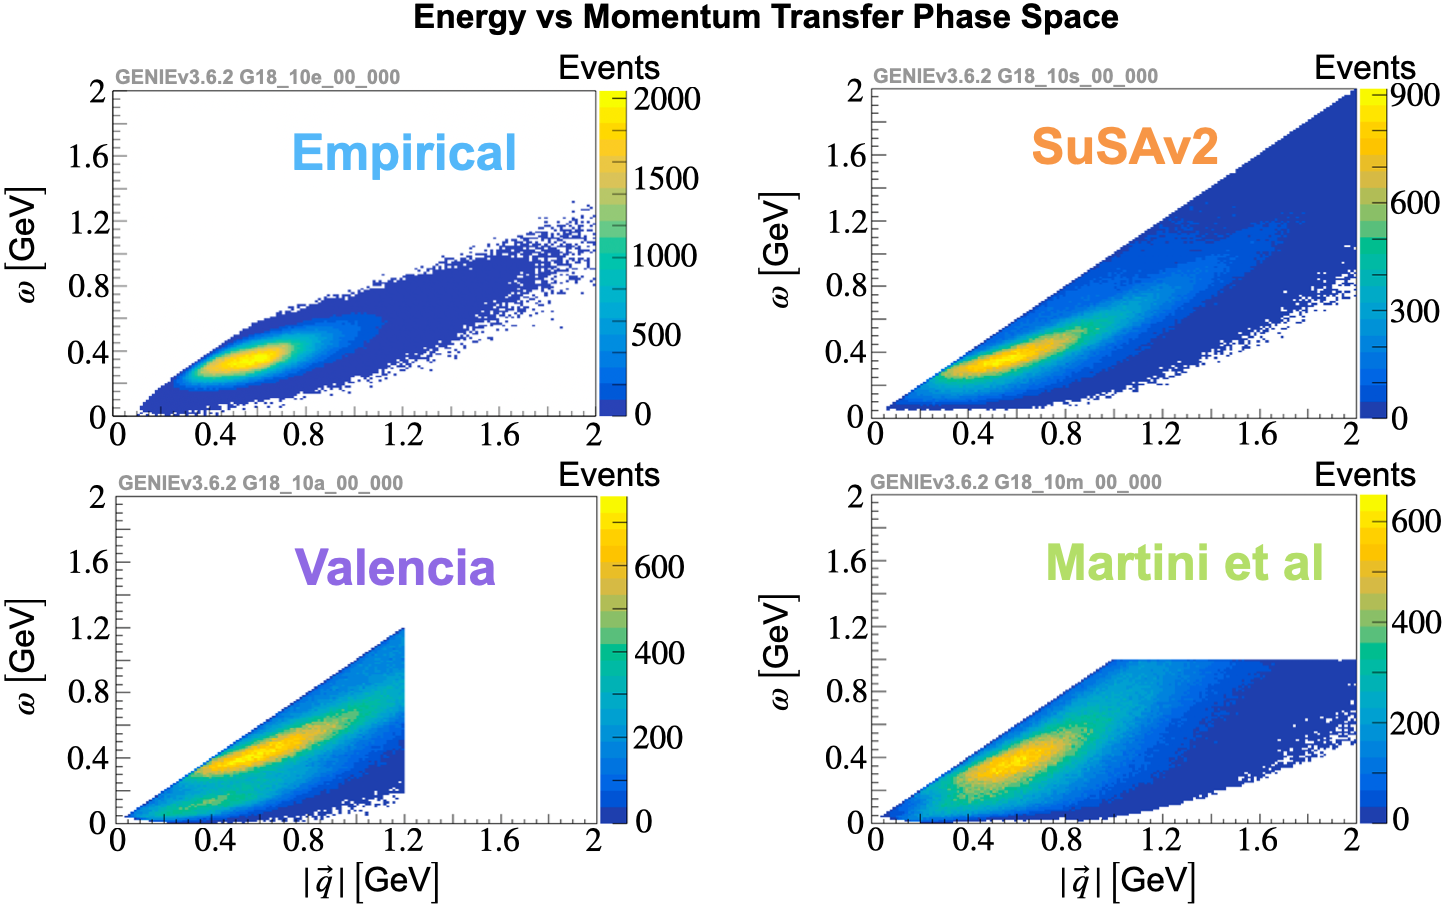
\includegraphics[width=\textwidth]{figures/XSecShape_CCMEC/genie_2p2h_models_no_stats.png}
	\caption[\acrshort{genie} \acrshort{2p2h} Models]{\acrshort{genie} \acrshort{2p2h} Models in the energy- vs 3-momentum-transfer phase space. The shown distributions have been obtained by simulating one million neutrino interactions on argon with the \acrshort{dune} flux.}
	\label{fig:genie_2p2h_models_no_stats}
    \end{figure}
%
Several characteristic features can be identified in the energy-momentum
phase space shown in \Cref{fig:genie_2p2h_models_no_stats}.
The \acrshort{genie} \acrshort{2p2h} Empirical model \cite{Katori:2013eoa} exhibits a sharp single peak.
The \acrshort{genie} \acrshort{2p2h} Valencia model \cite{PhysRevD.88.113007} is limited to $3$-momentum transfer $|\vec{q}|<\SI{1.2}{\GeV}$. The two peaks correspond to two distinct dynamical mechanisms. The peak at higher energy transfer corresponds to the $\Delta\Delta$-resonance contribution and the lower-energy transfer peak is associated with the N$\Delta$-resonance component. Their relative separation corresponds to the mass difference between a nucleon N and a delta $\Delta$, which is around $\SI{0.3}{\GeV}$ \cite{Sobczyk:2020dkn}.
The \acrshort{genie} \acrshort{2p2h} SuSAv$2$ model \cite{Dolan:2019bxf} kinematic distribution with a single peak appears similar in shape compared to the \acrshort{genie} Empirical model prediction, though exhibits a more profound theoretical description \cite{Amaro:2019zos}. 
The Martini-Ericson-Chanfray-Marteau (in the following referred to as Martini et al) model \cite{Russo:2026} is defined over energy transfers between $\SI{0.005}{\GeV} < \omega < \SI{0.995}{\GeV}$ and $3$-momentum transfers between $\SI{0.001}{\GeV} < |\vec{q}| < \SI{2.0}{\GeV} GeV$. Its distribution features two overlapping peaks in the $\omega$ vs. $|\vec{q}|$ kinematic phase space. 

Currently there are substantial differences between alternative theoretical predictions of lepton kinematics on \acrshort{cc} \acrshort{2p2h} scattering in dependence on the chosen model. In order to investigate the currently unknown \acrshort{cc} \acrshort{2p2h} cross-section shape, the $\verb!XSecShape_CCMEC!$ parameter modifies the shape of the inclusive \acrshort{cc} \acrshort{2p2h} differential cross section between the GENIE Empirical model \cite{10.1063/1.4919465}, the Valencia model \cite{PhysRevD.88.113007} and the SuSAv$2$ model \cite{Amaro_2020}. By varying the tweak dials associated with the $\verb!XSecShape_CCMEC!$, $\verb!XSecShape_CCMEC_Empirical!$ and $\verb!XSecShape_CCMEC_Martini!$ parameters, a linear interpolation allows for continuous variations of the dial in order to explore the shape of respective distributions and how they change shape when renormalising the distributions from one model shape to another. The input default and target model combinations using the cross-section shape variation parameters developed in this work are summarised in \Cref{tab:xsecshape_summary}.
%
\iffalse
\begin{table}[htb]
\centering
\caption{Summary of \texttt{XSecShape\_CCMEC} reweighting parameters and their effect on the input \acrshort{2p2h} model predictions.}
\begin{tabular}{lcccc}
\toprule
Parameter 
& \textcolor{violet}{Valencia} 
& \textcolor{orange}{SuSAv2} 
& \textcolor{green!60!black}{Martini et al.} 
& Empirical \\
\midrule

\texttt{XSecShape\_CCMEC} 
& $\leftrightarrow$ \textcolor{orange}{SuSAv2} 
& $\leftrightarrow$ \textcolor{violet}{Valencia} 
& $\rightarrow$ \textcolor{orange}{SuSAv2} 
& --- \\

\texttt{XSecShape\_CCMEC\_Empirical} 
& $\rightarrow$ Empirical 
& $\rightarrow$ Empirical 
& $\rightarrow$ Empirical 
& --- \\

\texttt{XSecShape\_CCMEC\_Martini} 
& $\rightarrow$ \textcolor{green!60!black}{Martini et al.} 
& $\rightarrow$ \textcolor{green!60!black}{Martini et al.} 
& $\rightarrow$ \textcolor{violet}{Valencia} 
& --- \\

\bottomrule
\end{tabular}
\label{tab:xsecshape_summary}
\end{table}
\fi
%
\begin{table}[htb]
\centering
\small
\caption{Summary of cross-section shape reweighting parameters \texttt{XSecShape\_CCMEC}, \texttt{XSecShape\_CCMEC\_Empirical} and \texttt{XSecShape\_CCMEC\_Martini}. The row labels (Default) denote the nominal input model, whereas the column labels (Target) indicate the alternative model that the parameters are reweighting to. Entries specify which parameter enables interpolation from the default model (row) to the target model (column). For readability, the suffix '\texttt{\_CCMEC}' has been omitted from the parameter names.}
%
\resizebox{\textwidth}{!}{
\begin{tabular}{|l|c|c|c|c|}
\hline
\diagbox{Default}{Target}
& \textcolor{valencia!90!black}{Valencia}
& \textcolor{susav!90!black}{SuSAv2}
& \textcolor{martini!90!black}{Martini et al.}
& \textcolor{empirical!90!black}{Empirical} \\
\hline

\textcolor{valencia!90!black}{Valencia}
& ---
& \texttt{XSecShape}
& \texttt{XSecShape\_Martini}
& \texttt{XSecShape\_Empirical} \\
\hline

\textcolor{susav!90!black}{SuSAv2}
& \texttt{XSecShape}
& ---
& \texttt{XSecShape\_Martini}
& \texttt{XSecShape\_Empirical} \\
\hline

\textcolor{martini!90!black}{Martini et al.}
& \texttt{XSecShape\_Martini}
& \texttt{XSecShape}
& ---
& \texttt{XSecShape\_Empirical} \\
\hline

\end{tabular}
}
\label{tab:xsecshape_summary}
\end{table}
%
The effect of the \acrshort{cc} \acrshort{2p2h} shape dial variations on the distribution of the leptonic energy and momentum transfer for simulated \acrshort{cc} \acrshort{2p2h} events in \acrshort{dune} is illustrated in Figs. (\ref{fig:xsecshape_valenciaTosusav2})-(\ref{fig:xsecshape_overview}).

Figs. (\ref{fig:xsecshape_valenciaTosusav2}) and (\ref{fig:xsecshape_valenciaToempirical}) show the effect of reweighting the Valencia prediction towards the SuSAv2 and Empirical models, respectively.
The initially well-separated two-peak structure of the Valencia distribution (left panel, $x_X = 0$) is gradually transformed into a single-peaked distribution as the interpolation parameter is increased (middle panel, $x_X = 0.5$), ultimately reproducing the target model prediction (right panel, $x_X = 1$).
%
    \begin{figure}[H]
	\centering
	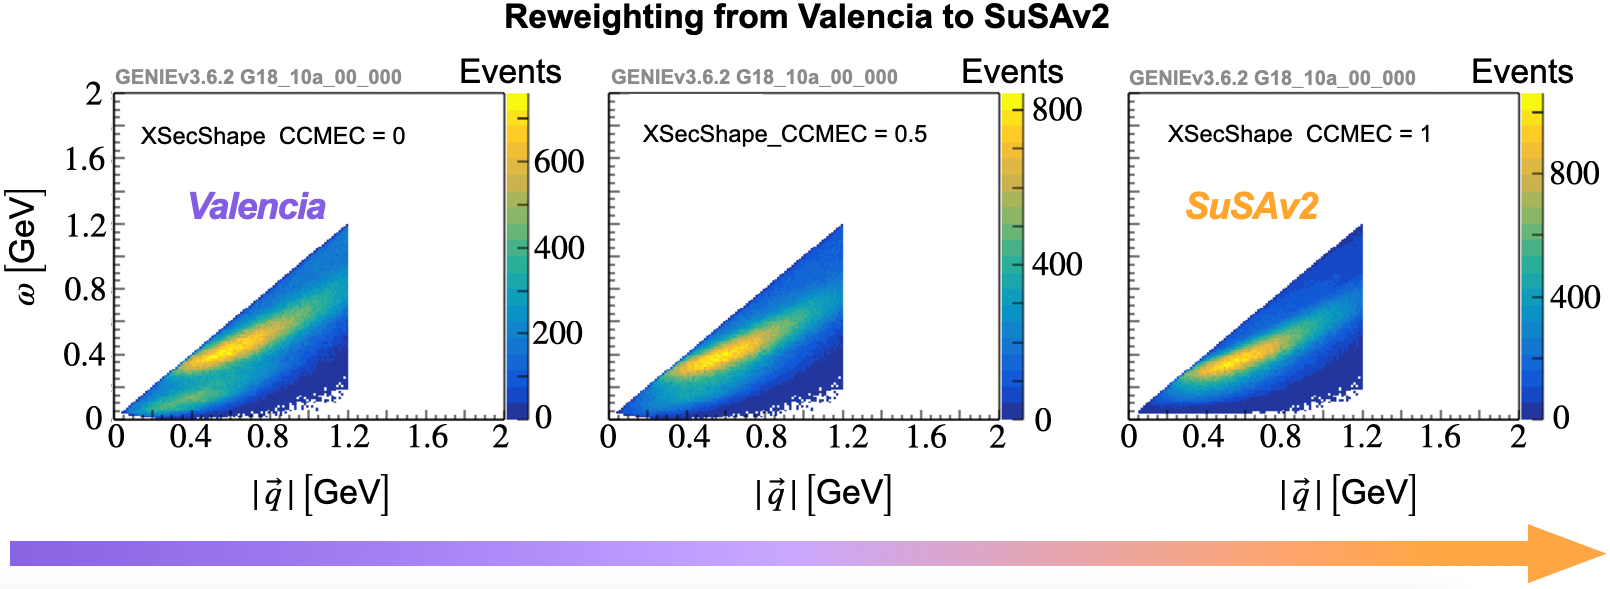
\includegraphics[width=\textwidth]{figures/XSecShape_CCMEC/xsecshape_valenciaTosusav2.png}
	\caption[\texttt{XSecShape\_CCMEC} Parameter: Reweighting from the Valencia to the SuSAv2 Model]{\texttt{XSecShape\_CCMEC} Parameter: Reweighting from the Valencia to the SuSAv2 model.}
	\label{fig:xsecshape_valenciaTosusav2}
    \end{figure}
%

%
    \begin{figure}[H]
	\centering
	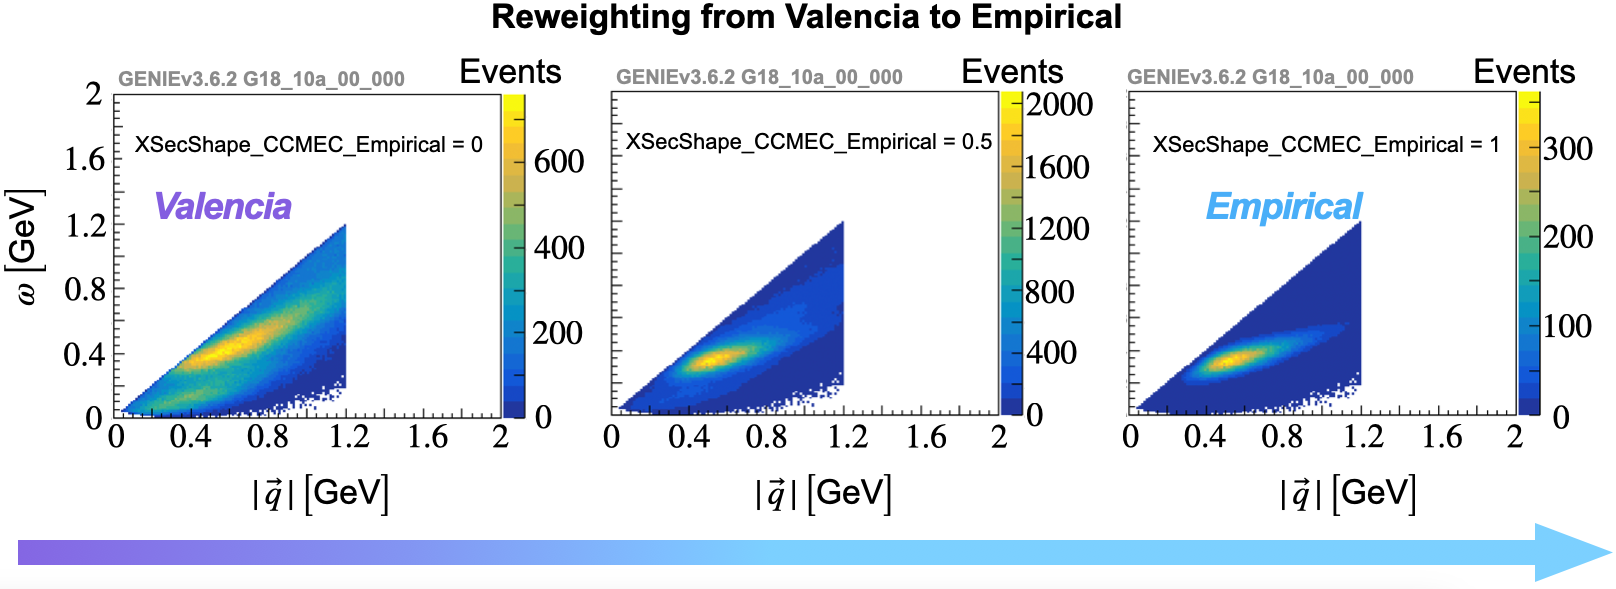
\includegraphics[width=\textwidth]{figures/XSecShape_CCMEC/xsecshape_valenciaToempirial.png}
	\caption[\texttt{XSecShape\_CCMEC\_Empirical} Parameter: Reweighting from the Valencia to the Empirical Model]{\texttt{XSecShape\_CCMEC\_Empirical} Parameter: Reweighting from the Valencia to the Empirical model.}
	\label{fig:xsecshape_valenciaToempirical}
    \end{figure}
%
% 
\iffalse
%
\begin{figure}[htb!]
	\begin{subfigure}[b]{.32\textwidth}
        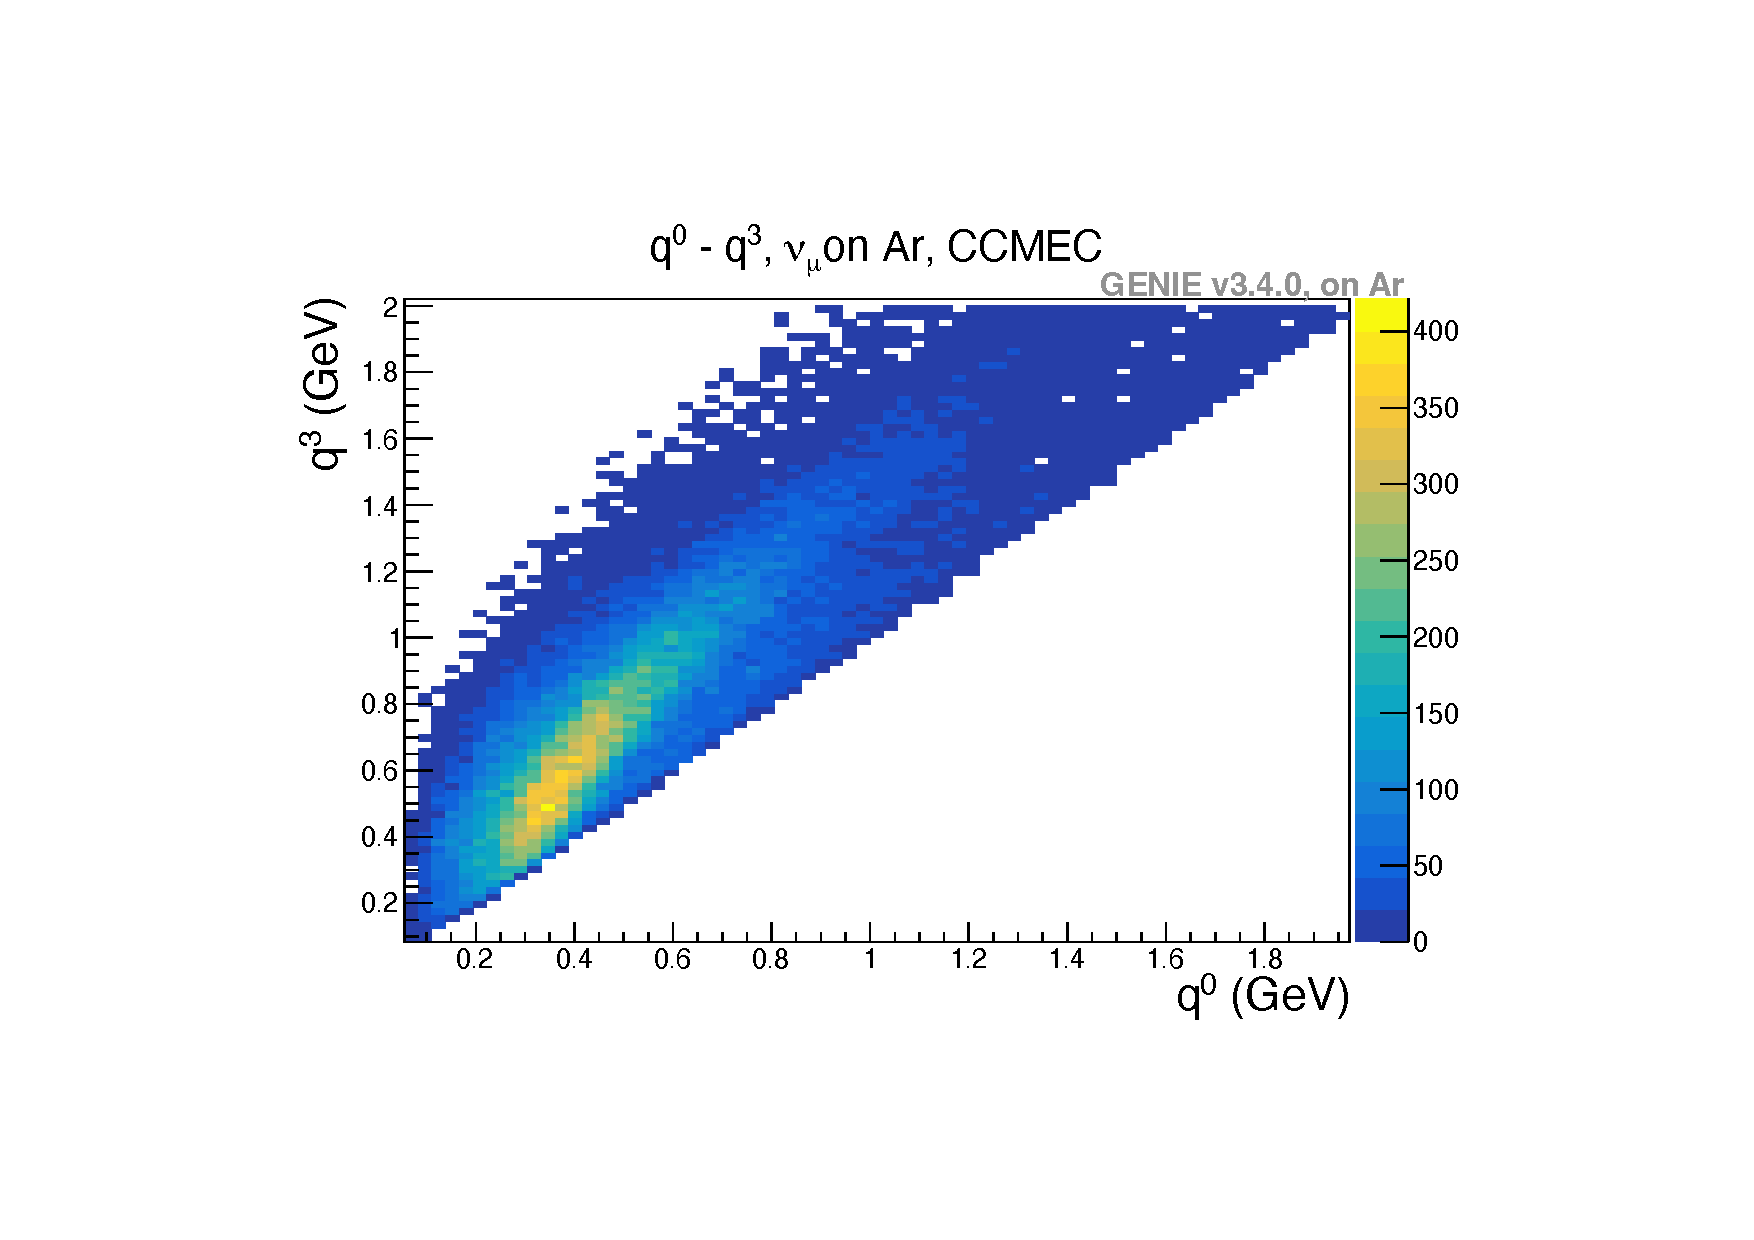
\includegraphics[width=\textwidth]{figures/XSecShape_CCMEC/2DComp_q0-q3_SuSAv2_edited.pdf}
        \vspace{-2.mm}
%	\caption{}
	\label{xsecshapeccmec_a}
    \end{subfigure}
	\begin{subfigure}[b]{.32\textwidth}
        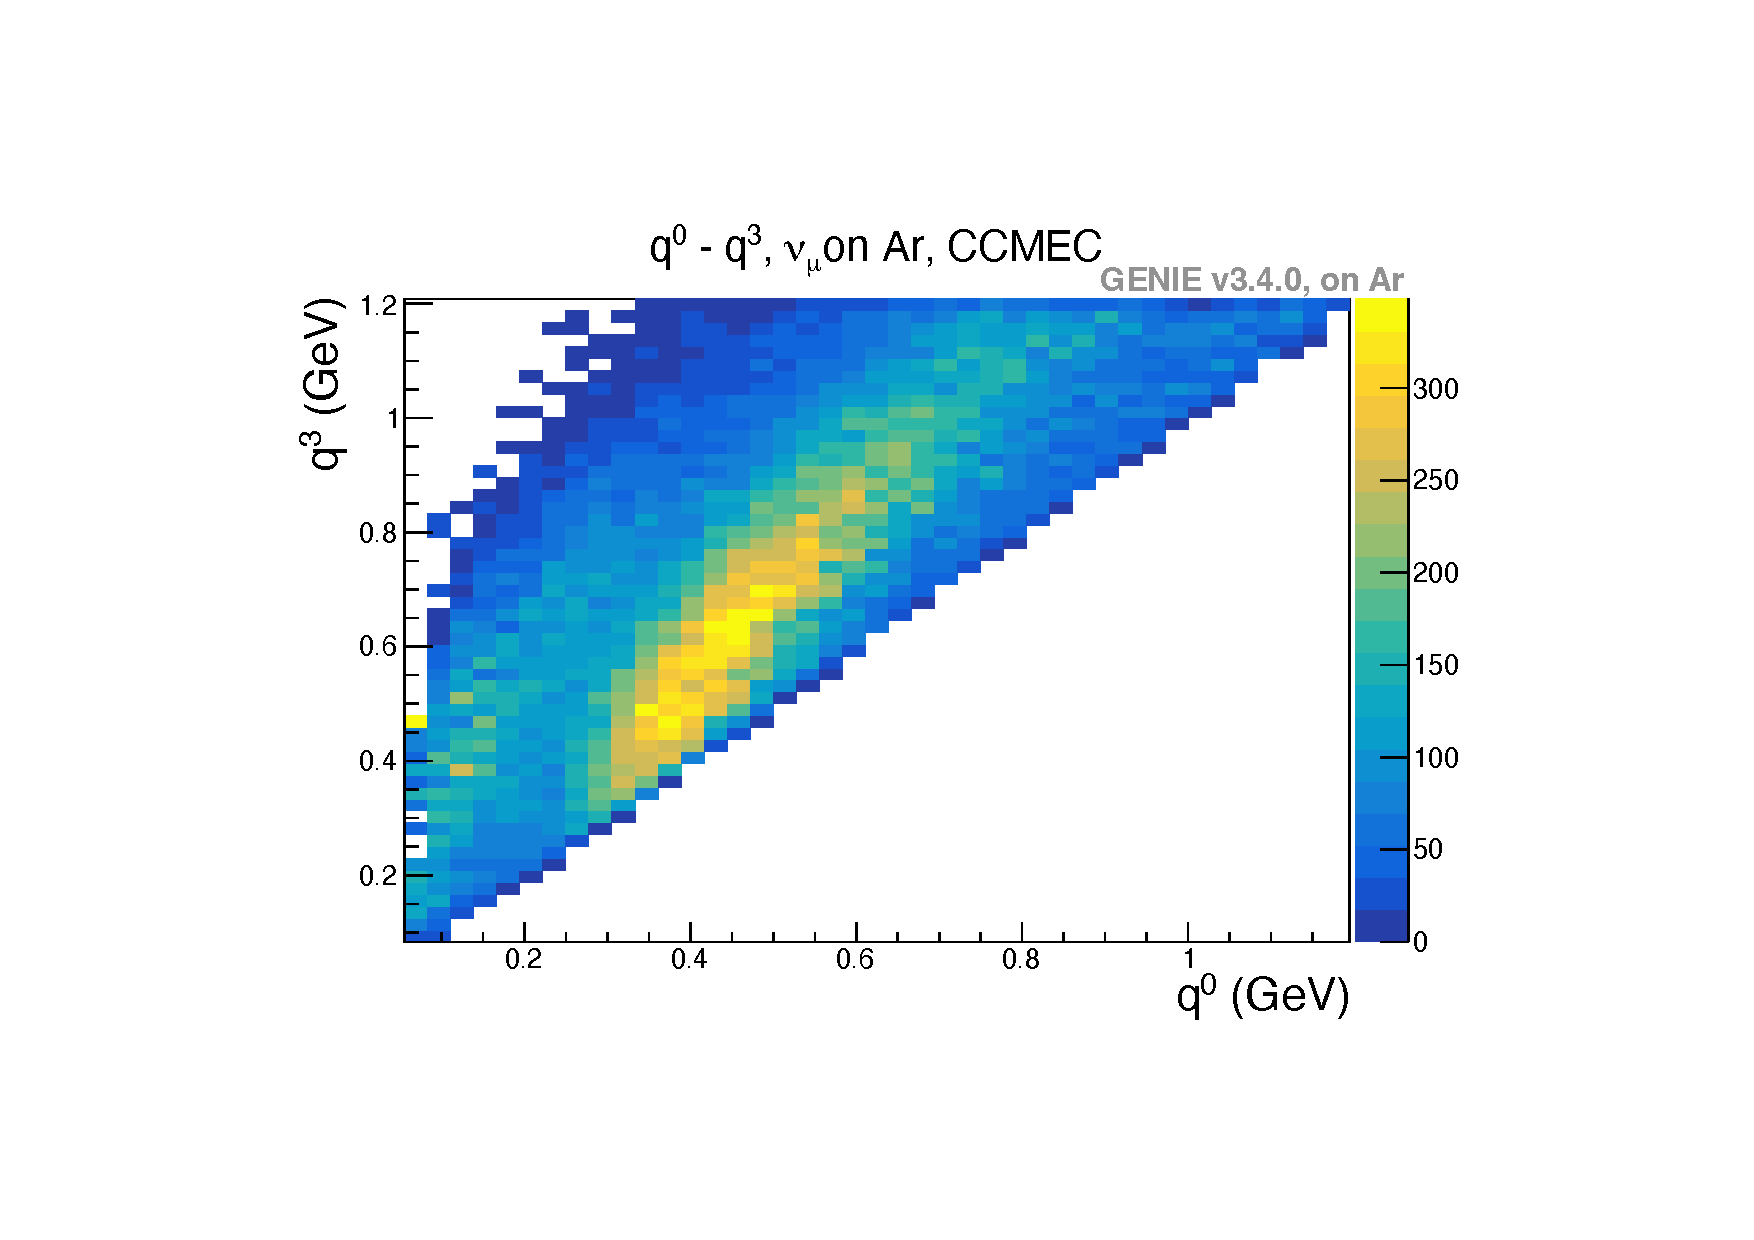
\includegraphics[width=\textwidth]{figures/XSecShape_CCMEC/2DComp_q0-q3_SuSAv2->Valencia_edited.pdf}
        \vspace{-2.mm}
%	\caption{}
	\label{xsecshapeccmec_b}
    \end{subfigure}
	\begin{subfigure}[b]{.32\textwidth}
        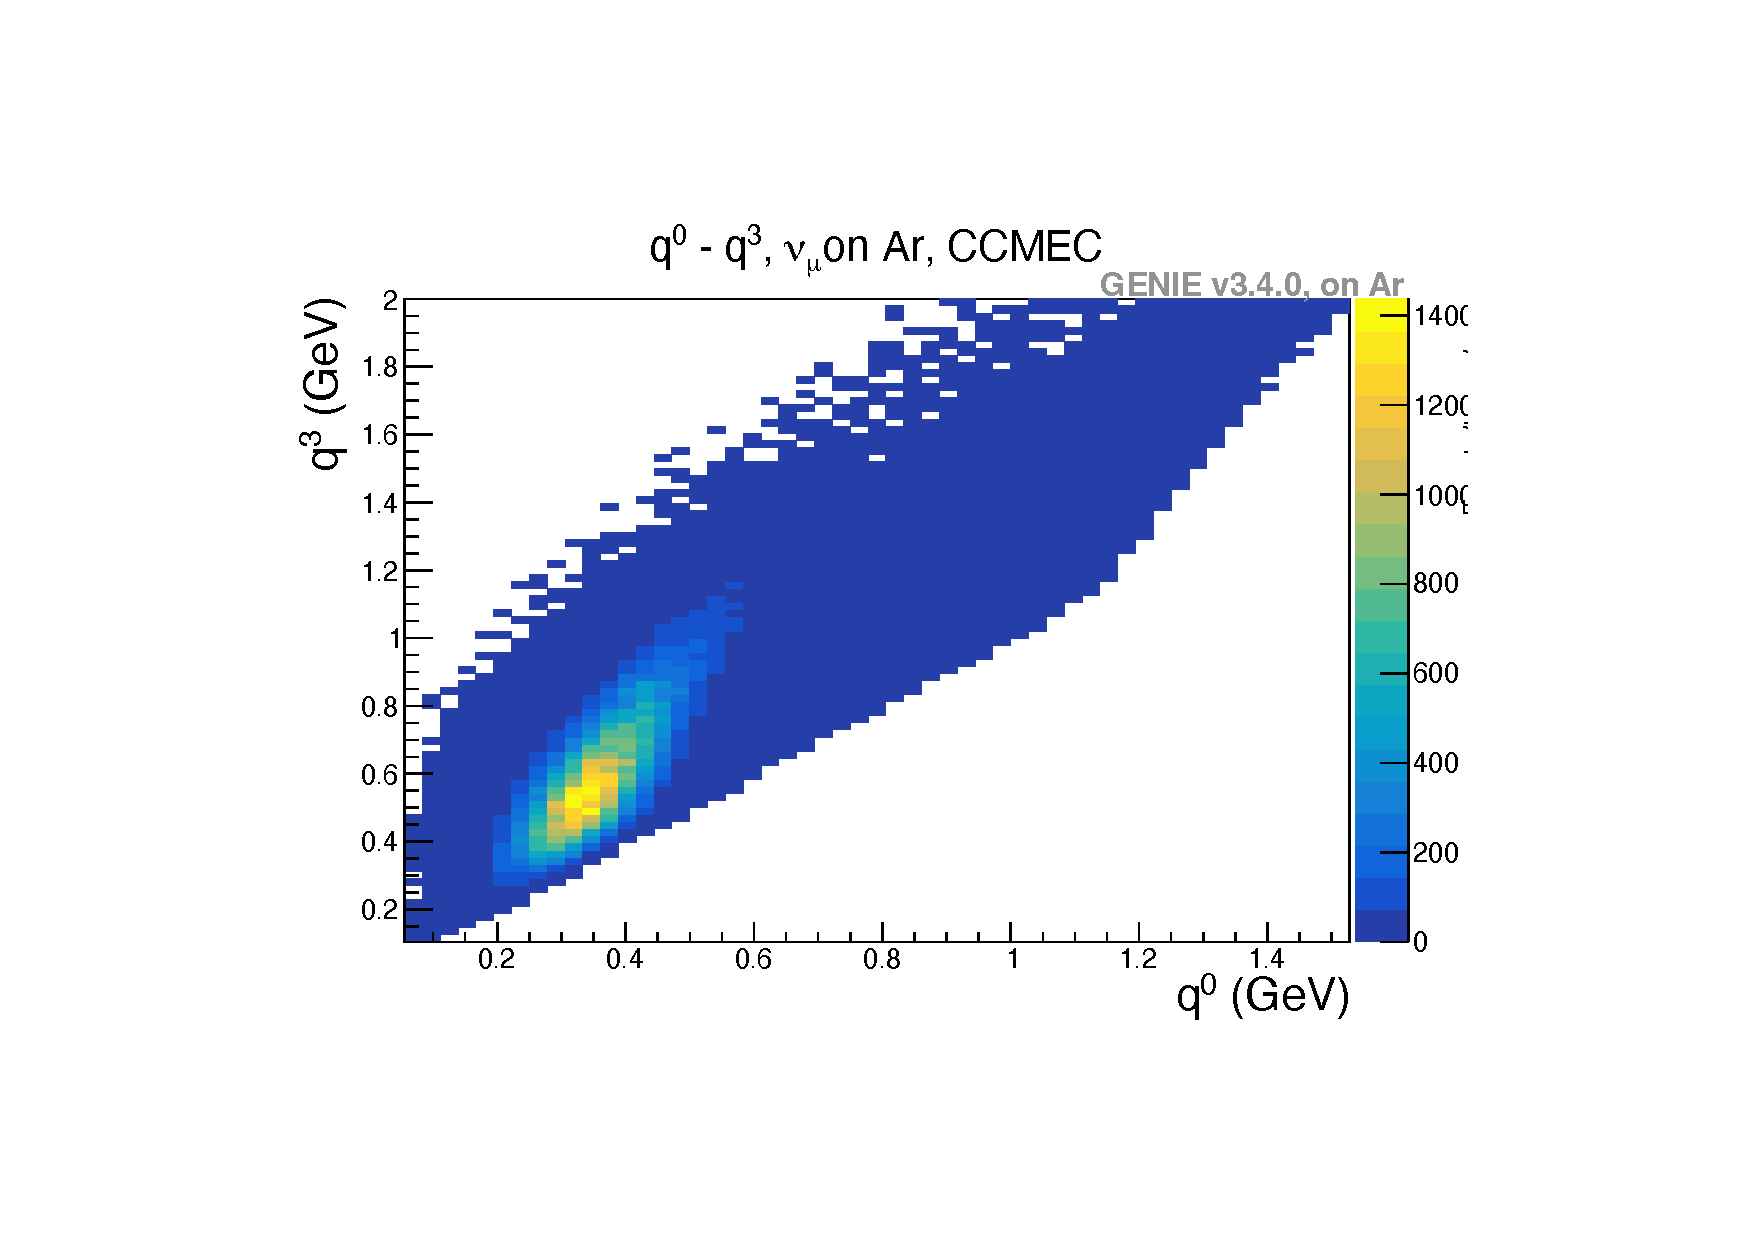
\includegraphics[width=\textwidth]{figures/XSecShape_CCMEC/2DComp_q0-q3_SuSAv2->Empirical_edited.pdf}
        \vspace{-2.mm}
%	\caption{}
	\label{xsecshapeccmec_c}
    \end{subfigure}
    \vspace{-6mm}
	\caption[]{XSecShape\_CCMEC parameter dials. The $q^0-q^3$ distributions are area-normalised.}
	\label{xsecshapeccmec}
\end{figure}
%
\fi
The Valencia-to-Martini et al. reweighting shown in \Cref{fig:xsecshape_valenciaTomartini} modifies the initially well-separated two-peak structure into a distribution resembling the overlapping peaks predicted by the Martini et al. model. Furthermore, the energy-transfer limitation $\omega<\SI{0.995}{\GeV}$ suppresses events above this threshold (middle panel) and ultimately removes them entirely in the fully reweighted distribution.
%
    \begin{figure}[H]
	\centering
	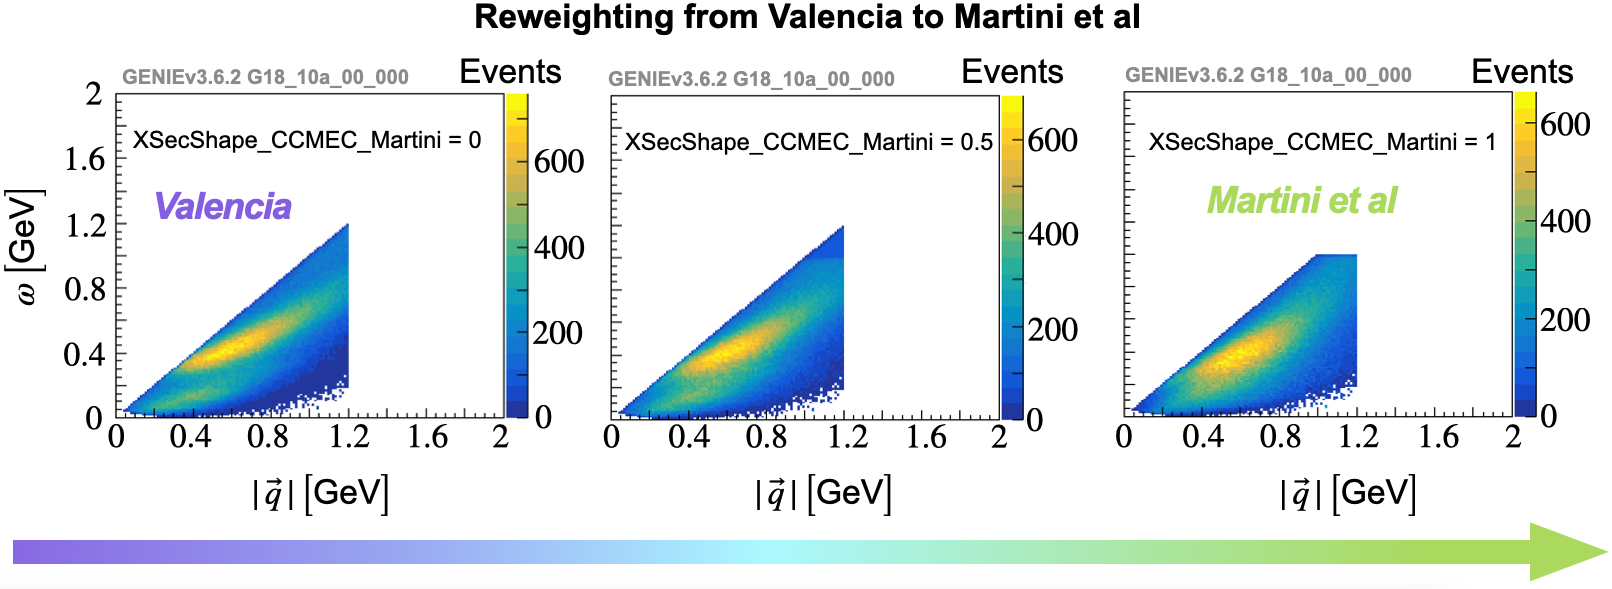
\includegraphics[width=\textwidth]{figures/XSecShape_CCMEC/xsecshape_valenciaTomartini.png}
	\caption[\texttt{XSecShape\_CCMEC\_Martini} Parameter: Reweighting from the Valencia to the Martini et al. Model]{\texttt{XSecShape\_CCMEC\_Martini} Parameter: Reweighting from the Valencia to the Martini et al. model.}
	\label{fig:xsecshape_valenciaTomartini}
    \end{figure}
%
Similar behaviour is observed for reweighting from the SuSAv$2$ model (Figs. (\ref{fig:xsecshape_susav2Tovalencia})-(\ref{fig:xsecshape_susav2Tomartini})) and from the Martini et al. model (Figs. (\ref{fig:xsecshape_martiniTovalencia})-(\ref{fig:xsecshape_martiniTosusav2})).
%
    \begin{figure}[H]
	\centering
	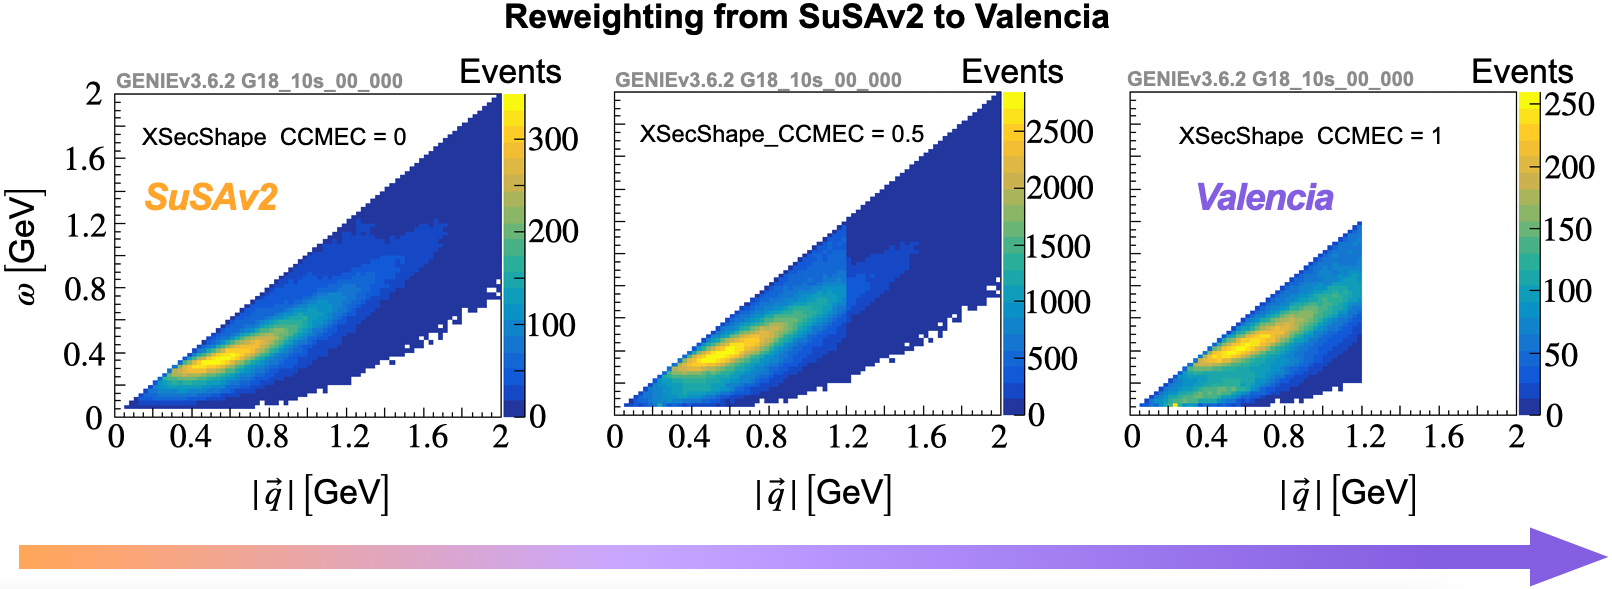
\includegraphics[width=\textwidth]{figures/XSecShape_CCMEC/xsecshape_susav2Tovalencia.png}
	\caption[\texttt{XSecShape\_CCMEC} Parameter: Reweighting from the SuSAv$2$ to the Valecencia Model]{\texttt{XSecShape\_CCMEC} Parameter: Reweighting from the SuSAv$2$ to the Valencia model.}
	\label{fig:xsecshape_susav2Tovalencia}
    \end{figure}
%
%
    \begin{figure}[H]
	\centering
	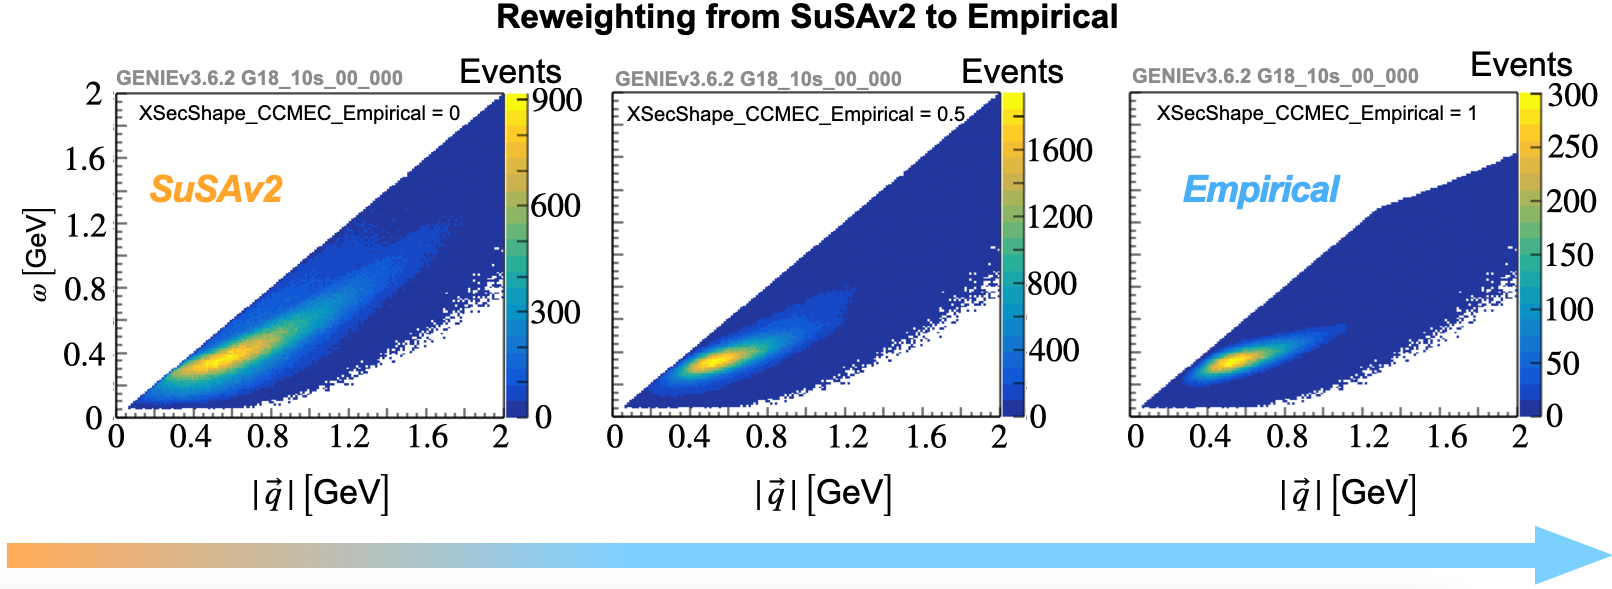
\includegraphics[width=\textwidth]{figures/XSecShape_CCMEC/xsecshape_susav2Toempirical.png}
	\caption[\texttt{XSecShape\_CCMEC\_Empirical} Parameter: Reweighting from the SuSAv2 to the Empirical Model]{\texttt{XSecShape\_CCMEC\_Empirical} Parameter: Reweighting from the SuSAv2 to the Empirical model.}
	\label{fig:xsecshape_susav2Toempirical}
    \end{figure}
%
%
    \begin{figure}[H]
	\centering
	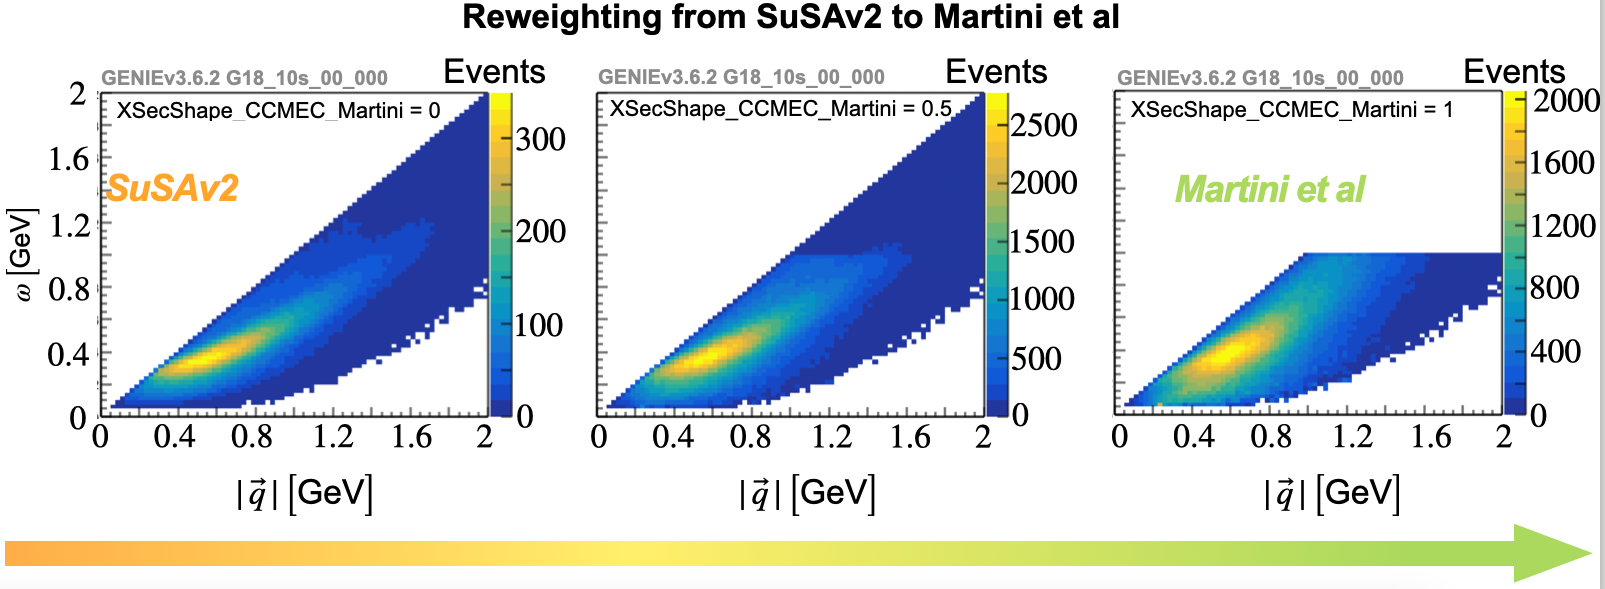
\includegraphics[width=\textwidth]{figures/XSecShape_CCMEC/xsecshape_susav2Tomartini.png}
	\caption[\texttt{XSecShape\_CCMEC\_Martini} Parameter: Reweighting from the SuSAv2 to the Martini et al. Model]{\texttt{XSecShape\_CCMEC\_Martini} Parameter: Reweighting from the SuSAv2 to the Martini et al. model.}
	\label{fig:xsecshape_susav2Tomartini}
    \end{figure}
%
%
    \begin{figure}[H]
	\centering
	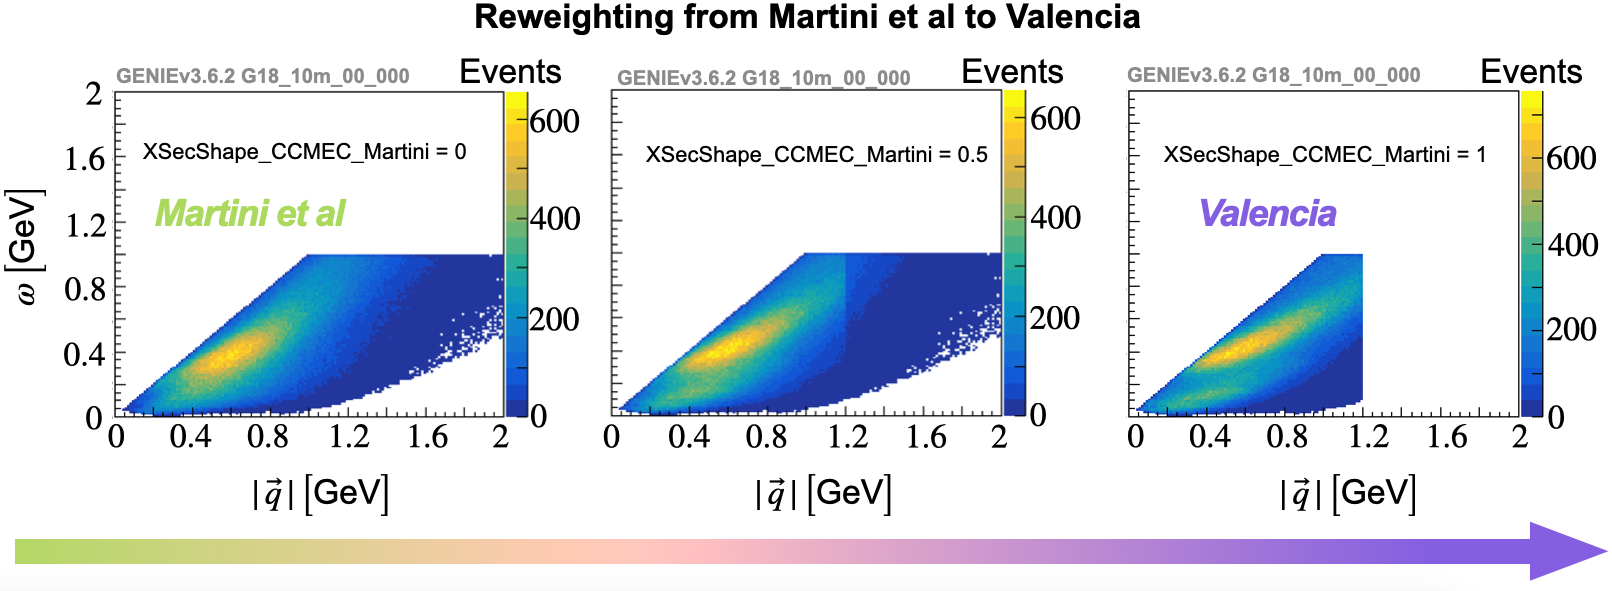
\includegraphics[width=\textwidth]{figures/XSecShape_CCMEC/xsecshape_martiniTovalencia.png}
	\caption[\texttt{XSecShape\_CCMEC\_Martini} Parameter: Reweighting from the Martini et al. to the Valencia Model]{\texttt{XSecShape\_CCMEC\_Martini} Parameter: Reweighting from the Martini et al. to the Valencia model.}
	\label{fig:xsecshape_martiniTovalencia}
    \end{figure}
%
%
    \begin{figure}[H]
	\centering
	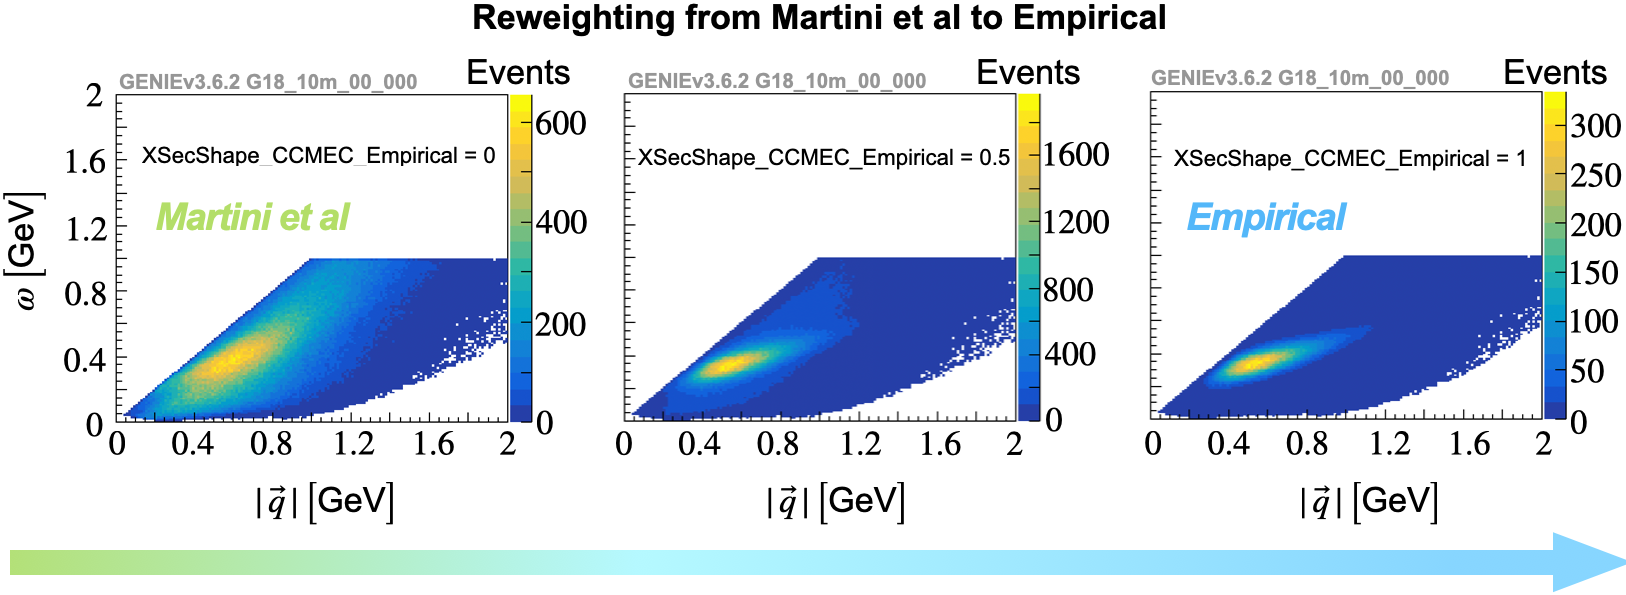
\includegraphics[width=\textwidth]{figures/XSecShape_CCMEC/xsecshape_martiniToempirical.png}
	\caption[\texttt{XSecShape\_CCMEC\_Empirical} Parameter: Reweighting from the Martini et al. to the Empirical Model]{\texttt{XSecShape\_CCMEC\_Empirical} Parameter: Reweighting from the Martini et al. to the Empirical model.}
	\label{fig:xsecshape_martiniToempirical}
    \end{figure}
%
%
    \begin{figure}[H]
	\centering
	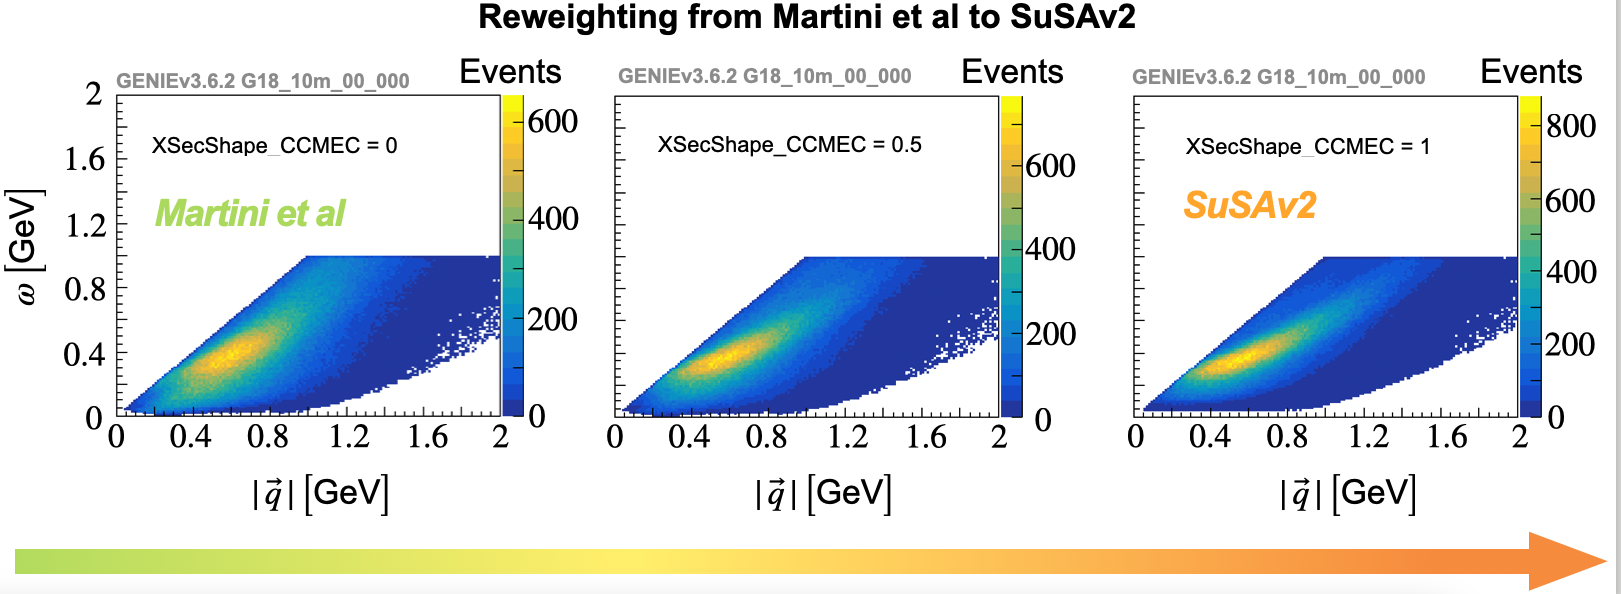
\includegraphics[width=\textwidth]{figures/XSecShape_CCMEC/xsecshape_martiniTosusav2.png}
	\caption[\texttt{XSecShape\_CCMEC} Parameter: Reweighting from the Martini et al. to the SuSAv2 Model]{\texttt{XSecShape\_CCMEC} Parameter: Reweighting from the Martini et al. to the SuSAv2 model.}
	\label{fig:xsecshape_martiniTosusav2}
    \end{figure}
%
The results presented in this section demonstrate how the cross-section shape parameters continuously morph the kinematic response between different theoretical model predictions.
There is good agreement between the fully reweighted distributions and the nominal predictions. \Cref{fig:xsecshape_overview} summarises all possible combinations of reweighting in the current \acrshort{genie} Reweight implementation.
%
\begin{landscape}
    \begin{figure}[p]
	\centering
	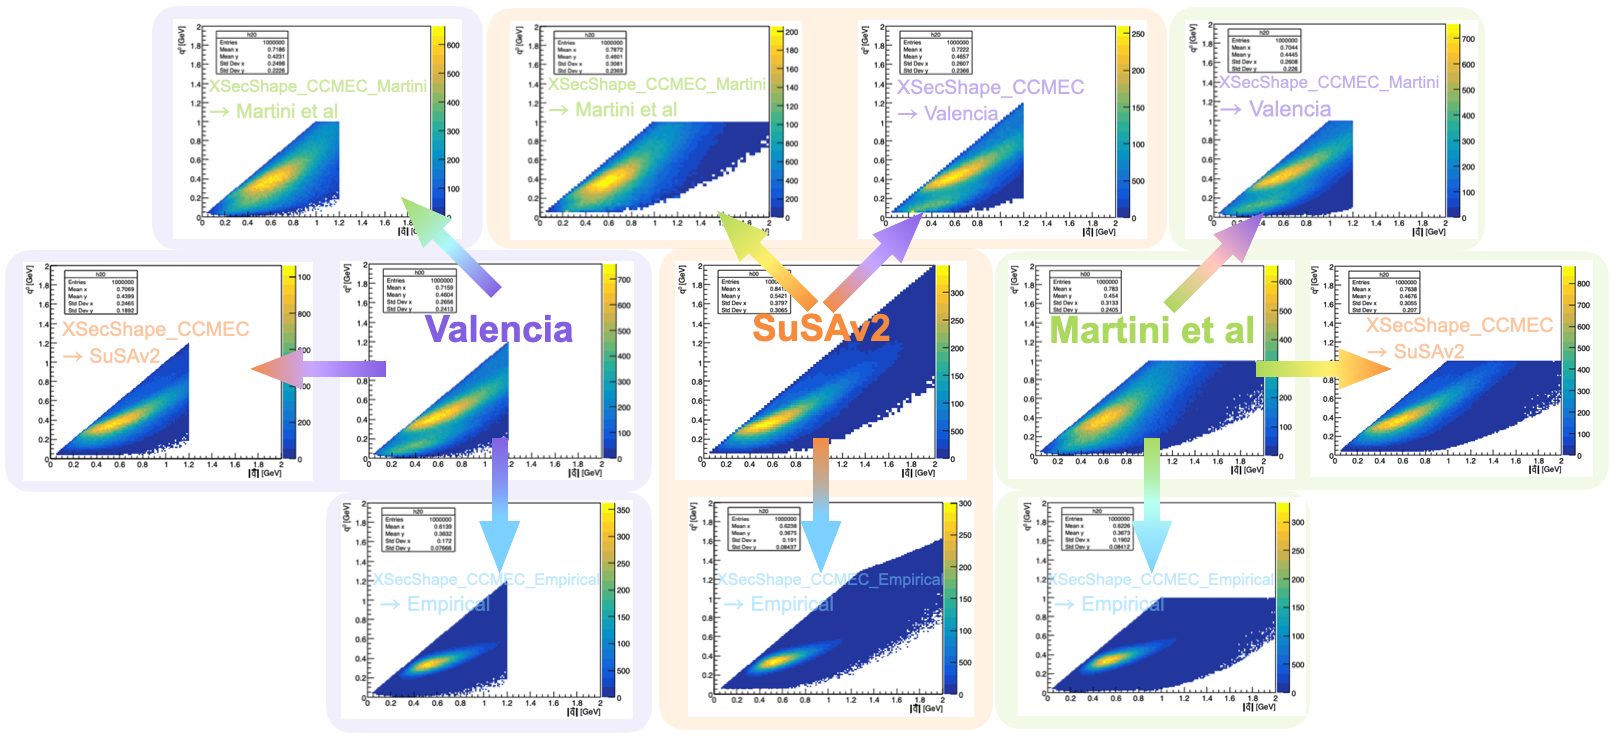
\includegraphics[height=0.73\textheight]{figures/XSecShape_CCMEC/xsecshape_overview.png}
    \caption[Cross-Section Shape Parameter Overview]{Cross-section shape parameter overview in the $\omega- |\vec{q}|$ phase space. The three central panels show the nominal predictions for the Valencia (purple, left), SuSAv$2$ (orange, middle) and Martini et al. (green, right) models. The surrounding panels illustrate the effect of the shape reweighting parameters, with arrows and colours indicating the direction of interpolation from the central nominal default model to the fully reweighted, alternative target model. The \texttt{XSecShape\_CCMEC} parameter interpolates between the Valencia and SuSAv2 models and maps Martini et al. towards SuSAv$2$. The \texttt{XSecShape\_CCMEC\_Empirical} parameter reweights all models towards the Empirical prediction. The \texttt{XSecShape\_CCMEC\_Martini} interpolates to the Martini et al. model and Martini et al. towards Valencia. The correspondence between default and target models for each parameter is summarised in \Cref{tab:xsecshape_summary}. Intermediate reweighting stages are shown in Figs. (\ref{fig:xsecshape_valenciaTosusav2}–(\ref{fig:xsecshape_martiniTosusav2}), illustrating the continuous deformation of the kinematic distributions as the interpolation parameter is varied.}
	\label{fig:xsecshape_overview}
    \end{figure}
%
\end{landscape}
%

\subsection{Energy Dependence of Cross Section} \label{sec:edep_ccmec}
The energy dependence parameter changes the neutrino-energy dependence of the \acrshort{2p2h} cross section. Different models have different predictions on the energy dependence of the cross section as shown in the left plot in \cref{fig:edep_normalisation}).
%
    \begin{figure}[H]
	\centering
	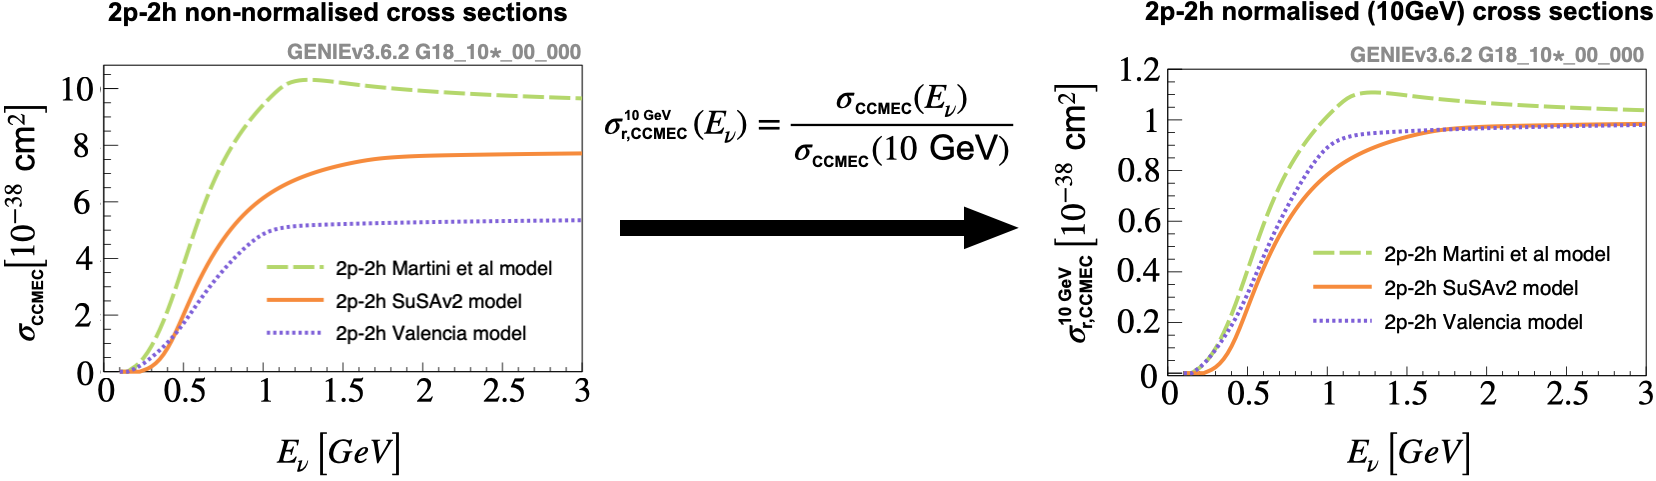
\includegraphics[width=\textwidth]{figures/Energy_Dependence_CCMEC/edep_normalisation.png}
	\caption[Parameter to Adjust the Energy Dependence of the Cross Section]{Parameter to adjust the energy dependence of the cross section. Left: The different \acrshort{cc} \acrshort{2p2h} model predictions by the Valencia, SuSAv2 and Martini et al. models as a function of the neutrino energy $E_\nu$. Right: The renormalised cross-section predictions for an anchoring point of $\SI{10}{\GeV}$.}
	\label{fig:edep_normalisation}
    \end{figure}
%
To isolate shape differences in the energy dependence, the cross sections are renormalised by introducing an anchoring point at a fixed neutrino energy\footnote{Similar approaches have been developed in \acrshort{t2k} \cite{t2k-niwg} and No$\nu$a \cite{NOvA:2020rbg}.}. This ensures that all models coincide at that energy while preserving their relative shape differences. In this work, the anchoring point is chosen at a relatively high energy, $\SI{10}{\GeV}$, such that deviations at lower energies are emphasised.
The renormalised cross sections
%
\begin{align} \label{eq:edep_xsec_normalisation}
    \sigma^{10\text{ GeV}}_\text{r,CCMEC}(E_\nu) = \frac{\sigma_\text{CCMEC}(E_\nu)}{\sigma_\text{CCMEC}(\SI{10}{\GeV})}
\end{align}
%
are shown in the right plot in \cref{fig:edep_normalisation}. As the differences between the renormalised cross-section model predictions are largest for neutrino energies below $\SI{1.5}{\GeV}$, the energy-dependence reweighting primarily affects the low-energy region. This behaviour is a direct consequence of choosing the anchoring point at relatively high energy.
The ratio
%
\begin{align} \label{eq:edep_ratio}
    r(E_\nu) = \frac{\sigma^\text{alt}_\text{r,CCMEC}(E_\nu)}{\sigma^\text{def}_\text{r,CCMEC}(E_\nu)} \ \text{,}
\end{align}
%
between the renormalised cross section of the alternative and the default model is a function which envelopes the renormalised cross section variations as shown in \Cref{fig:edep_normalisation_uncBand}.
%
    \begin{figure}[H]
	\centering
	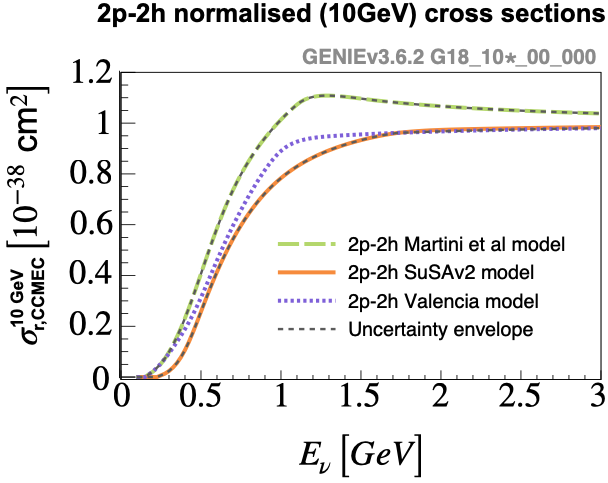
\includegraphics[width=0.8\textwidth]{figures/Energy_Dependence_CCMEC/edep_normalisation_uncBand.png}
	\caption[Uncertainty Band for the \texttt{EnergyDependence\_CCMEC} Reweighting]{Uncertainty Band for the \texttt{EnergyDependence\_CCMEC} Reweighting. The \acrshort{cc} \acrshort{2p2h} renormalised cross section predictions by the Valencia (dotted purple), SuSAv$2$ (solid orange) and Martini et al. (dashed green) models overlaid with the uncertainty envelope (dashed gray) obtained by the ratio function in \Cref{eq:edep_ratio}.}
	\label{fig:edep_normalisation_uncBand}
    \end{figure}
%
The ratio in \Cref{eq:edep_ratio} functions as a energy-dependent \acrshort{2p2h} normalisation uncertainty bands used to define the weight associated with the energy-dependence parameter $\verb!EnergyDependence_CCMEC!$:
%
\begin{align} \label{eq:edep_xsec_parametrisation}
    \sigma_\nu(E_\nu) = \sigma_\nu^{nom}(E_\nu) \cdot \underbrace{ \left( 1+x_E\left(r(E_\nu)-1\right) \right)}_{w^\text{EnergyDependence\_CCMEC}} \ \text{,}
\end{align}
%
The ratio in \Cref{eq:edep_ratio} defines the relative deviation between
the alternative and default model predictions. In combination with setting the tweak dial $x_E$, ratios $r \equiv r^\text{up}_\text{UncBand} > 1$ enhance the cross-section at a given energy to the maximum cross-section model prediction. Ratios $r \equiv r^\text{down}_\text{UncBand} < 1$ lower the cross-section at a given energy to the minimum cross-section model prediction. Depending on the sign of the dial $x_E$, the following ratios $r$ are used for the weight computation in \cref{eq:edep_xsec_parametrisation}:
%
\begin{align}       \label{eq:edep_dial_cases}
    r =
    \begin{cases} 
        r^\text{up}_\text{UncBand} & \text{if } \ x_E > 0 \\
        r = 1 & \text{if } \ x_E = 0 \\
        r = r^\text{down}_\text{UncBand} & \text{if } \ x_E < 0
    \end{cases}
\end{align}
%
The effect of the \verb!EnergyDependence_CCMEC! parameter depends on the
position of the nominal model within the uncertainty band defined by the
ratio function in \Cref{eq:edep_ratio}. Variations of the tweak dial $x_E$
interpolate between these predictions, leading to the largest deviations
at low neutrino energies.

The effect of varying the \verb!EnergyDependence_CCMEC! tweak dial for the
nominal SuSAv2 model is shown in \Cref{fig:edep_susav2}. Over most of the
energy range, the SuSAv2 model predicts lower cross sections than the
Valencia and Martini et al.\ models. Consequently, negative values of the
tweak dial $x_E$ lead to only minor changes in the neutrino-energy
distribution, as the SuSAv2 prediction already lies close to the lower
edge of the uncertainty band. 

In contrast, positive values of $x_E$ enhance the neutrino-energy
distribution, reflecting the higher cross-section predictions of the
Martini et al.\ model. Deviations are most pronounced at low energies,
while increasingly smaller differences are observed above $E_\nu \approx \SI{4}{\GeV}$.
%
    \begin{figure}[htb]
	\centering
	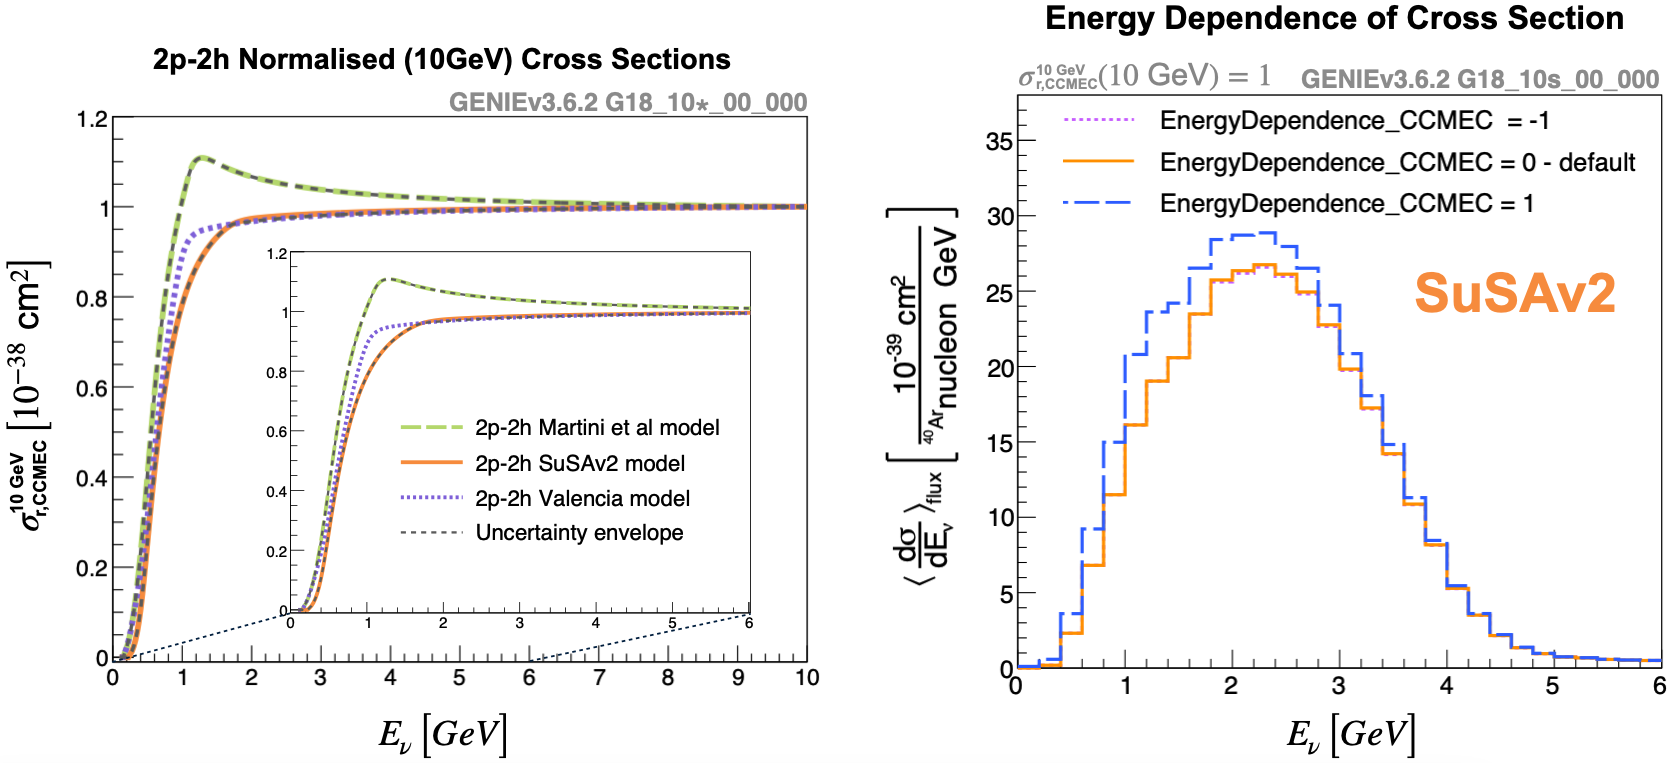
\includegraphics[width=\textwidth]{figures/Energy_Dependence_CCMEC/edep_susav2.png}
	\caption[Reweighting of the SuSAv2 Model to Modify the Energy Dependence of the Cross Section]{Reweighting of the SuSAv2 model to modify the energy dependence of the cross section using the \texttt{EnergyDependence\_CCMEC} parameter. The renormalised cross-section with uncertainty band (dotted gray) is shown on the left. The neutrino-energy distribution with tweak dial variations are shown on the right.}
	\label{fig:edep_susav2}
    \end{figure}
%
For the Valencia model in the left plot in \Cref{fig:edep_valencia_martini}, which lies between the
other predictions below $E_\nu \approx \SI{1.8}{\GeV}$, both positive and negative variations of $x_E$ lead to
visible changes, interpolating towards the Martini et al.\ and SuSAv2
models, respectively.

For the Martini et al.\ model in the right plot in \Cref{fig:edep_martini}, which predicts
the highest cross sections, positive values of $x_E$ have no effect as the Martini model defines the upper uncertainty band. However, negative values of $x_E$ reduce the distribution towards the lower Valencia
and SuSAv2 predictions.
%
\begin{figure}[H]
\centering

\begin{subfigure}[htb]{0.485\textwidth}
    \centering
    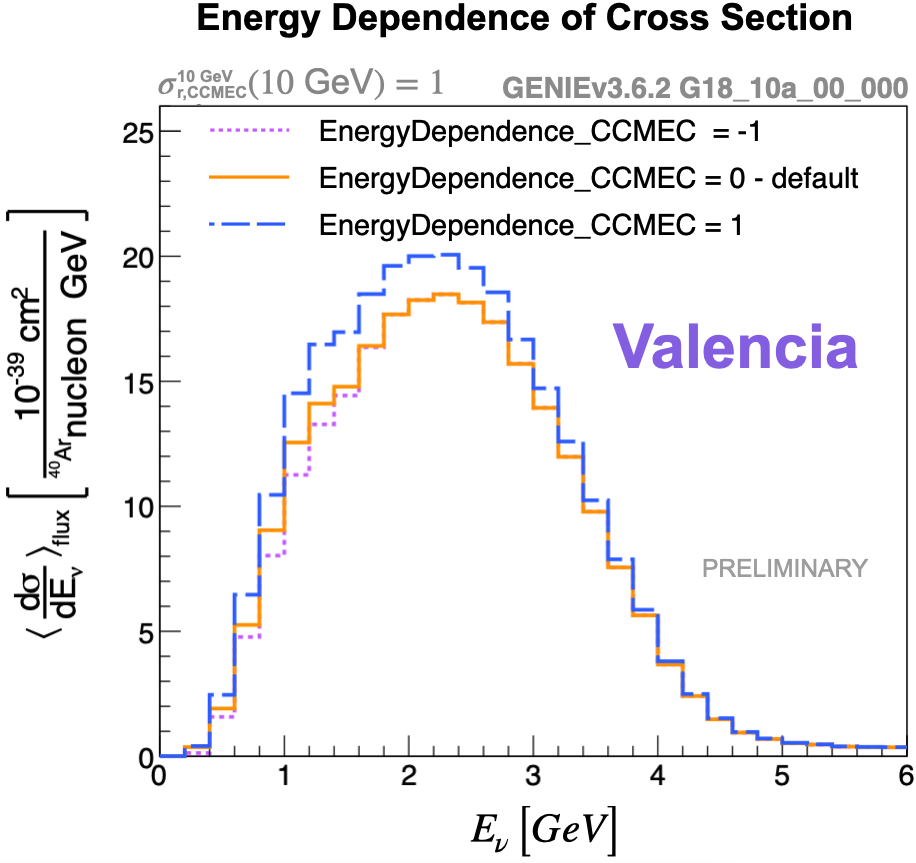
\includegraphics[width=\linewidth]{figures/Energy_Dependence_CCMEC/edep_valencia.png}
    %\caption{Valencia model.}
    %\label{fig:edep_valencia_left}
\end{subfigure}
\hfill
\begin{subfigure}[htb]{0.495\textwidth}
    \centering
    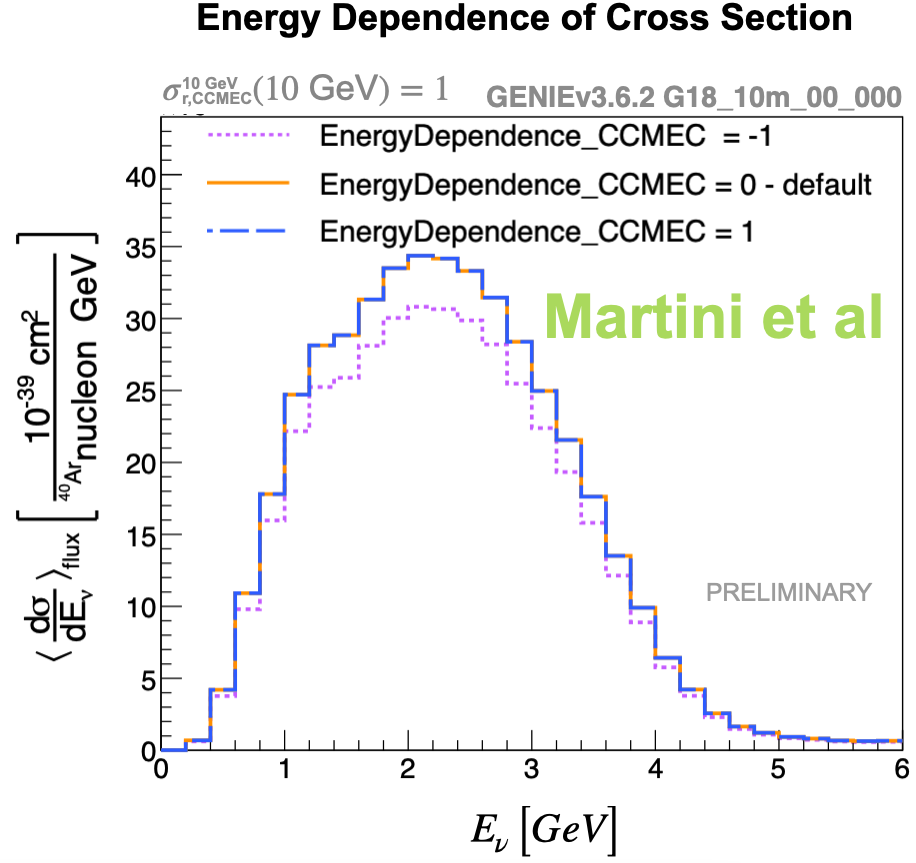
\includegraphics[width=\linewidth]{figures/Energy_Dependence_CCMEC/edep_martini.png}
    %\caption{Reweighted Martini model.}
    %\label{fig:edep_valencia_right}
\end{subfigure}
%
\caption[Reweighting of the Valencia and Martini et al. Models to Modify the Energy Dependence of the Cross Section]{Reweighting of the Valencia and Martini et al. models to modify the energy dependence of the cross section using the \texttt{EnergyDependence\_CCMEC} parameter.}
\label{fig:edep_valencia_martini}
\end{figure}
%
\iffalse
%
    \begin{figure}[H]
	\centering
	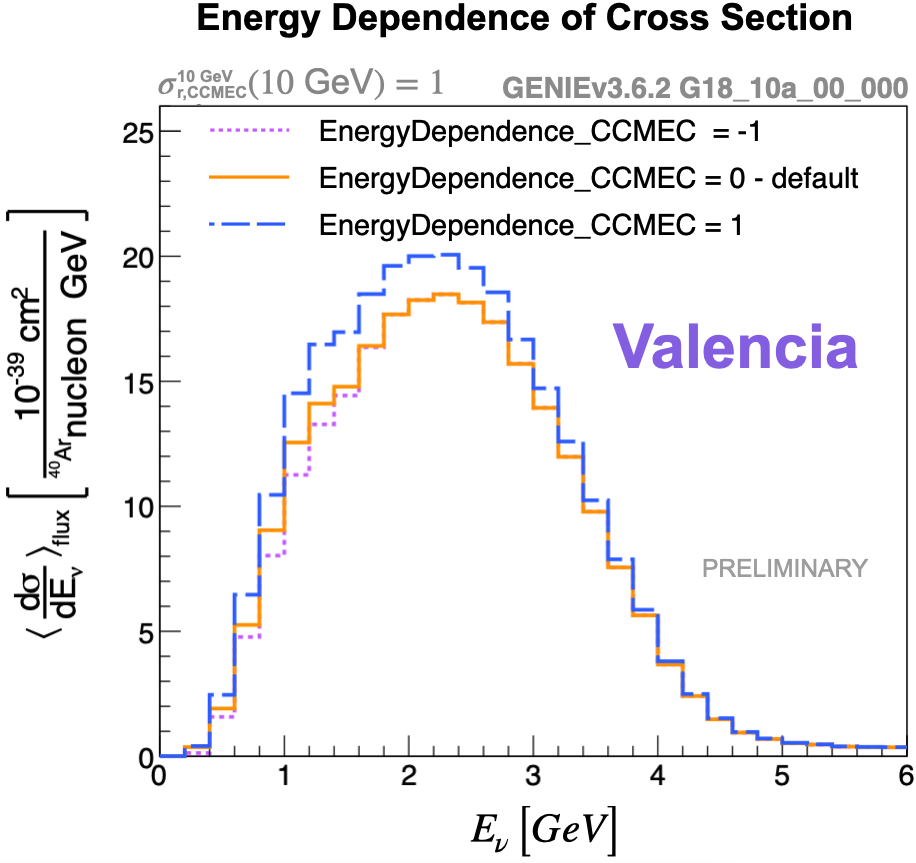
\includegraphics[width=\textwidth]{figures/Energy_Dependence_CCMEC/edep_valencia.png}
	\caption[Reweighting of the Valencia Model to Modify the Energy Dependence of the Cross Section]{Reweighting of the Valencia model to modify the energy dependence of the cross section using the \texttt{EnergyDependence\_CCMEC} parameter.}
	\label{fig:edep_valencia}
    \end{figure}
%
%
    \begin{figure}[H]
	\centering
	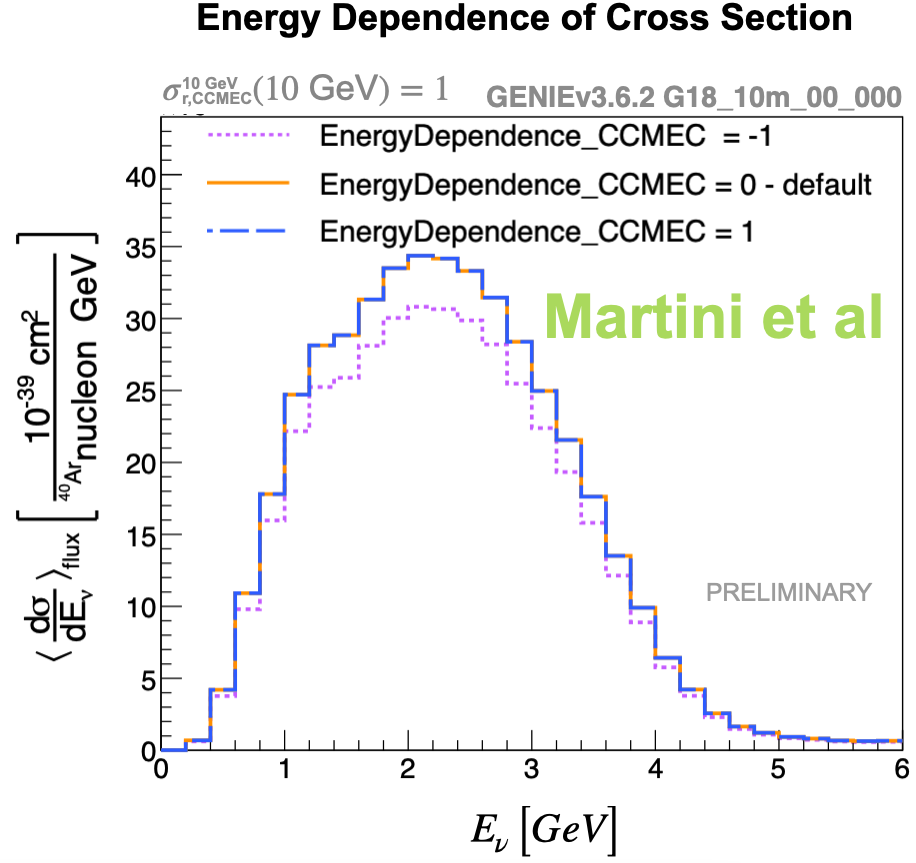
\includegraphics[width=\textwidth]{figures/Energy_Dependence_CCMEC/edep_martini.png}
	\caption[Reweighting of the Martini et al. Model to Modify the Energy Dependence of the Cross Section]{Reweighting of the Martini et al. model to modify the energy dependence of the cross section using the \texttt{EnergyDependence\_CCMEC} parameter.}
	\label{fig:edep_martini}
    \end{figure}
%
\fi

\subsection{MC-Data Comparison}
\textcolor{red}{May leave out this section.}

\section{Conclusion and Outlook} \label{conclusion_syst}
A summary of the \acrshort{cc} \acrshort{2p2h} uncertainty parameters that are implemented in GENIE Reweight are shown in \cref{tab:xsecshape_summary}.
In this thesis, new systematic parameters associated with uncertainties in the modeling of \acrfull{cc} \acrshort{2p2h} neutrino-nucleus interactions were developed and implemented in the GENIE Reweight framework. Their impact on selected observables was studied and
validated, demonstrating their suitability for uncertainty propagation
in oscillation analyses.

Several avenues for further development of systematic parameters remain. 
For example, there is currently no implementation of the nucleon angular distribution parameter $\verb!DecayAngMEC!$ that considers the dependence on hadron kinematics in the momentum transfer to the struck nucleon pair. A semi-inclusive approach can be found in \cite{PhysRevC.109.015502}.
Another possible extension is the reweighting between imbalanced and back-to-back nucleon configurations \cite{Bathe-Peters:2022kkj}.
In addition, further parameters could be introduced to account for uncertainties in the removal energy carried away by the struck nucleon pair. 

Furthermore, the reweighting framework should be extended to anti-neutrino scattering, especially for parameters affecting the cross-section shape interpolation and the $\verb!EnergyDependence_CCMEC!$ parameter considering the energy dependence of the cross section. A more sophisticated treatment of the energy dependence could be achieved by modifying the structure functions $W_i$ ($i=1,\dots,5$) in the hadronic tensor \cite{osti_1996929}. This could potentially be realised by introducing independent tweak dials controlling the strength of the individual structure functions $W_i$ in \Cref{eq:vary_structure_func}.
%
\begin{align} \label{eq:vary_structure_func}
    \frac{\overline{L}_{\mu\nu} \overline{W}^{\mu\nu}}{E_\nu^2} 
    &=
    \frac{1}{E_\nu^2}\Big[
    W_1 (Q^2 + m_l^2)
    - \frac{W_2}{2}(m_l^2 + Q^2)
    \mp \frac{q_0 W_3}{2M} (m_l^2 + Q^2) \notag \\
    &\quad
    + \frac{W_4}{M^2} \frac{Q^2 m_l^2 + m_l^4}{2}
    \Big]
    + \frac{1}{E_\nu} \Big[
    -2q_0 W_2 \pm \frac{W_3 Q^2}{M}
    - \frac{W_5 m_l^2}{M}
    \Big]
    + W_2 \,.
    \end{align}
%

Improving the consistency between theoretical calculations and their
implementation in Monte Carlo generators remains essential
\cite{Sobczyk:2020dkn}. 
%
    \begin{figure}[htb]
	\centering
	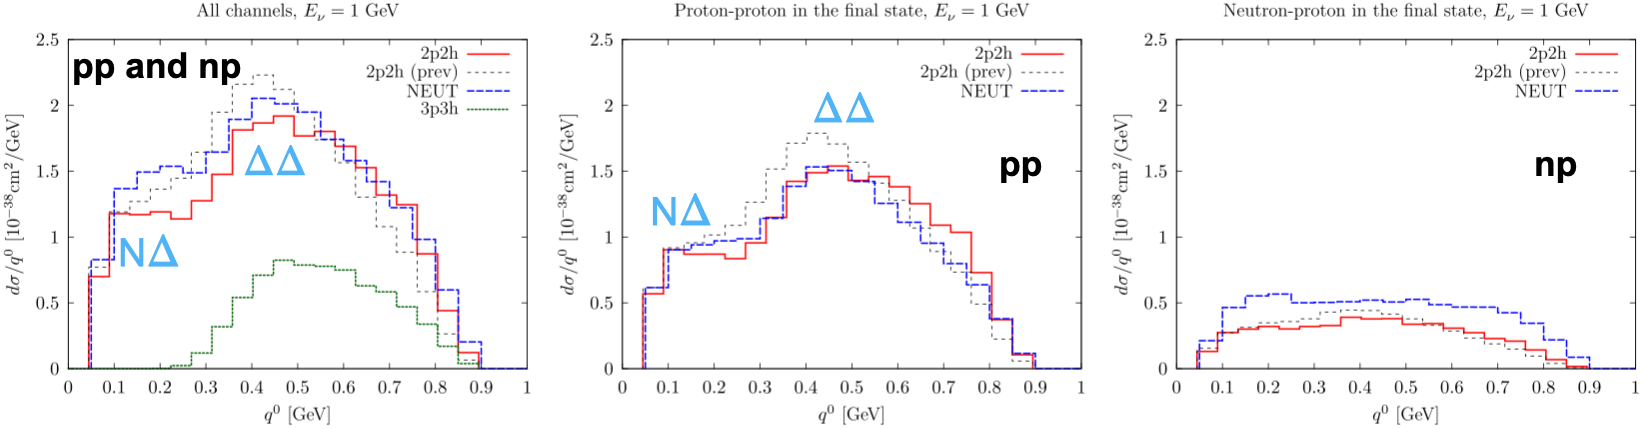
\includegraphics[width=\textwidth]{figures/x-secs/generator_theory_tension.png}
	\caption[Tension between Theory and Generator Predictions]{Tension between Theory and Generator Predictions. The differential cross sections $\frac{\mathrm{d}\sigma}{\mathrm{d}\omega}$ with respect to the leptonic momentum transfer $\omega \equiv q^0$ on $^{12}$C for a neutrino energy $E_\nu = \SI{1}{\GeV}$. The left distribution is summed over isospin. Its split into two protons (pp, middle) and one proton and one neutron (np, right) in the final state are shown for better comparison between theory and generator predictions. Two previous implementations of the \acrshort{2p2h} Valencia model are shown (solid red and dashed gray) alongside the 3p-3h prediction (solid green) and the generator (NEUT, dashed blue) result. Figure adapted from \cite{Sobczyk:2020dkn}.}
	\label{fig:generator_theory_tension}
    \end{figure}
%
As illustrated in \Cref{fig:generator_theory_tension}, significant discrepancies persist between generator predictions (e.g. NEUT) and theoretical results for \acrshort{2p2h} processes. In the comparison with the \acrshort{2p2h} Valencia model as shown in \Cref{fig:generator_theory_tension}, NEUT predicts larger cross sections for np-pair final states, which may partially originate from the inclusion of $3$p-$3$h contributions in NEUT. Such differences between theoretical and simulation predictions highlight the need for improved agreement between theoretical predictions and implementations in MC event generators, in addition to comparisons with experimental data.

With future neutrino-oscillation experiments such as \acrshort{dune}
expected to collect an unprecedented amount of data, neutrino physics is transitioning from a statistics-limited regime to one dominated by systematic uncertainties.
In this context, the development of robust systematic uncertainty estimates for both oscillation and cross-section analyses in current and future experiments such as \acrshort{dune} is crucial for ensuring unbiased measurements. 
In addition, the use of higher-energy neutrino beams in the future increases the importance of understanding \acrshort{2p2h} interactions. In this regime, \acrshort{2p2h} processes become more relevant, highlighting the need for accurate modeling and reasonable uncertainty quantification of these contributions.

The availability of the parameters developed in this thesis within GENIE Reweight will enable
improved estimates of systematic uncertainties and enhanced sensitivity in current and future neutrino-oscillation and cross-section measurements. Ultimately, these developments contribute to the broader goal of achieving a consistent and reliable description of neutrino-nucleus interactions, which is essential for the precision era of neutrino-oscillation physics.
%
\newpage
\begin{landscape}
%
    \begin{figure}[H]
	\centering
	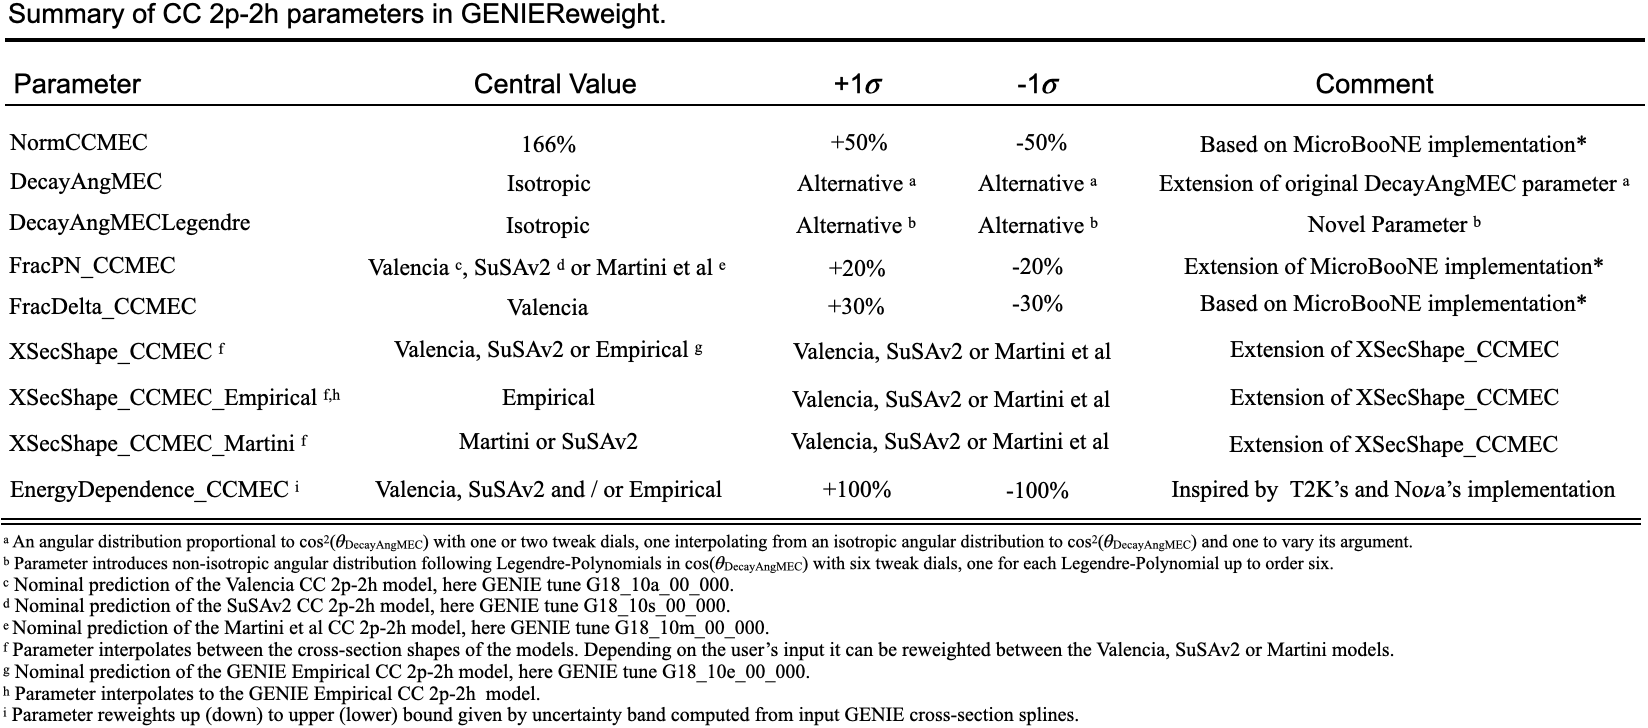
\includegraphics[width=\linewidth]{figures/systParams_sumTable.png}
	\caption[Summary of CC 2p-2h parameters in GENIEReweight]{Summary of CC 2p-2h parameters in GENIEReweight. Table adopted and extended from Table VIII in \cite{PhysRevD.105.072001}. For up-to-date information on the systematic parameter uncertainties, see \href{https://github.com/GENIE-MC/Reweight/blob/master/config/GSystUncertaintyTable.xml}{GENIE-MC/Generator/config/GSystUncertaintyTable.xml}.}
	\label{fig:systParams_sumTable.png}
    \end{figure}
%
\end{landscape}
\newpage